%% ====================================================================%%
%%	Sample Driver file for use with uwthesis.sty
%% 	To print this document in the Math Dept, 
%%	do the following:
%%  		latex main
%%		bibtex main
%%		latex main (you may have to do this twice at this point)
%%		dvipr main
%%	To run this sa mple, you will also need the following files
%%		abs.tex, ack.tex,
%%		chap1.tex, chap2.tex, appendix.tex	
%%		thesis.bib	
%% ====================================================================%%
%% 
\documentclass[11pt]{report}
\renewcommand{\familydefault}{\sfdefault}
\usepackage{helvet}
%% If you want to  process the graphics examples in Chap 3 uncomment this line

\usepackage{graphicx}
\usepackage[english]{babel}
\usepackage{textgreek}
\usepackage[backend=bibtex]{biblatex}
\addbibresource{mendeley.bib}
\usepackage[nottoc]{tocbibind} %Adds "References" to the table of contents
\usepackage[T1]{fontenc}

%\usepackage[square, numbers, sort&compress]{natbib}

\usepackage{StyleFiles/mythesis,StyleFiles/tgrind}
\usepackage{fancyhdr}
%% Use this if you only want to do Chap 1 things - basic stuff
%% NOTE: the uwthesis style file should go AFTER all the other packages
%% You may have conflicts if you call the amsthm.sty package after uwthesis.sty

\usepackage{amssymb,StyleFiles/uwthesis}

\graphicspath{
{./Chapters/Introduction/Figures/}
{./Chapters/HangingDroplet/Figures/}
{./Appendicies/HangingDroplet/Figures/}
}

\begin{document}

\title{Open Microfluidic Platforms for Tissue Culture}
\author{Theodorus E. de Groot}

%\inputpicturetrue  % By Jeff McGough. See uuguide and private thesis.sty
%\inputpicturefalse % To NOT produce pictures, uncomment this line


\degree{Doctor of Philosophy}
\dept{Biomedical Engineering}
\thesistype{dissertation}
%% Starts page numbering as i, ii, etc.
\beforepreface
\prefacesection{Abstract}
\input frontmatter/abs 
\prefacesection{Acknowledgements}



\input frontmatter/ack 
%\prefacesection{Papers}
% \input frontmatter/papers
\listoffigures
\listoftables

\afterpreface

%% Include the Chapters
\chapter{Chapter 1: Introduction}\label{Chap:Introduction}





\section{Preface}
Microfluidics are super useful, wow did you know that? I mean they really are the coolest! You can do some really cool stuff with microfluidics when you take off the lid and do open microfluidics. I'm super serious. It's really great. You can do stuff like make Legos or you could do some other stuff like culture cells and do tissue culture in ways that you never thought of before.

\section{Microfluidics for Tissue culture}
Let's talk about tissue culture platforms that used microfluidics because those are really important  n


\section{}
Wow Teddy, you're so smart\cite{Vogler2004a}.





\chapter{Surface-tension driven open microfluidic platform for hanging droplet culture}\footnote{This chapter has been modified from the published manuscript of the same title. The manuscript includes as authors Theodorus de Groot, Kelsey Veserat, Erwin Berthier, Ashleigh Theberge, and David Beebe}
\label{Chap:HangingDroplet}

The hanging droplet technique for three-dimensional tissue culture has been used for decades in biology labs, with the core technology remaining relatively unchanged. Recently microscale approaches have expanded the capabilities of the hanging droplet method, making it more user-friendly. We present a spontaneously driven, open hanging droplet culture platform to address many limitations of current platforms. Our platform makes use of two interconnected hanging droplet wells, a larger well where cells are cultured and a smaller well for user interface \textit{via} a pipette. The two-well system results in lower shear stress in the culture well during fluid exchange, enabling shear sensitive or non-adherent cells to be cultured in a droplet. The ability to perform fluid exchanges in-droplet enables long-term culture, treatment, and characterization without disruption of the culture. The open well format of the platform was utilized to perform time-dependent coculture, enabling culture configurations with bone tissue scaffolds and cells grown in suspension. The open nature of the system allowed the direct addition or removal of tissue over the course of an experiment, manipulations that would be impractical in other microfluidic or hanging droplet culture platforms. 


\section{Introduction}
Hanging droplet culture is perhaps the earliest 3D tissue culture system developed \cite{Harrison1910}. This method relies on the 3D self-assembly of a tissue spheroid from a cell suspension within a droplet suspended from the lid of a Petri dish. The earliest hanging droplet culture platform enabled the in vitro study of embryo development \cite{Harrison1910}, but the technique would later be used to study stem cell differentiation, tumorigenesis, bacteria \cite{Tittsler1936}, and even plant culture \cite{Muir1958}. In mammalian tissue culture, 3D techniques are capable of better replicating the in vivo environment, and observations made in 3D systems are often more physiologically relevant than in 2D cultures \cite{Abbott2003, Stegemann2003, Debnath2005, Folkman1973}. Despite the biological advances enabled by hanging droplet culture, the method has several limitations, including inconsistencies in droplet size and challenges accessing the culture for fluid exchange. To address the limitations of the traditional hanging drop technique, new methods of spheroid culture have been developed as a means to rapidly and consistently create 3D cultures including low-adhesion culture surfaces \cite{Turner2014}, natural or synthetic extracellular matrix gels \cite{Debnath2005, Karthaus2014, Lee2012} and microfluidic approaches \cite{Hsiao2009, Wu2008}. The hanging droplet technique has been transformed recently through the use of an open well design, thereby allowing pipette and liquid handling robot access to the wells and enabling high-throughput screening of 3D tissue cultures \cite{Tung2011}. Microfluidic techniques have since been used to improve on the capabilities of the hanging drop approach. Frey \textit{et al.}  developed hanging droplet wells connected through microchannels, which were used to create directional transfer of media between separate organoids each in their own droplet in a body-on-a-chip approach \cite{Frey2014}. Importantly, they observed that connected hanging drops would spontaneously equilibrate volume based on the surface tension at the air-liquid interface.

Traditional microfluidic platforms utilize closed channels, enclosed on all sides with the exception of wells used to move fluid into and out of the device. In contrast, open microfluidic devices have at least one area of the device open to air \cite{Kaigala2012, Zimmermann2005a, Walker2002}. These platforms leverage the innate physical properties of water at small volumes to drive critical microfluidic operations such as fluid exchange. Devices with fluid constrained between only two faces have emerged as well. These completely open microfluidic platforms, or 'suspended microfluidics', offer advantages for tissue culture by providing access to interface directly with not only the media but also cells and organoids in the culture without obstruction from closed channels. This eliminates the need for tubing and pumps and allows interfacing with a pipette tip or liquid handling robot for bench work or high-throughput applications and enables fluid flow entirely through surface tension-driven capillary action A variety of applications and functions have been realized in open platforms. For example, a suspended microfluidics platform enabled screening assays, three-dimensional (3D) cell invasion assays, microscale metabolomics, and micromembrane formation \cite{Casavant2013}. While open microfluidics currently drives a very small portion of microculture devices, it has great potential to improve current platforms and enable new and unique culture configurations. We endeavored to bring the advantages of open microfluidics to the widely used hanging droplet culture method.

Here, we build upon the innovations of recent open microfluidics and hanging droplet culture approaches to develop a versatile hanging drop platform, capable of increased biological complexity while maintaining the same ease-of-use as contemporary hanging droplet platforms. The platform consists of two connected and open droplets, a culture droplet and a user interface droplet. The open design of each droplet allows for cells or tissues to be added to and removed from culture dynamically over the course of an experiment. The connected droplet approach serves to dampen fluid exchange through a surface tension driven phenomenon similar to passive pumping previously described by Walker \textit{et al.}  \cite{Beebe2002a}.  Specifically, pressure in a smaller droplet is higher than pressure in a larger droplet due to surface tension effects; we utilize pressure differences between connected droplets of differing diameters to shuttle fluids from one droplet to the other.  We perform a full characterization of the forces that control fluid flow in our system and validate the model empirically. The interface droplet enables long-term culture in the hanging drop and the application of treatments to the culture with minimal disturbance to the cells in the droplet making the platform well-suited for shear-sensitive cell types, such as suspension cells which are considerably more difficult to culture in microdevices compared to adherent cell types \cite{Young2012}. 

\section{Methods}
\subsection{Device Fabrication}
Devices were designed and modeled with 3D modeling software (Solidworks, Dessault Systems, France). Devices were CNC milled (Tormach, Waunakee, WI) from clear 1.2 mm polystyrene sheets (Goodfellow, Coraopolis, PA) as described by Guckenberger \textit{et al.}  \cite{Guckenberger2015} After milling, each device was rinsed with DI water and sonicated for 5 minutes in 100\% isopropyl alcohol to remove any residual coolant or chips from the milling process and stored in lint-free wipes. All double-well hanging droplet devices used had a smaller well diameter of 4 mm and a larger well diameter of 4.25 mm with a connecting channel 0.75 mm long with a width and height of 0.6 mm (3D model files attached in ESI).

\subsection{Computational Modeling}
A numerical model to describe the double hanging drop system was developed using MATLAB (Mathworks, Natick, MA). We implemented a two-tiered iterative numerical modeling approach. In the first tier, we solve the equilibrium state for each drop given a certain overall volume. Based on the work developed by Carvajal \textit{et al.}  \cite{Carvajal2011} that describes the shape, volume, and pressure in the pendant drop given the height of its apex, we calculated a reference table to back-calculate the hanging drop characteristics as a function of the volume of the drop. Using this function, we iteratively equilibrated the top and bottom air-liquid interface of a hanging drop by exchanging small volumes of liquid between the higher pressure interface and the lower pressure interface until both pressures matched within 10-3 Pa. Once each individual hanging drop was equilibrated, a small volume of liquid, proportional to the difference in pressure between the two hanging drops and the inversely proportional to the fluidic resistance of the joining channel, is exchanged between the two hanging drops. The process is then repeated to equilibrate the adjoining hanging drops until the pressure difference between the two hanging drops is less than 10-3 Pa. The model was validated experimentally with a device with the same dimensions, and volumes were compared by imaging the device with a goniometer (ram\'{e}-heart, inc. Mountain Lakes, NJ) and calculating the volume in each well.

\subsection{Suspension cell culture}
Prior to culture, cleaned devices were placed onto 3D-printed PLA inserts (Makerbot Industries, Brooklyn, NY), then into OmniTrays (Thermo Scientific, Waltham, MA). The devices were sterilized through exposure to UV light for at least 30 minutes. Wells on the device inserts as well as the bottom of the OmniTray were filled with water to provide humidity to the wells and prevent fluid evaporation in a similar setup validated by Tung et. al \cite{Tung2011} (Fig. \ref{figure:FigS1}). Evaporation was further mediated by placing the device in the rear of the humidified tissue culture incubator to avoid temperature gradients \cite{Berthier2008}. Devices were filled with a total of 60 \textmu L of fresh media. 20,000 MM.1S cells were seeded into the culture well of each device in a bolus of 2 \textmu L of media. Cells were left for at least 24 h in wells to settle prior to experimentation.  

\subsection{One- and two-well comparison}
In addition to the two hanging drop devices, we fabricated single-well devices with a diameter of 4.25 mm in order to directly compare the functionality of one- and two- well devices. Two-well devices were prepared as previously mentioned, however, single-well devices were filled with 35 \textmu L of media, the same volume as measured in the larger well of the two-well system. Both single- and two-well devices were seeded following the protocol described in section 2.3. 

For Fig. 3A, pipetting was performed using a multi-channel liquid handling robot (PipeteMax, Gilson, Madison, WI). Pipetting in the two-well device was done at the interface well, while pipetting was performed in the culture well of the one-well device. Wells were subjected to either 0, 1, 3, or 5 pipetting steps, which involved aspiration and redispensing of 20 \textmu L and 12 \textmu L for the two- and single- well devices, respectively, at a flow rate of 1 mL /min. Immediately following pipetting, brightfield images at 4x magnification were acquired (IX-81, Olympus, Tokyo, JP).
Particle image velocimetry (PIV) was used to compare velocities in single- and double-well device systems during pipetting. Devices were placed on a fluorescence microscope and filled with 15 m blue fluorescent beads diluted in 1XPBS. The microscope was focused on the bottom of the droplet and more beads diluted in 1XPBS were added using an electronic pipette replicating the liquid handling robot. The images acquired were analyzed with the PIV ImageJ (http://rsb.info.nih.gov/ij/) plugin implemented by Tseng \textit{et al.}  \cite{Tseng2012}

\subsection{Long-term culture}
Devices were prepared and MM.1S mCherry/luc cells (a gift of Dr. Fotis Asimakopoulos) were seeded as previously described in section2.3 , starting with 10,000 cells instead of 20,000 per device. Cells were fed every other day in a process in which 20 \textmu L of fluid RPMI media was removed and replaced three times to ensure thorough media replacement. Cell growth measurements were taken at 1, 3, 5, 7, and 9 days. Cell growth was evaluated with FIJI by quantifying the mean integrated density of fluorescent signal of the entire cluster of mCherry expressing cells at 4x with the entire cluster in the field of view for each sample. 
 

\subsection{Dose response assay}
 Devices were prepared and MM.1S mCherry/luc cells were seeded as previously described in section 2.3. At 24 h of culture in the well, cells were treated with 0, 3, 30, 100, 300, or 1000 nM bortezomib (SelleckChem, Houston, TX). Devices were incubated with bortezomib for 24 h then inhibition of cell growth was evaluated by measuring mean integrated intensity of the cell cluster as described in section 2.5. The inhibition response was fit to a 4-parameter sigmoidal curve.


\subsection{NF-kB translocation assay}
Devices were prepared and MM.1S cells were seeded as previously described in section 2.3. At 24 h, cells were treated with either fresh media or 10 ng/mL TNF-\textalpha \ for 30 min, then immediately fixed in 4\% paraformaldehyde for 30 min. The PFA was rinsed out and replaced with 1x PBS. Treated and fixed cells were then plated onto poly-l-lysine treated slides (Thermo Scientific, Waltham, MA). Cells on the poly-l-lysine wells were centrifuged to ensure contact and adhesion to the surface. ICC was performed on the cells to stain for NF-\textkappa B p65. Cell nuclei were counterstained with Hoechst, and cells were imaged by spinning-disk confocal microscopy (BD Pathway, BD, Franklin Lakes, NJ). Images were analyzed by CellProfiler, and NF-\textkappa B translocation was quantified as the ratio of the mean nuclear NF-\textkappa B signal to mean cytoplasmic NF-\textkappa B signal \cite{Kasper2010}. 


\subsection{Cytokine quantification assay}
Porous, cylindrical poly-lactic acid (PLA) bone-like scaffolds with diameters of 3 mm, heights of 1 mm, and pore size of 100-250 \textmu m were prepared as previously described using the solvent casting/salt leaching technique \cite{Mikos1994, Murphy2000}. For tissue culture, the scaffolds were placed into individual wells of a 96-well plate and exposed to UV light for at least 30 minutes for sterilization. The scaffolds were incubated and submerged in DMEM media with 10\% FBS for at least 1 h and were then infused with a 1 \textmu L bolus (10,000 cells/mL) of the bone marrow stromal cell (BMSC) line HS-5 by direct pipetting into the scaffold. HS-5 cells were allowed to adhere and grow into the scaffold for 48 h. 24 h after scaffolds were seeded the experiment, MM.1S cells were seeded into devices as described in section 2.3. At 48 h of culture, seeded bone scaffolds were transferred from wells into the hanging droplet device using tweezers. The following devices configurations were used in the experiments: monoculture of BMSC-seeded scaffolds with and without 50 \textmu M AMD3100 (Sigma, St. Louis, MO) added to the media, and MM.1S monoculture with and without 50 \textmu M AMD3100 added to the media. At 24 hours 20 L of media from each condition was sampled and frozen at -80 C and replaced with media ±50 \textmu M AMD3100 (condition dependent). At 48 h, 20 L of media was sampled again and frozen at -80 C. Samples were thawed and IL-6 present in the media was quantified with ELISA (Human IL-6 ELISA MAX, Biolegend, San Diego, CA). 
 
\subsection{Diffusion Modeling}
The geometry of device was imported into COMSOL 5.1. All simulations were calculated at a volume of 60 L with droplet heights determined from the computational model described in section 2.2. A second cylindrical geometry representing the bone-like scaffold in culture was placed in the culture well of the model and was set to an initial concentration of 100 \textmu M without replenishment. The simulated solute represented a molecule of ~10 kDa with a diffusion coefficient set to 100 \textmu m\textsuperscript{2}/s. The simulation was also used to determine diffusion for the initial conditions of the bone-like scaffold in the interface port as well as for a suspension culture in the culture well. 

\subsection{In-droplet bone scaffold cocutlure}
Devices, MM.1S, and bone-like scaffolds were prepared as described in previous sections.. At 48 h of culture, the bone scaffolds were transferred from wells and placed into the hanging droplet device in the following configurations: monoculture with only the seeded scaffold in the culture well, monoculture with an unseeded scaffold placed into the culture well of the device with MM.1S cells, coculture with the seeded scaffold placed into the culture well of the device with MM.1S cells, and coculture with the seeded scaffold in the interface well and MM.1S cells in the culture well (Fig. \ref{figure:Fig5}). The cells were incubated for an additional 24 h before the bone scaffolds were removed and placed into wells in a 96-well plate. The scaffolds were immediately fixed with 4\% PFA, and ICC was performed to stain for CD138, a marker specific to plasma cells and highly expressed on the surface of approximately 97\% of MM.1S cells \cite{Paino2014}. Cells were counterstained with Hoechst and phalloidin for nuclei and actin, respectively. Bone scaffolds were imaged with spinning-disk confocal microscopy. Multiple myeloma cells in the scaffold were identified as cells staining positive for phalloidin, Hoechst, and CD138, whereas BMSC were identified as phalloidin and Hoechst positive and CD138 negative.


\subsection{Statistical analysis}
Statistical analysis was performed using GraphPad Prism 6 software. Student's t-test was used to compare groups in Fig. \ref{figure:Fig3}B.  In Fig. \ref{figure:Fig4}C the data were fitted to a 4 parameter logistic sigmoidal curve. JMP 11 was used to perform statistical analysis for Fig.  \ref{figure:Fig4}Dii with the Mann-Whitney U test over 4 replicates.

\section{Results and discussion}
\subsection{Design considerations for hanging droplet culture using open microfluidics}
Our hanging droplet platform was designed to accommodate continuous suspension cell (i.e., nonadherent) culture and facilitate the addition and removal of tissue during the course of culture. To accomplish this, we leveraged the surface tension-driven behavior of fluid in open wells to protect cell cultures from the shear stresses associated with fluidic exchange. Shear stress is particularly damaging to suspension cells, which neither adhere to surfaces when cultured in plasticware nor form spheroids when cultured in hanging drops. 

The system consists of a repeating polystyrene array of two open wells of unequal diameter connected through a U-shaped channel (Fig.\ref{figure:Fig1}A). The two-well system is designed to compartmentalize cell culture and fluid changing operations into separate wells. The wells incorporate a raised ring, which prevents fluid from spilling out of droplets \cite{Hsiao2012a}, and fluid is further constrained by an air pinning trench around the circumference of the wells. Importantly, features are limited to one side of the device to enable simple fabrication. 

Resulting from the unequal diameter between the two wells, fluid preferentially flows into the larger well due to differences in internal pressure between droplets, similar to passive pumping \cite{Walker2002}. For this reason we chose the larger well as the culture well and the smaller well as the user interface well, where the operator can interact with the culture. The culture configuration and operation of the device is illustrated in Figure \ref{figure:Fig1}B. Starting with a filled device, fluid can either be added to or removed from device \textit{via} the interface well. When the total volume of fluid is changed through the interface well, it is equilibrated by the shuttling of fluid between the two wells to return the system to steady state. This shuttling of fluid enables interaction with the tissue culture medium (in the interface well) without direct interaction with the culture itself (in the culture well). Seeding and settling suspension cells in a cluster through the larger well as illustrated in Figure \ref{figure:Fig1}B results in cells being constrained to a single well with minimal risk of spill over across the channel when volume is changed.

The second component important to the design of the device is the open well configuration. Open wells not only allow interfacing with the culture \textit{via} pipette, but are large enough to enable the addition and removal of solid tissues (for example using tweezers) throughout the course of an experiment. Solid tissues are held in place by the high surface tension of the fluid in the well. This design enables culture configurations that are not possible in closed microculture and hanging drop platforms, where the ceiling of the microchannel prevents direct interaction. For example, two types of tissue, such as a cluster of suspension cells and tissue scaffold, can be cultured separately, placed in coculture in the same well, then separated (Fig. \ref{figure:Fig1}C) to study signaling between suspension cells and the cells in the tissue scaffold.

\begin{figure}[h!] %DONE
\centering
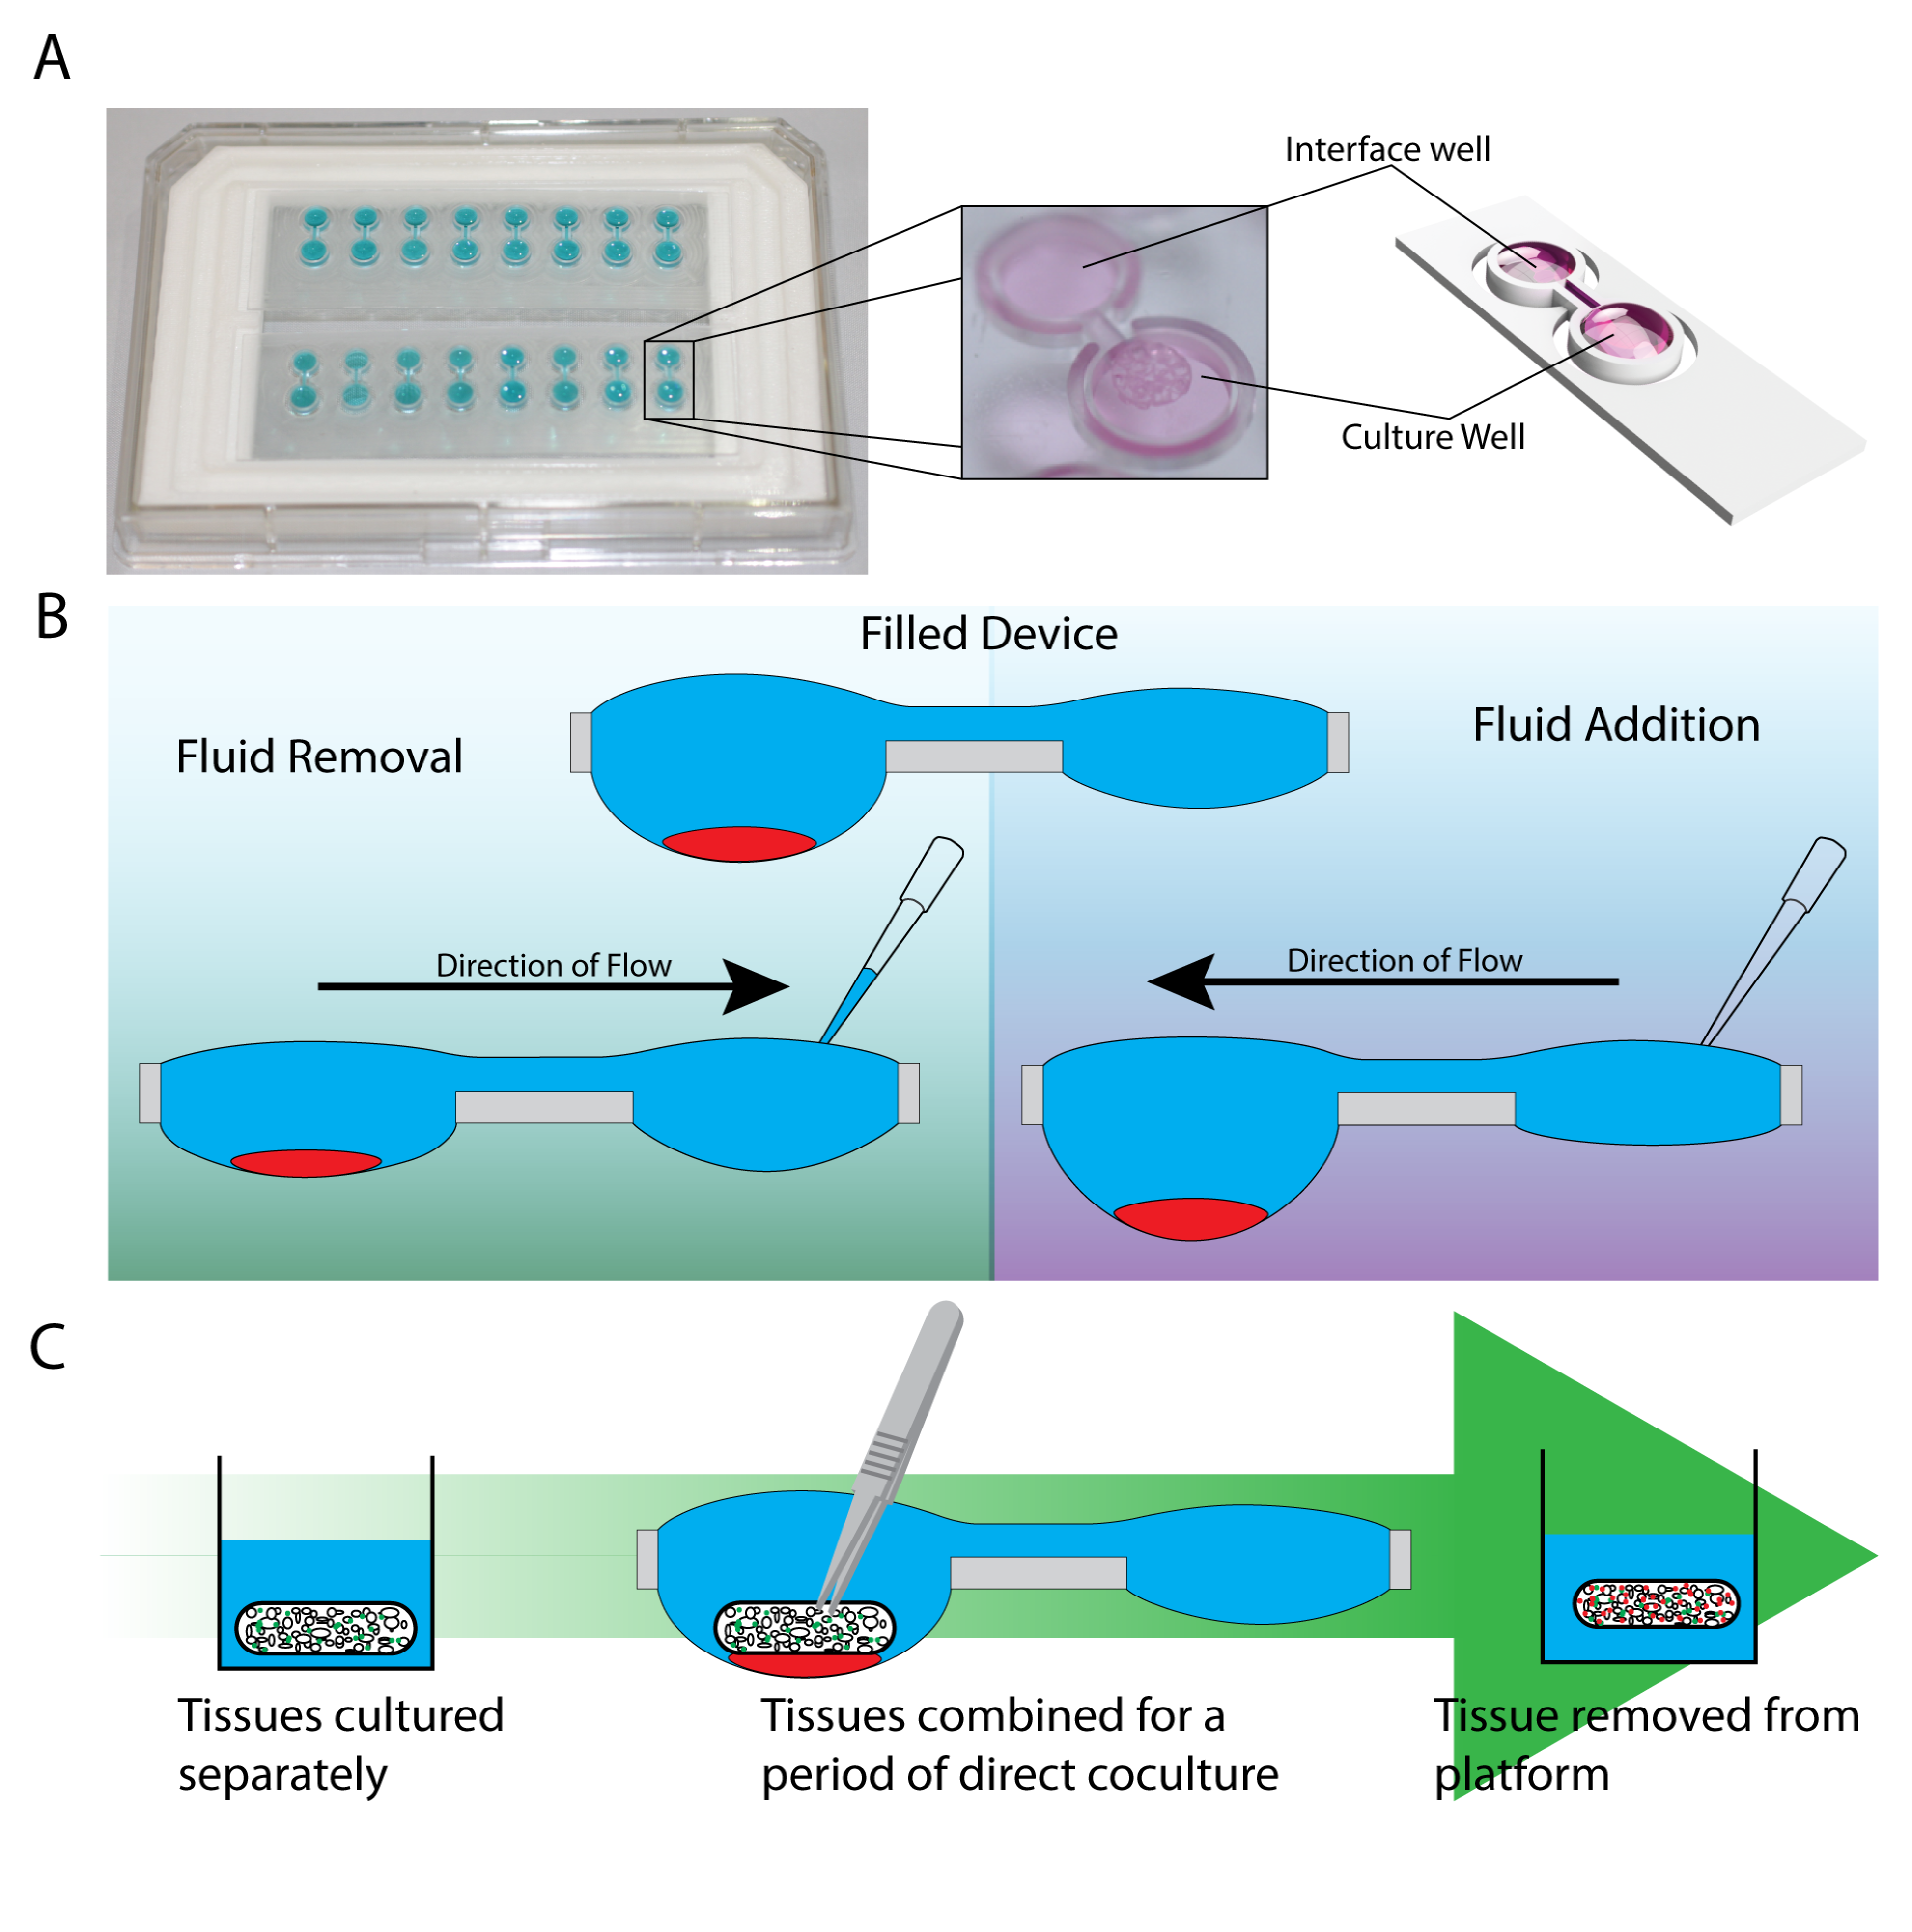
\includegraphics[width=5.4in]{/Figure1-RSC.png}
\caption[\textbf{The two-well hanging droplet device, operation, and capabilities}]{\textbf{The two-well hanging droplet device, operation, and capabilities}. (A) Two 8- device arrays of the two-well hanging droplet device with a close-up image and rendered-model of a single device. (B) Operation of a filled device containing cells, when fluid is removed or added through the interface well, volume of the culture well is changed with minimal disturbance to the culture. (C) Schematic of a dynamic coculutre experiment performed by combining two tissues in the hanging droplet device then separating the tissues.}
\label{figure:Fig1}
\end{figure}


\subsection{Characterization and modeling of two-droplet system}
We developed a numerical model for the behavior of the connected two droplet system to understand the limitations of the system, improve the functionality of the system, and guide the design of suspended droplet systems. The model predicts the distribution of fluid between two droplets as fluid is added or removed from the system. These predicted values were compared to values experimentally acquired in the device (Fig. \ref{figure:Fig2}Ai). Having a range of well characterized values allows the operation of the device with volumes that are robust and do not risk potential modes of failure. At low volumes, the hanging drop follows a surface-tension dominant regime dictated by the Laplace pressure \cite{Walker2002, Berthier2007} in which the two drops are close in volume. At higher volumes, however, gravity is non negligible, and the shape of the drop becomes elongated \cite{Carvajal2011}. Fluid distribution between wells at increasing volumes is illustrated in Figure \ref{figure:Fig2}Aii where the modeled fluid borders of each well at each volume is overlaid on images of the device. 

To predict the behavior of the system during device operation, we created a dynamic model of the device (Fig. \ref{figure:Fig2}B). With the model, we are able to observe that when one of the droplets, typically the droplet in the largest suspended port, becomes the lowest pressure region it acquires the majority of the liquid in the system. The model further shows that adding and removing fluid to the small drop results in approximately the same volume being shuttled to the well containing the largest drop. Importantly, this model validates the use of the small drop as a buffer for fluid additions; the small drop temporarily stores the fluid that was added by pipetting, prior to delivering it to the larger drop. Utilizing this approach, it becomes simple to tailor the delivery rate to the large drop in order to prevent excessive flow by designing the geometry of the channel connecting the two drops appropriately \cite{Berthier2011}. Finally, the model incorporates the dripping volume for a hanging drop, allowing the prediction of the maximum volume that can be added before detachment of the large drop. Alternatively, this can be utilized as a method for collecting the cellular sample; precise volumes of fluid can be added to cause the dripping of the cells in the drop into a receptacle placed below.

\begin{figure}[h!] %DONE
\centering
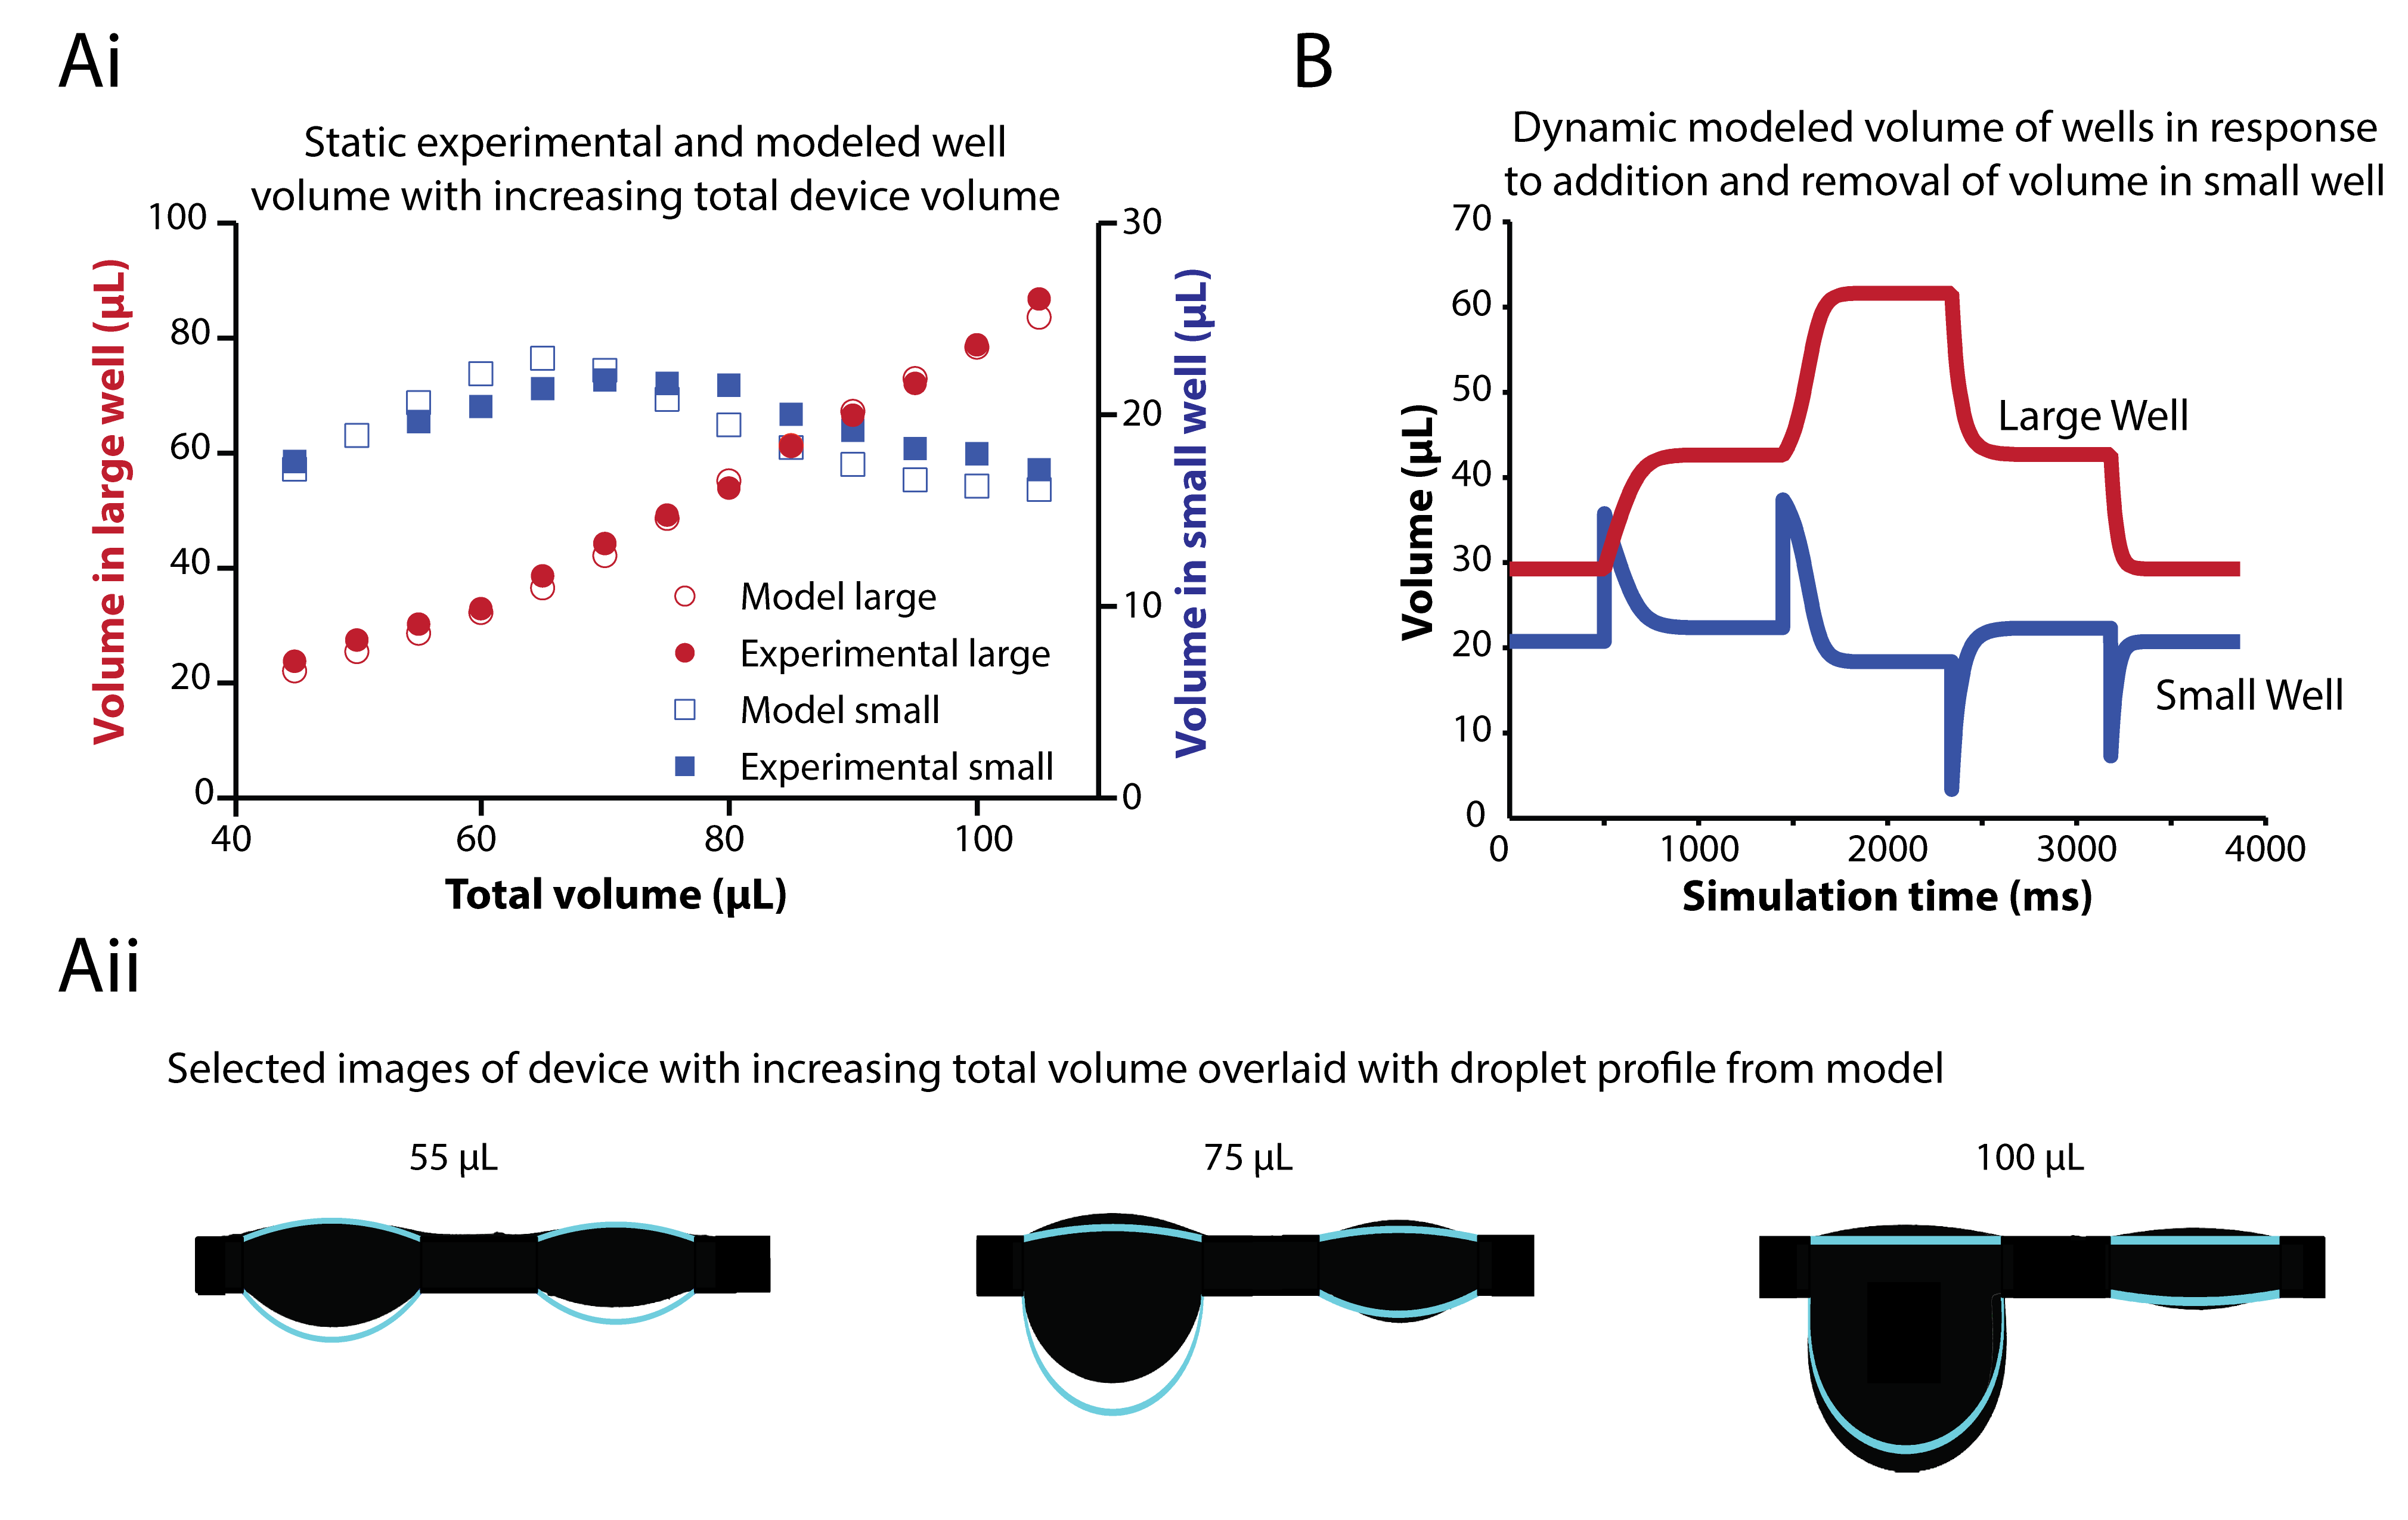
\includegraphics[width=5.75in]{/Figure2-rsc-01.png}
\caption[\textbf{Static and dynamic modeling of volume in each well of the device.}]{\textbf{Static and dynamic modeling of volume in each well of the device.} (Ai) The experimental (solid) and modeled (hollow) volume in each well at steady state with increasing total volume in the device. (Aii) The silhouetted device overlaid with the droplet borders of the modeled system for 55, 75, and 100 μL of total fluid in device. (B) Dynamic modeling of fluid in each well of the device as fluid is added then removed from the small well.}
\label{figure:Fig2}
\end{figure}


\subsection{Two-well hanging drop system prevents shear stress during media exchange}
Shear stress on a cell results in considerable changes to cell behavior \cite{White2007}, including inhibition of apoptosis in some cells \cite{Dimmeler1996} and induced proliferation and differentiation in other types \cite{Yamamoto2003}. In spheroid culture shear can prevent aggregation and completely disrupt the macrostructure of suspension cell cultures. Reducing shear experienced by cells in culture is critical to minimizing undesirable cell stimuli and achieving consistency between experiments. The two-well system provides a reduction in shear stress when changing fluid in hanging droplets compared to a one-well system. We performed an experiment to determine the extent of protection provided by the damping effect for droplet equilibration observed in our model (Fig. \ref{figure:Fig2}). This is best illustrated by a direct comparison between the two- and one-well systems (Fig. \ref{figure:Fig3}). We chose a multiple myeloma suspension cell line, MM.1S (commonly used for multiple myeloma drug studies \cite{Greenstein2003, Tai2006, Azab2009}) for the comparison, because suspension cell lines are generally difficult to culture in microdevices and are easily removed by flow. When cultured in the hanging droplet platform, MM.1S cells settle into clusters but do not form sphereoids. Addition or removal of fluid will result in loss of myeloma cells since the cluster is easily disturbed by minimal force exerted during fluid manipulation. In the hanging drop system media replacement is performed using iterative pipetting steps. Thus, we compared the performance of the two- and one-well systems over multiple pipetting steps.

We designed the experiment to ensure accurate comparison between the two- and one-well systems. The diameter and volume of the culture well in the two-well and one-well system was identical; the volume of fluid removed was based on a fraction (one third) of the total volume in each system. Pipetting was performed by a liquid handling robot to keep the flow rate constant. Each image in Figure \ref{figure:Fig3}A represents a different well subject to different conditions of fluid exchange, and all well images were collected within 10 minutes of pipetting. The two-well system protects cell clusters during fluid exchange after several pipetting steps, while pipetting into the one-well system results in immediate disruption of cluster morphology. These results combined with the data generated from computational modeling of the system underscore the need for an unequal two-well system for suspension cell culture to culture and retain cells to a single well, and suggest that media exchanges in one-well systems may have unintended effects on suspension cell culture.

To evaluate the difference in shear between pipetting into a single-well versus a two-well system, we performed particle image velocimetry (PIV) analysis on fluorescent microbeads in the culture well (Fig. \ref{figure:Fig3}B). Fluid was added \textit{via} the user interface well (in the two-well system) or directly into the culture well containing the fluorescent beads (in the one-well system). There was a 10-fold reduction in the velocity of beads in the two-well device compared to the single-well one. This reduction velocity corresponds to a comparable decrease in shear stress experienced by cells in the device. Furthermore, the reduction in velocity in the two-well system enables quicker media changes without cell disruption, compensates for variation of users operating the device manually, and results in shorter times where the device needs to be exposed (to interface with pipettes), reducing potential evaporation.

\begin{figure}[h!] %DONE
\centering
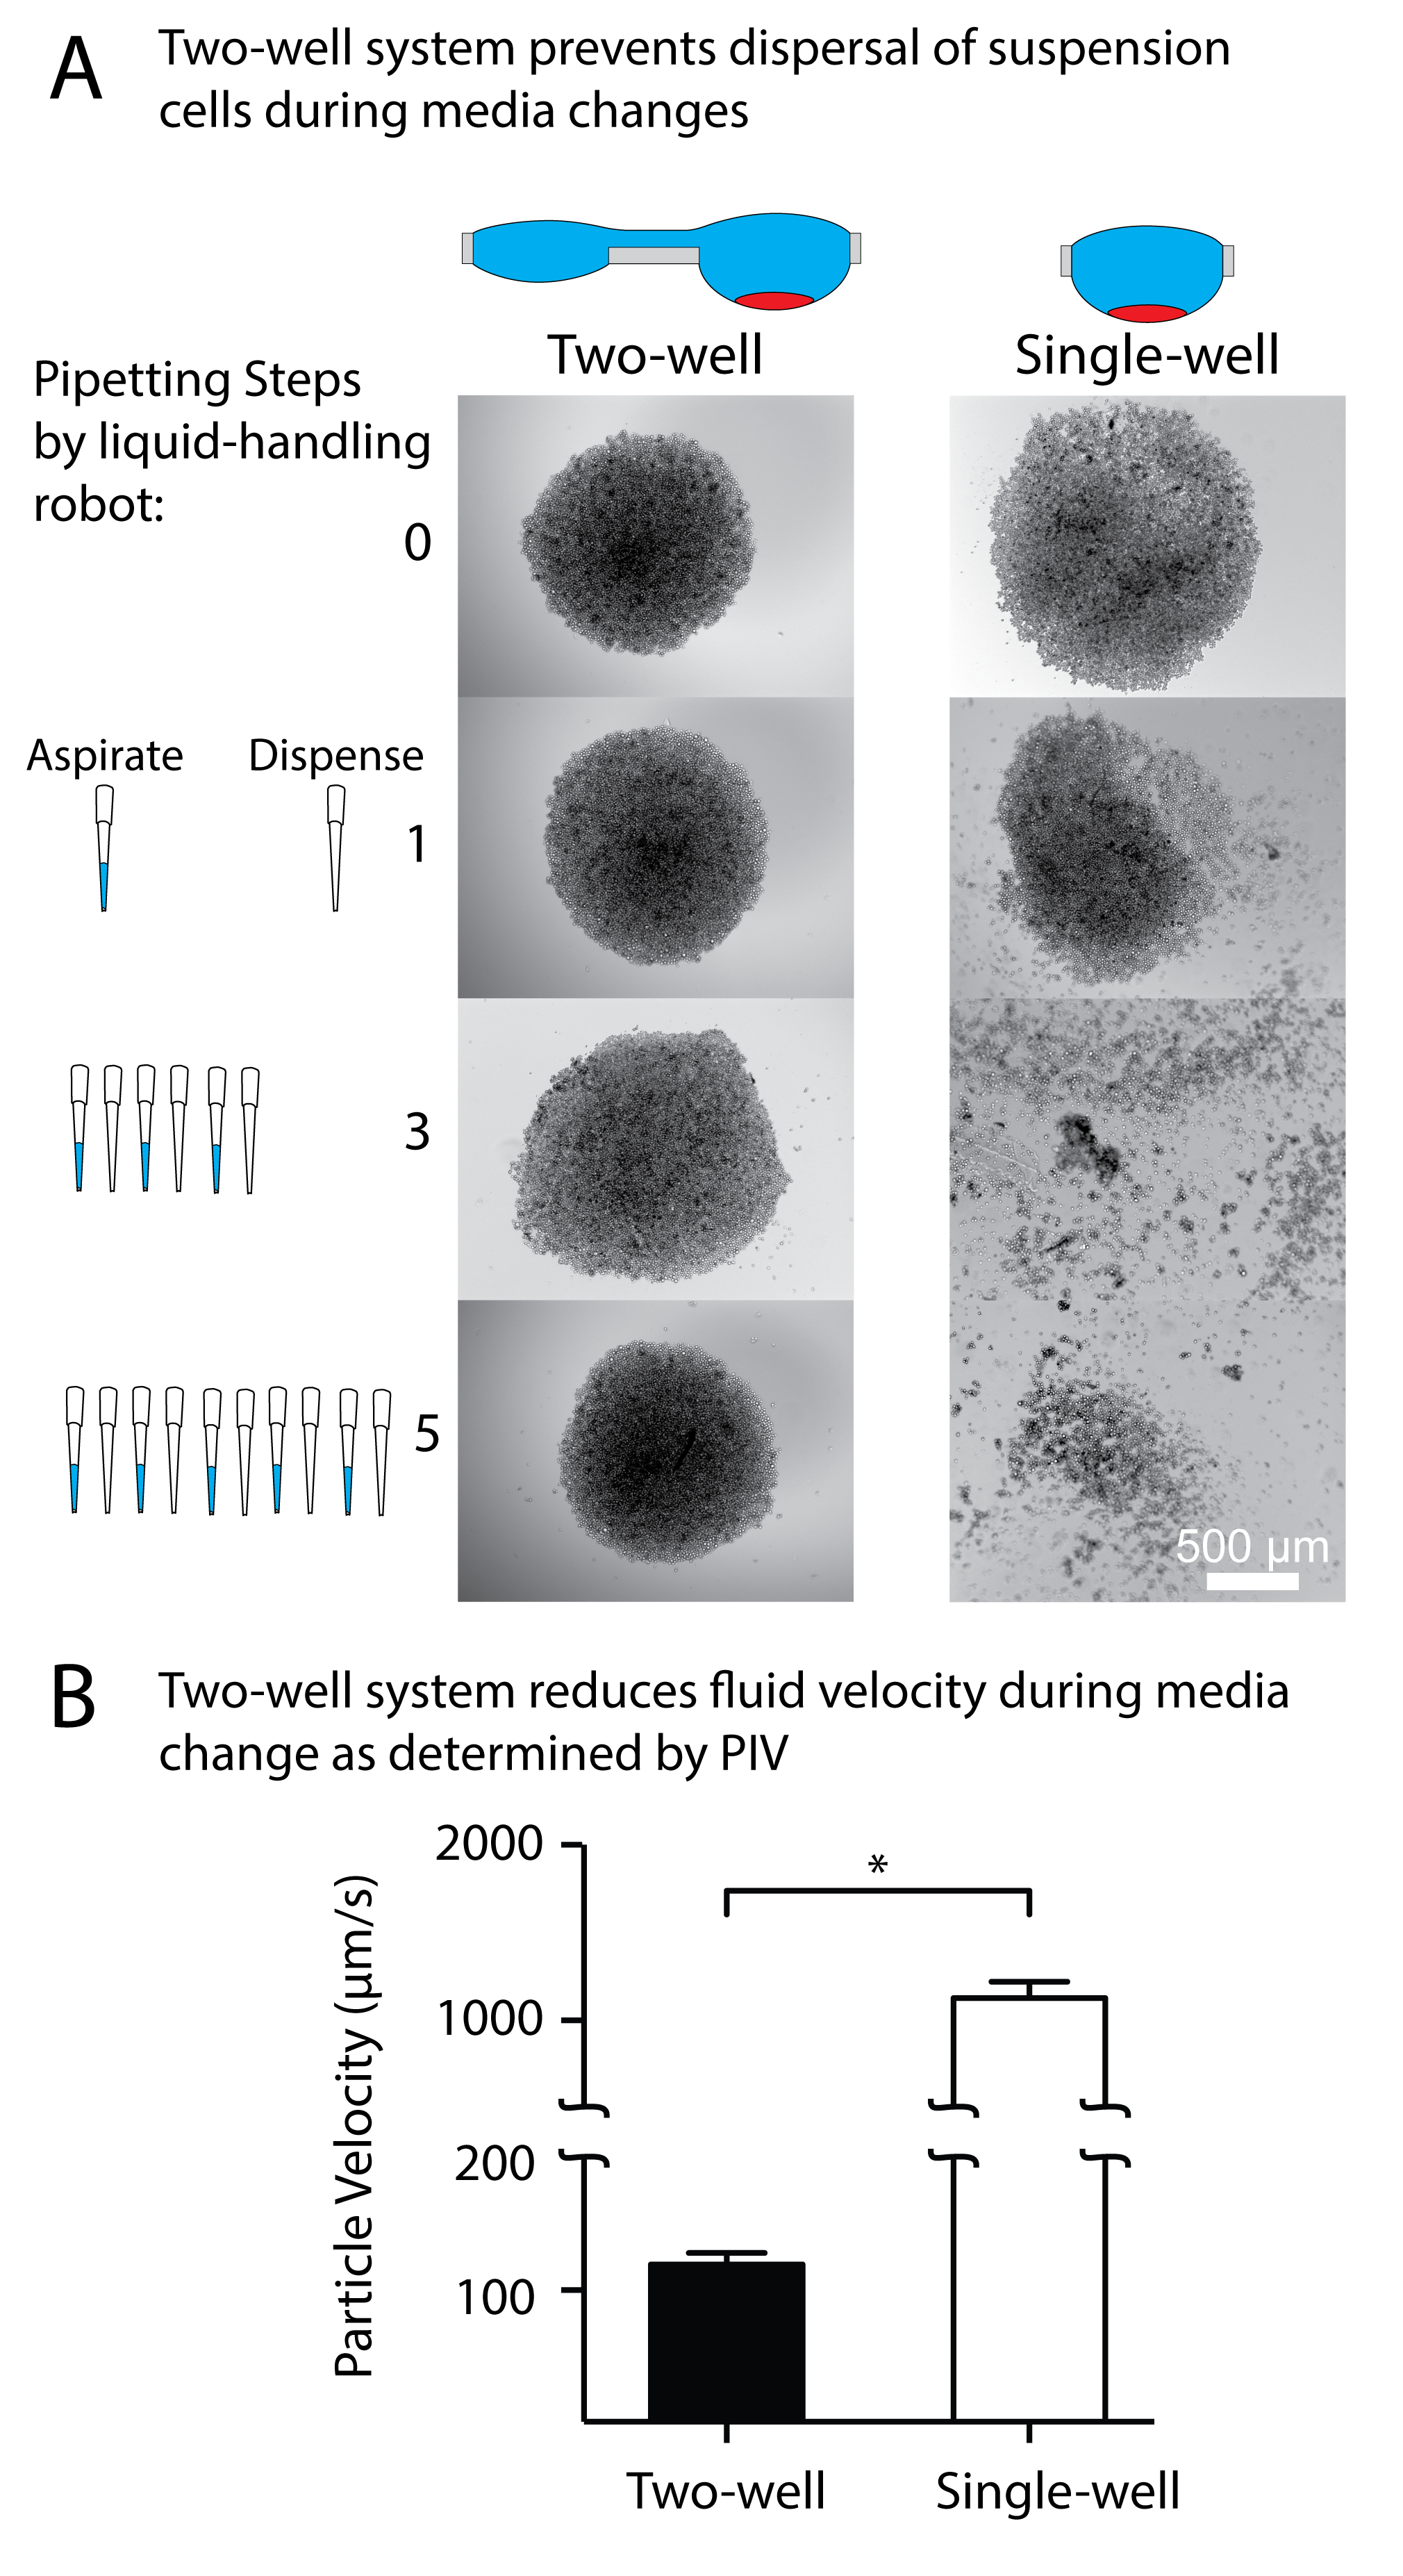
\includegraphics[width=3in]{/Figure3-RSC.png}
\caption[\textbf{Effects of pipetting into a single-well and two-well device}]{\textbf{Effects of pipetting into a single-well and two-well device.} (A) Brightfield images of an MM.1S suspension culture in the device before and following 1, 3, and 5 pipetting steps at 1 mL/min of approximately 33\% of the total media in single-well and two-well device. (B) PIV was used to determine the velocity of fluid at a fixed z position in the culture droplet during fluid addition to the interface droplet (two-well) or directly (single-well). Error bars represent the standard deviation of four replicates (*p<0.0001).}
\label{figure:Fig3}
\end{figure}

\subsection{Open hanging droplet platform facilitates key cell culture manipulations and readouts}
For functional validation, we demonstrated that the hanging droplet culture platform is well suited to perform functions critical for tissue culture, experimentation, and analysis: long-term culture, ability to apply treatment, and immunocytostaining. We chose to focus our cellular validation experiments using suspension (or non-adherent) multiple myeloma cells. Multiple myeloma is the second most common hematopoietic malignancy in the United States, and has a 47\% median 5-year survival rate. Multiple myeloma affects its microenvironment through a complex network of interactions with surrounding matrix and cells resulting in the destruction of healthy bone \cite{Reagan2014} and acquisition of drug resistance \cite{Bianchi2006}. The fact that multiple myeloma cells are non-adherent precludes the use of many currently available microculture platforms for studying the disease.  We performed the platform validation using the multiple myeloma cell line, MM.1S. The MM.1S cell line is an important model for multiple myeloma, and the assays we have focused on are key to studying the disease and patient-specific drug responses \cite{Young2012}.
\newline
\textit{i. Long term culture.} The extended culture experiments were performed over the course of 9 days, feeding the culture every other day through media replacements, resulting in approximately 75\% new media in the culture well each feeding. The MM.1S cells expressed mCherry, which was used to perform a relative quantification of total cells in the well. Mean integrated density of fluorescence signal across the entire well was used because a single cell count was not feasible due to the high density of cells and cell-to-cell variation in mCherry expression levels. Over the course of the experiment (Fig. \ref{figure:Fig4} A), the number of cells increased through day 5, but had stopped by the 6th day. At that time in the culture, the wells had become overpopulated resulting in stagnation of the mean integrated density. Though nine-day culture is rarely required for common experiments such as drug screens, we have demonstrated the practicality of long-term culture in the device. \newline
\textit{ii. Cell viability in response to \textit{in situ} treatment.}

We characterized growth inhibition of the culture in response to a drug to demonstrate the ability to apply treatments during culture and measure a dose-response. We treated MM.1S cells with bortezomib, a proteasome inhibitor and commonly used treatment for multiple myeloma (Fig. \ref{figure:Fig4}B). The IC50 value of the MM.1S culture in response to bortezomib was determined to be 26.2 nM with an R\textsuperscript{2} of 0.84. The previously reported IC50s of bortezomib for the MM.1S cell line typically range between 4 and 9 nM \cite{Bianchi2006, Hu2014, Horton2006}, but these values were all calculated in 2D culture. It has been widely shown that 3D culture conditions often decrease drug sensitivity \cite{Tung2011, Friedrich2009}and better recapitulate in vivo response. The calculated response also for a 24 hour exposure time, follows a distinct 4 parameter logistic sigmoidal curve characteristic of inhibitory dose-response curves. 

\textit{iii. High content assays and immunocytochemistry (ICC)} To establish the viability of functional readouts in the platform, we characterized NF-\textkappa B translocation to the nucleus in MM.1S cells in response to stimulation \textit{via} TNF-\textalpha. Quantifying translocation of factors between cell membrane, cytoplasm, and nucleus of the cell provides a high-content assay that can give information about the state of a single cell or population of cells. Translocation of factors around the cell is a vital component in cell behavior and proliferation \cite{Chuderland2008}. Misregulation of translocated factors, such as estrogen receptor in breast cancer \cite{Revankar2005} and androgen receptor in prostate cancer \cite{Molina2011}, contributes to treatment resistance. In multiple myeloma, NF-\textkappa B has been implicated as key regulator of inflammation, cancer progression, cell survival, and acquired resistance \cite{hideshima2000thalidomide}, and thus is considered as a potential therapeutic target. 

We performed an experiment to induce translocation of NF-\textkappa B in response to TNF-\textalpha  in the MM.1S cell line (Fig. \ref{figure:Fig4}C). TNF-\textalpha  is expected to cause NF-\textkappa B to translocate to the nucleus following treatment and is the first step in the transcription of a number of pro-inflammatory mediators \cite{Pahl1999}. Translocation is indicated by a steeper slope in the scatter plot comparing the mean signal intensity of NF-\textkappa B in the nucleus versus the cytoplasm (Fig. \ref{figure:Fig4}Ci). When considering the entire population of cells using a histogram, a population-wide increase in translocation is visualized as a shift to the right on the x-axis (mean nuclear NF-\textkappa B signal intensity to mean cytoplasmic NF-\textkappa B signal intensity) with a median shift from 1.0 in the untreated condition to 1.2 in the treated conditions with p<0.001 from analysis with the Mann-Whitney U test for 4 replicates (Fig. \ref{figure:Fig4}Cii).

\begin{figure}[h!] %DONE
\centering
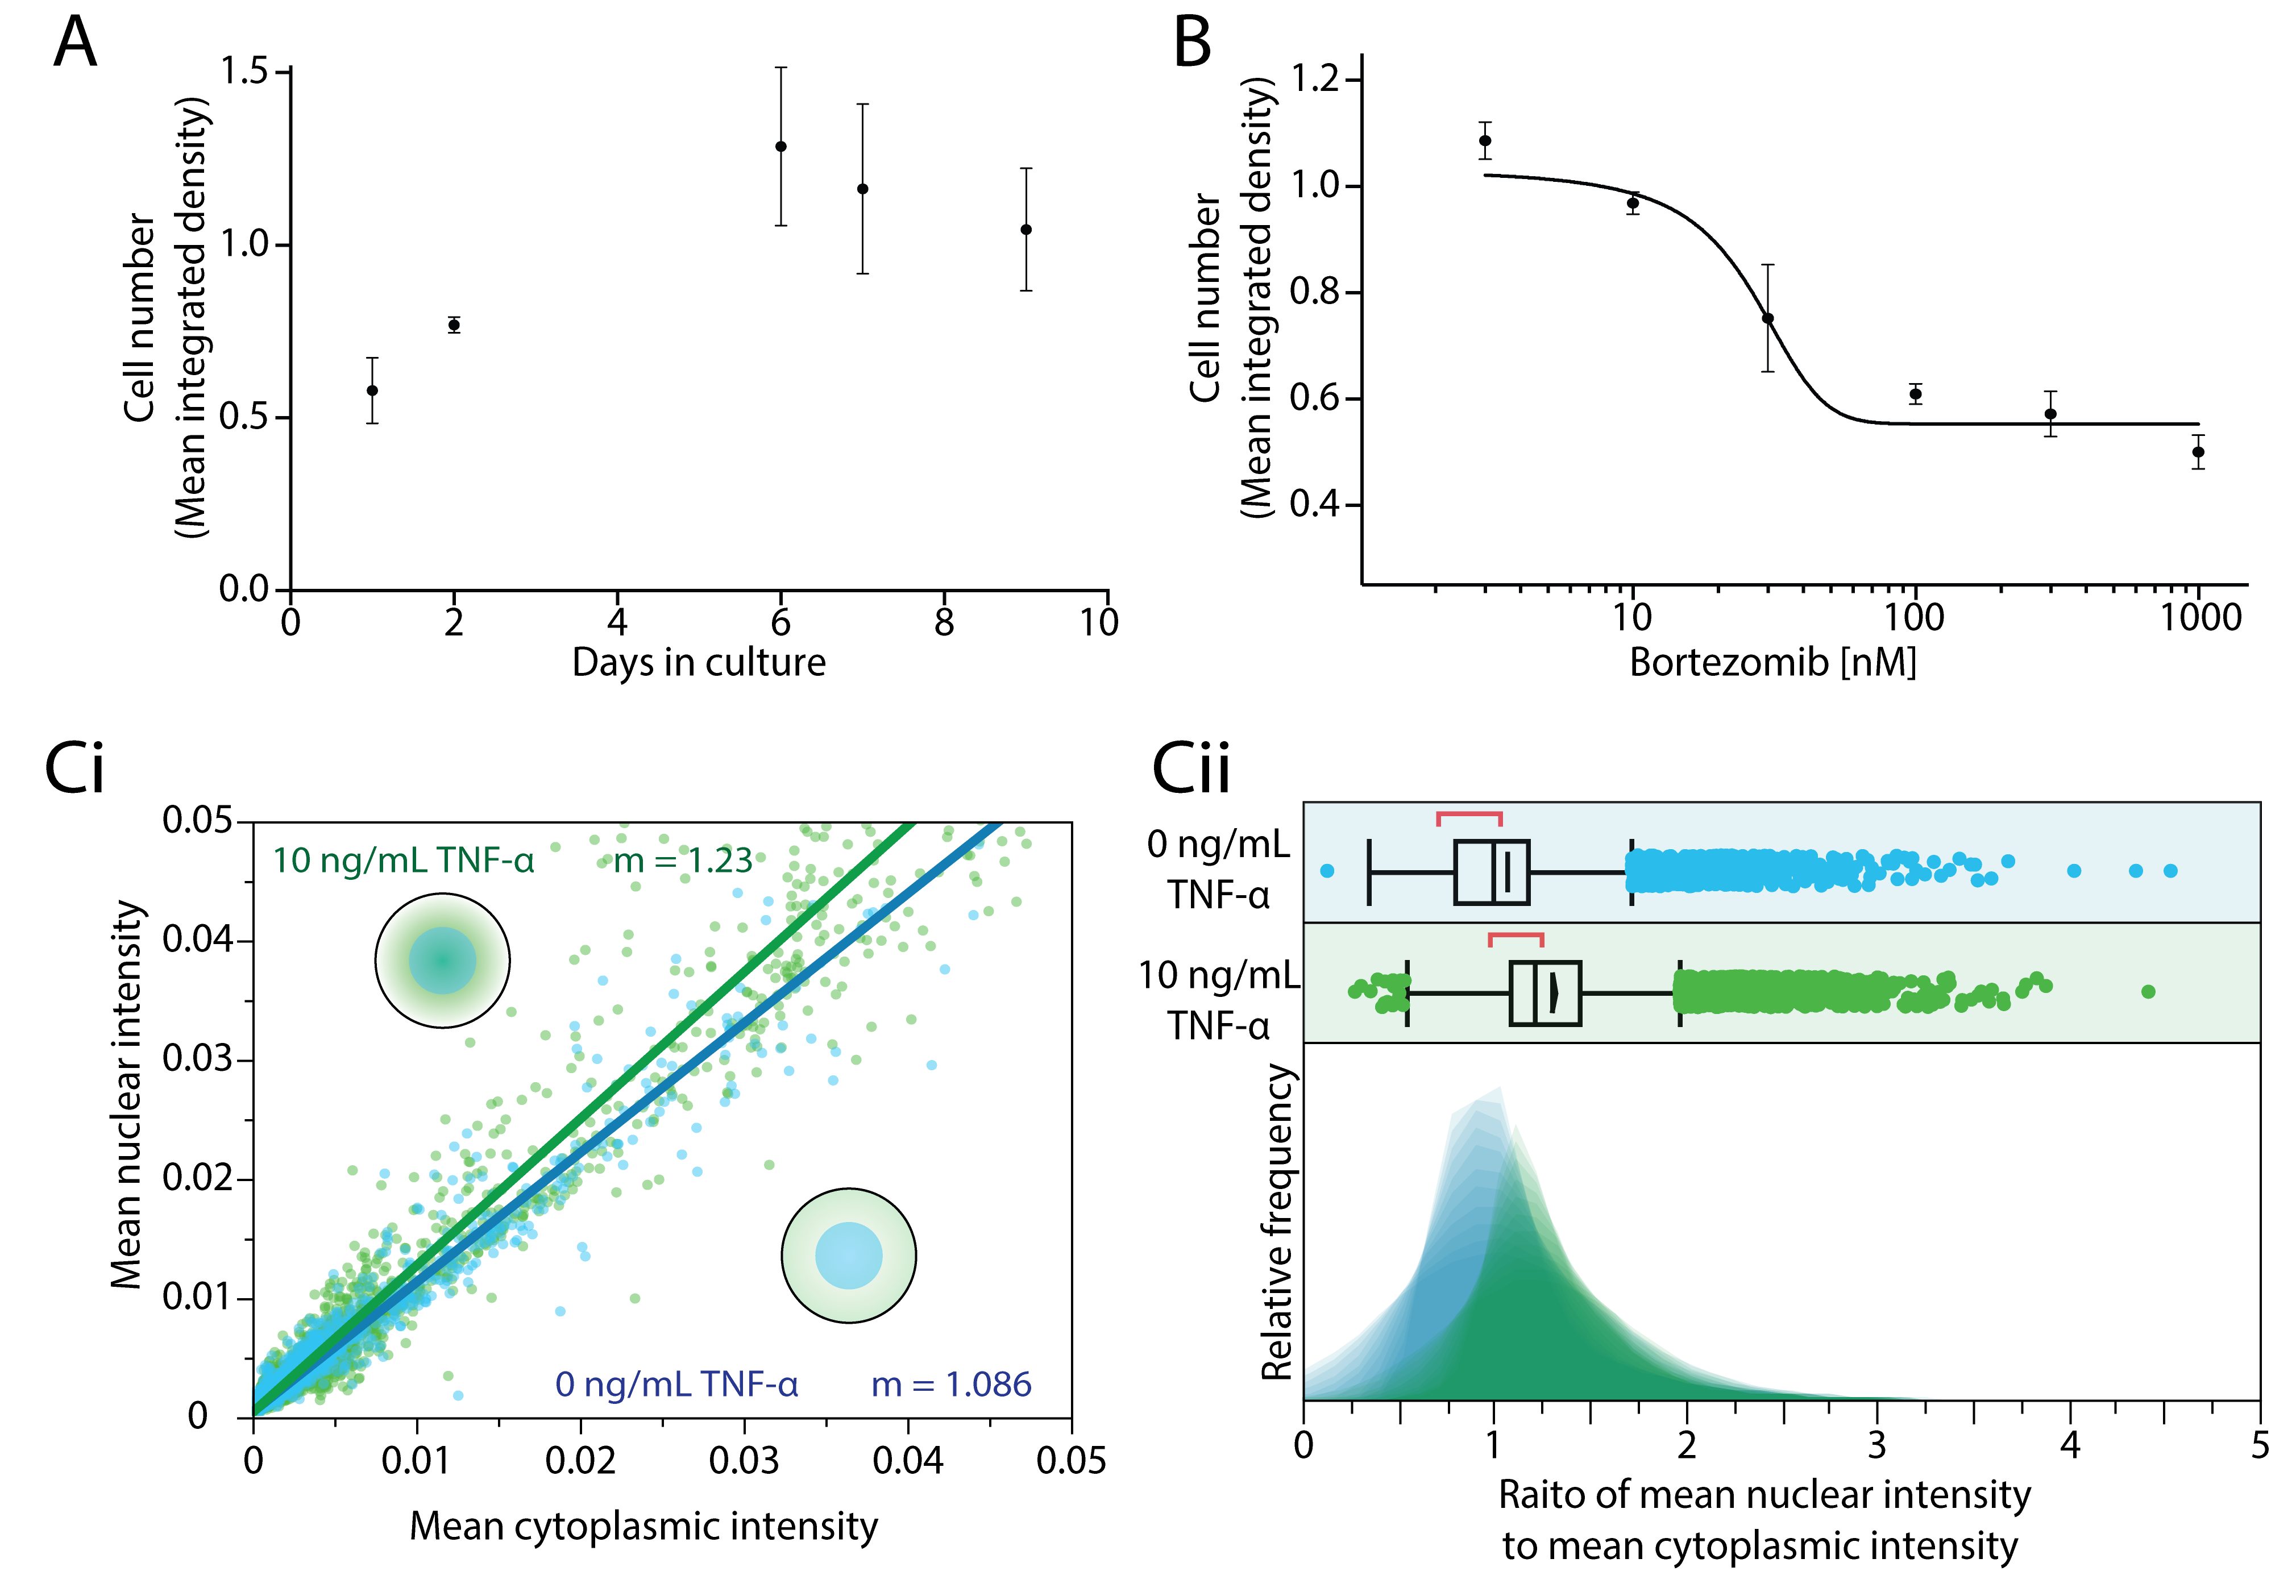
\includegraphics[width=5.75in]{/Figure4-RSC.png}
\caption[\textbf{Open hanging droplet platform facilitates key cell culture manipulations and readouts.}]{\textbf{Open hanging droplet platform facilitates key cell culture manipulations and readouts.} (A) Long term culture: Growth of MM.1S cells in device across a 9-day culture. Error bars represent the standard error of the mean (SEM) of 7 wells. (B) Cell viability assays in response to in situ treatment: Growth inhibition response curve of MM.1S cells to increasing concentrations of bortezomib in culture. Error bars represent the SEM of 5 wells. (C) Characterization NF-\textkappa B nuclear translocation in MM.1S cells following treatment with 10 ng/mL of TNF-\textalpha \, (green) or no treatment (blue). (Ci) Scatter plot of mean nuclear intensity versus mean cytoplasmic intensity. (Cii) Histograms of the ratio of mean nuclear intensity to mean cytoplasmic intensity for the population of cells.}
\label{figure:Fig4}
\end{figure}

For the NF-\textkappa B translocation assay described above, we developed methods to perform ICC on cells from hanging drop cultures. We first attempted to perform ICC in situ (i.e., in the hanging droplet device), leveraging the two-well system to exchange ICC reagents. However, performing ICC requires a permeabilization step using surfactants, which inherently reduce interfacial tension. Standard in situ ICC was found to be incompatible with the hanging droplet device due to the reliance on pressure equilibration to move fluid between wells. When surfactant is added to the user interface well  the surface tension decreases, causing a shuttling of fluid from the culture well into the interface well. To achieve high-content ICC in the NF-\textkappa B translocation assay, we instead transferred the cells from the hanging droplet wells to a poly-L-lysine-treated slide to retain cells during fluid exchange by touching off the droplets onto the surface of the slide.  Performing ICC and imaging on plated cells has several advantages compared to in situ ICC and imaging. The cells are spread throughout the plate, allowing for better separation of cells and therefore better characterization of single cells to be achieved. Plating cells also enables higher objectives to be used for imaging and longer imaging times to be achieved. In the current configuration, devices would need to be removed from the humidifying dish to be accessed by high magnification objectives due to working distance limitations. 

It is worth noting that other staining protocols that do not require surfactants, such as live/dead assays, can be performed directly in the hanging droplet device. We demonstrated this using the adherent cell line MDA-MB231, which forms spheroids in hanging droplet culture (Fig. \ref{figure:FigS2}). We incubated the device in both normoxic and hypoxic conditions to study the spatial distribution of live and dead cells within the spheroid. Live/dead staining was performed within the hanging droplet device, and the spheroids were removed for imaging (Fig. \ref{figure:FigS2}). 
\newline
\textit{iv. Culture treatment, media sampling and cytokine quantification}The ability to sample and analyze media throughout the course of an experiment without disturbing the culture is powerful for studying progression of a culture system. The two-well system is well-suited for media collection and treatment addition through the interface well. To validate the platform for treatment and sampling, we cultured a polymeric porous bone-like scaffold seeded with bone marrow stromal cells in the device. The scaffolds were treated at seeding and after 24 hours with AMD3100, an inhibitor of CXCR4, indicated in homing and adhesion for cells to the bone marrow microenvironment \cite{Alsayed2007, Burger2006}. The media was sampled at 24 and 48 hours from the interface port and analyzed for the pro-inflammatory, IL-6 cytokine indicated in microenvironment-mediated drug resistance and a number of pro-tumorigenic pathways \cite{Hodge2005, Roodman2001a, Vincent2005, Lin2007}. IL-6 was detected in both the control and AMD3100-positive conditions when sampled from the interface well (Fig. \ref{figure:Fig5}A). As expected, we observed a trend toward reduced IL-6 secretion with AMD3100 treatment. This experiment demonstrates that cytokines secreted by cells in the culture well are able to be detected in the interface well and suggests that this device could provide a useful tool for conducting soluble factor signaling-based coculture experiments using more complex culture constructs. We further evaluated soluble factor exchange in the device through computational modeling of diffusion in the system starting with an initial concentration of a molecule with similar diffusion properties to IL-6 in the volume occupied by the bone-like scaffolds (Fig. \ref{figure:Fig5}B). At 4 hours, the diffusion gradient stabilizes within the culture well of the device creating a pattern where the culture well has a stable "high" concentration and the interface well have a stable "low" concentration of the solute. Further characterization of diffusion within the device is available in the ESI (Fig. \ref{figure:FigS3}).    

\begin{figure}[h!] %DONE
\centering
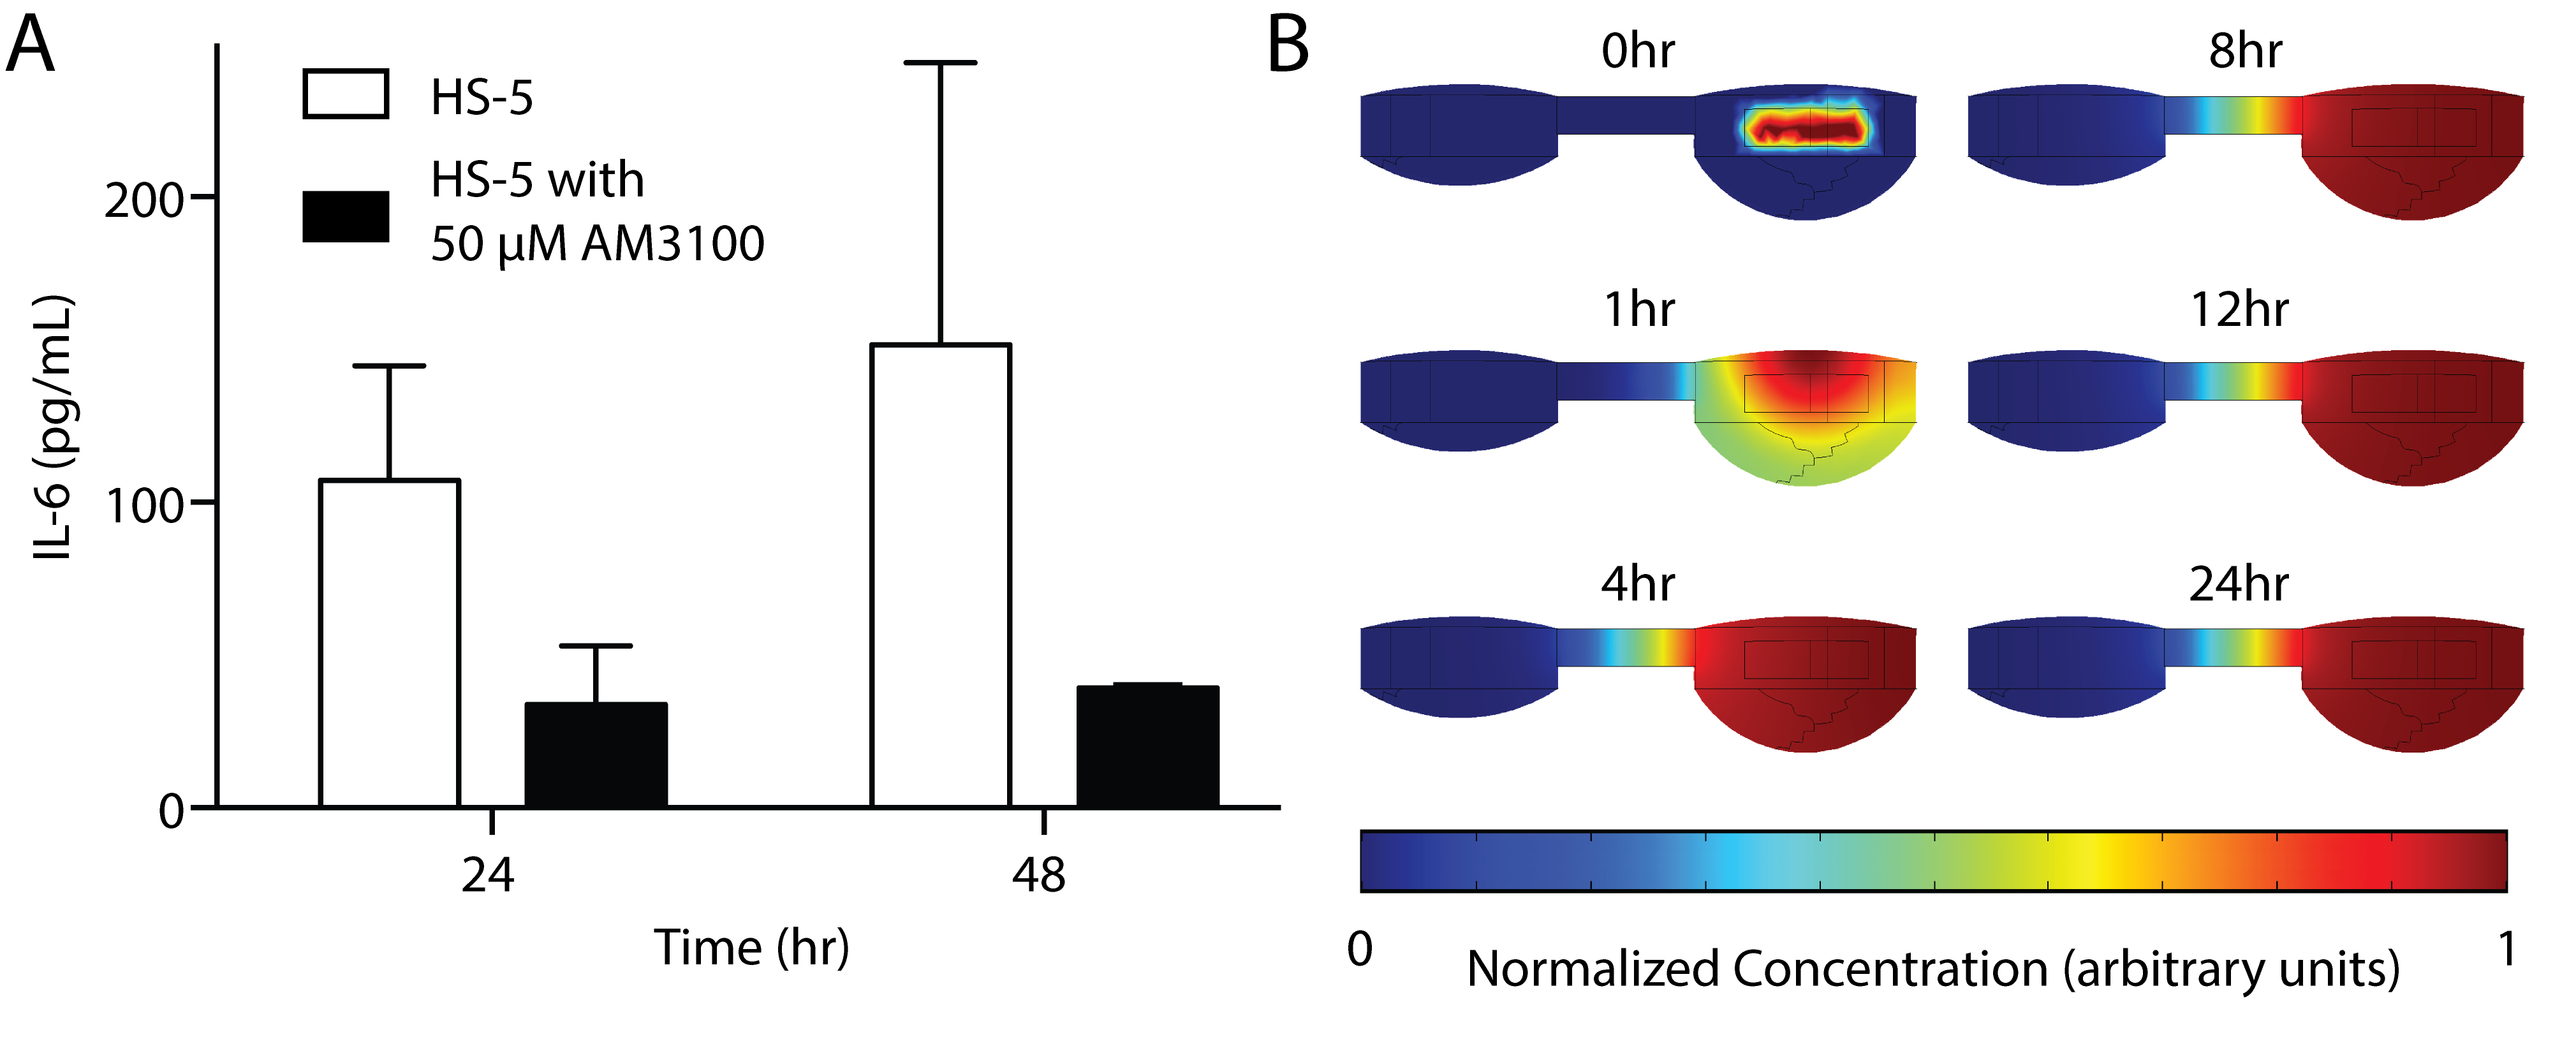
\includegraphics[width=5.75in]{/Figure5-RSC.png}
\caption[\textbf{Soluble factors in culture.}]{\textbf{Soluble factors in culture.} (A) Concentration of IL-6 isolated from HS-5-seeded bone-like scaffolds cultured in device taken from the interface well at 24 and 48 hours of culture. Error bars represent the SEM of 3-4 wells. (B) Plot of normalized concentration for simulated diffusion in the device at several time points over 24 hours. The initial concentration of solute was localized to the volume occupied by the bone-like scaffold at time = 0 h. The solute simulated was approximately 10 kDa with a diffusion coefficient of 100 \textmu m\textsuperscript{2}/s.}
\label{figure:Fig5}
\end{figure}


\subsection{Dynamic culture of cells and tissue scaffolds}
The geometry of the device allows for direct access to the culture through the open wells. This access can be exploited to manipulate culture throughout the course of an experiment. We demonstrated manipulation of the media through the wells (sections 3.3 and 3.4), importantly, the open system facilitates interaction beyond simple media changes and liquid treatments. As shown in Fig. \ref{figure:Fig1}, tissue scaffolds and solid objects can be introduced \textit{via} direct access to the culture well (e.g., by using tweezers to place the scaffold in the open device). To explore the ability to manipulate tissue throughout the course of an experiment, we performed a coculture of multiple myeloma and bone marrow stromal cells (BMSCs). BMSCs play an important role in multiple myeloma progression and provide the tumor with protection against treatment \cite{Chauhan1996, Chatterjee2002a}. Adhesion of multiple myeloma cells to the stroma is an important step in disease progression as non-malignant B-cells have very low capacity for adhesion \cite{Tai2006}.

We began the culture separately, with BMSCs in polymeric, porous, bone-like scaffolds and myeloma seeded into wells in the hanging droplet device. The cultures were combined in the hanging droplet device and myeloma cells were allowed to migrate into the scaffold. The scaffolds were removed for imaging following coculture and adhesion of MM.1S cells was characterized (Fig. \ref{figure:Fig6}). Adhesion of the MM.1S cells to the scaffold was seen in both direct coculture, where the scaffold and MM.1S cluster were in the same well, as well as in the blank scaffold MM.1S monoculture condition. MM.1S cells were not detectable in either BMSC monoculture or separate coculture. These results enable us to explore the impact of the multiple myeloma microenvironment for both soluble factor signaling as well as cell-cell contact for tumor-stromal interactions. 

\begin{figure}[ht] %DONE
\centering
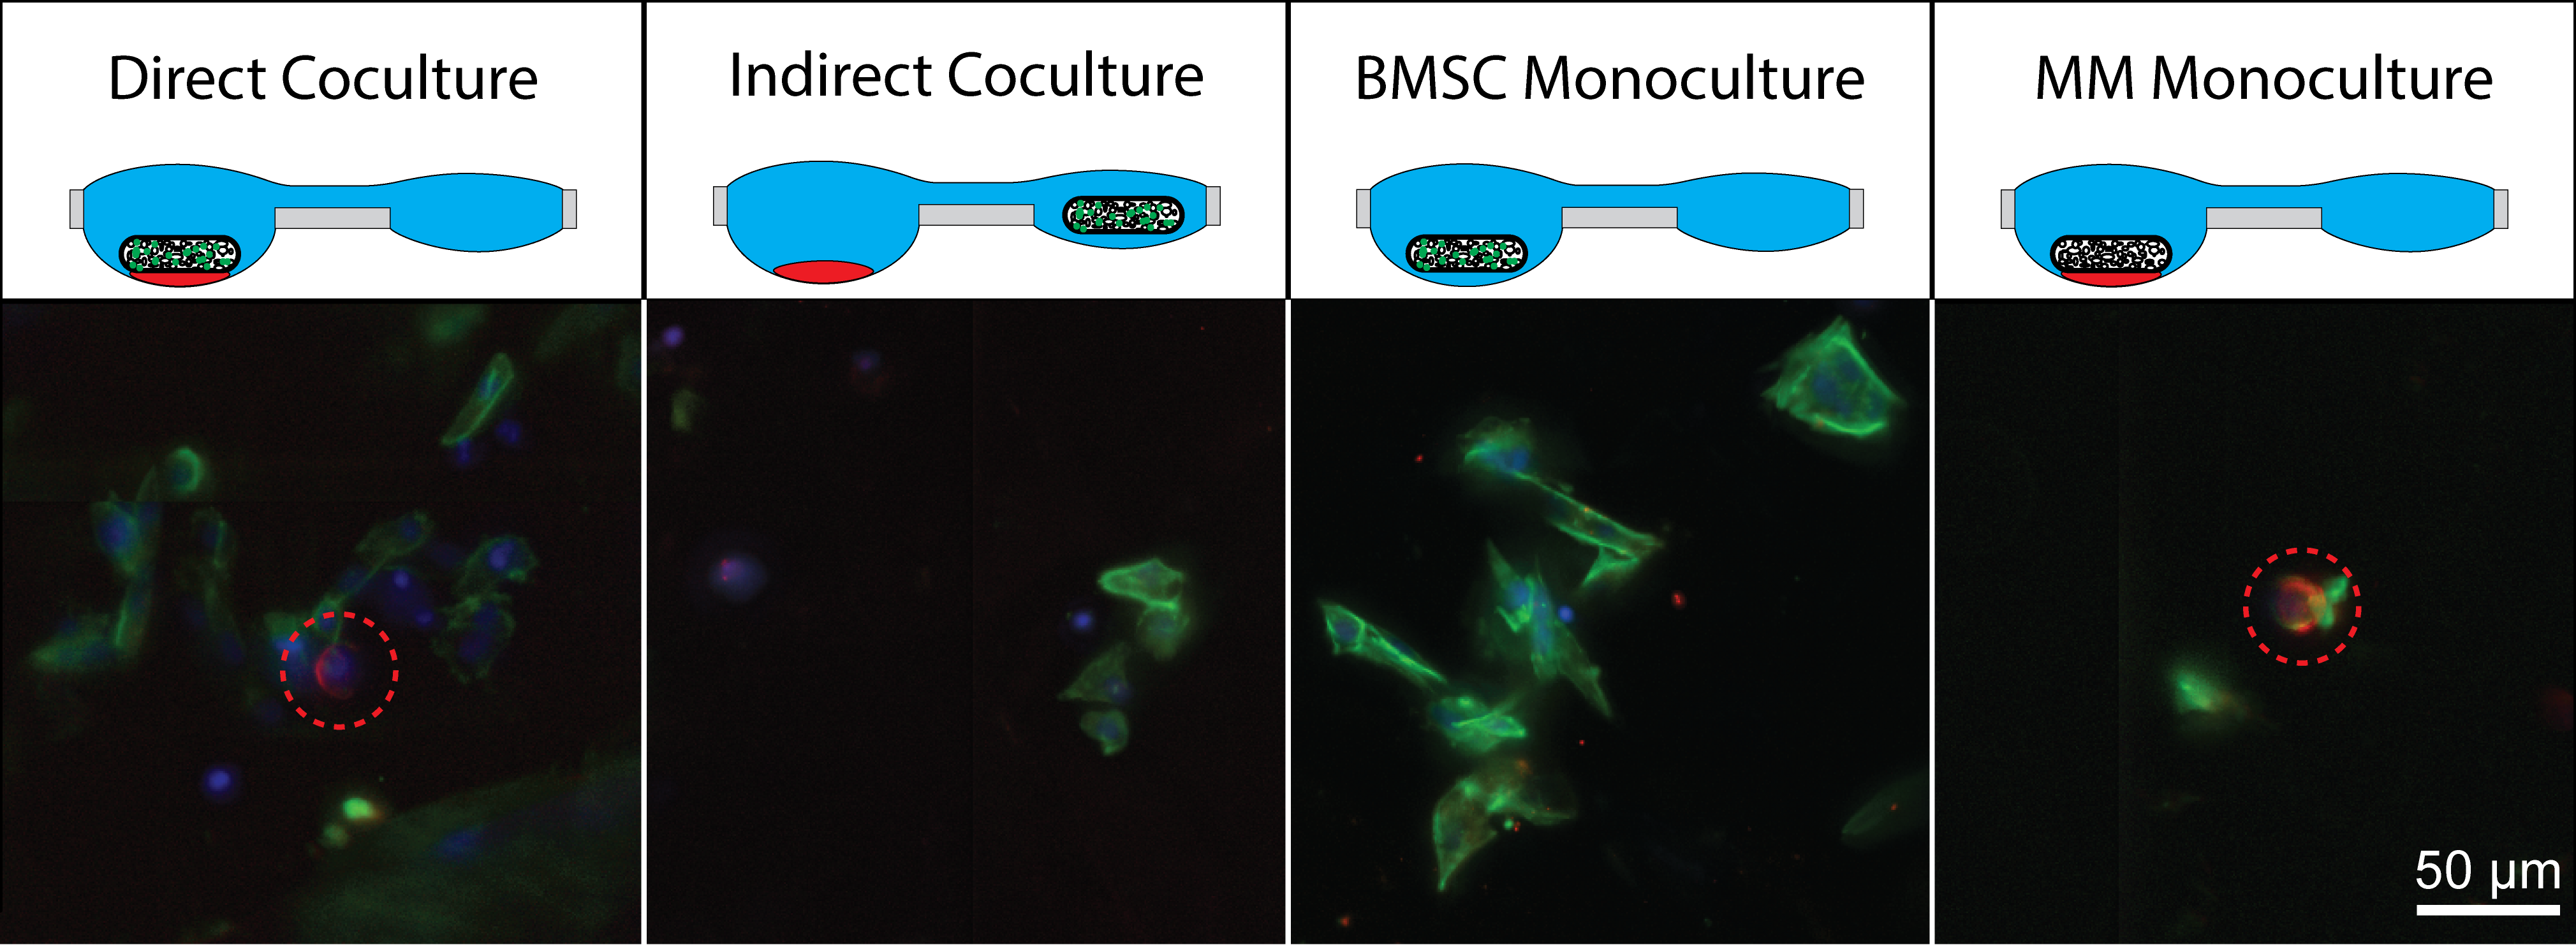
\includegraphics[width=5.5in]{/Figure6-RSC.png}
\caption[\textbf{Coculture and migrations of MM.1S cells into polymeric bone-like scaffold.}]{\textbf{Coculture and migrations of MM.1S cells into polymeric bone-like scaffold.} Fluorescent images of polymeric bone-like scaffolds following either direct coculture (BMSC-seeded scaffold with MM.1S cluster - same well), indirect coculture (BMSC-seeded scaffold with MM.1S - separate wells), BMSC monoculture (BMSC-seeded scaffold only), or multiple myeloma monoculture (MM.1S cultured with blank scaffold). BMSCs were identified by presence nuclear stain (blue) with actin (green), while MM.1S cells were identified by nuclear stain, actin, and CD138 ring (red) and highlighted with a red dotted circle.}
\label{figure:Fig6}
\end{figure}


\section{Conclusions}
We have developed an open platform that enables the dynamic culture and analysis of tissues in a hanging drop embodiment. We have demonstrated that an asymmetric two-well droplet system enables the long-term culture of shear-sensitive cells while allowing for the application of treatments over the course of an experiment. Leveraging the open surface of the hanging drop wells, we are able to add and remove tissue from the culture platform during the course of an experiment to enable dynamic coculture configurations, which are difficult to achieve in closed culture platforms and facilitates easy downstream analysis of cultures. The platform addresses challenges of culturing suspension cells in 3D culture as well as coculture with adherent cell types. The platform enables configurations of cells that were previously either unachievable or impractical, allowing for the investigation of new biological phenomena. We will continue to explore the biology enabled by this platform with the development of more complex biological tissues formed with step-wise, dynamic component addition. 

\section{Acknowledgements}
The authors would like to thank Drs. Shigeki Miyamoto and Fotis Asimakopoulos for their expertise and biological insight into multiple myeloma, Dr. William Murphy and Eric Nguyen for their contributions to in situ imaging in the  and bone marrow scaffold development, and Dr. Jay Warrick for his assistance in PIV analysis. This work was funded by University of Wisconsin Carbone Cancer Center Support Grant P30 CA014520 and National Institutes of health grants; NIH R01 CA155192 (D.J.B.), NIH T32HG002760 (T.E.d.G.), NIH K12 DK100022 (A.B.T.). T.d.G. has ownership in Stacks to the Future, LLC and Lynx Biosciences, LLC. E.B. has ownership in Stacks to the Future, LLC and Tasso, Inc.   D.J.B. has ownership in BellBrook Labs, LLC; Salus Discovery, LLC; Stacks to the Future, LLC; and Tasso, Inc. A.B.T. has ownership in Stacks to the Future, LLC.


%% Start the appendices:
\appendix       % Chapters, sections are now appendix style
\chapter{Surface-tension driven open microfluidic platform for hanging droplet culture}
\label{App:HangingDroplet}

\begin{figure}[ht] %DONE
\centering
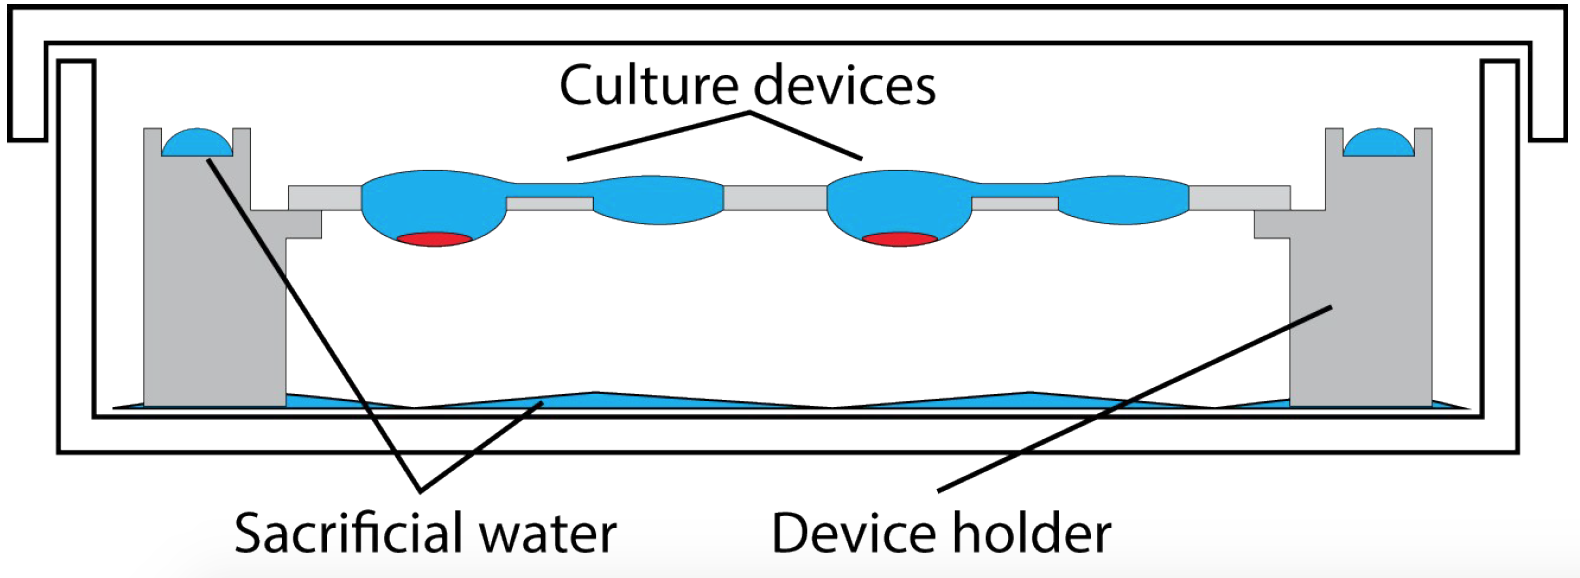
\includegraphics[width=4.5in]{/FigS1.png}
\caption{The device holder is placed in an OmniTray (Nunc) water is added to the bottom of the OmniTray and to the channel features of the device holder. The device is then placed into the device holder and filled with mediaand cells. The lid is placed on the OmniTray to ensure proper humidification of the device to prevent evaporation.}
\label{figure:FigS1}
\end{figure}

\begin{figure}[ht] %DONE
\centering
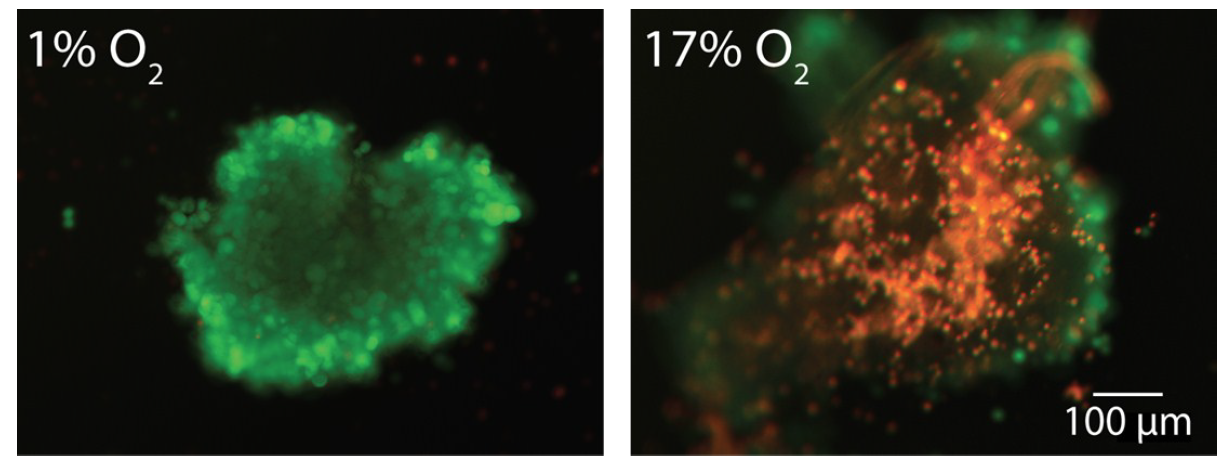
\includegraphics[width=4.5in]{/FigS2.png}
\caption{10,000 MDA-MB-231 cells were seeded into the culture well of the device and were cultured at either normoxic or hypoxic conditions for 48 hours before imaging. Live cells (green) were strained with calcein AM and dead cells were strained with ethidium homodimer (red). Spheroids were extracted from the device and transferred to a well plate for imaging. The hypoxic condition formed a markedly smaller spheroid with no low viability core, while the normoxic condition formed a spheroid with a low-viability, hypoxic core typical of what hasbeen previously observed}
\label{figure:FigS2}
\end{figure}

\begin{figure}[ht] %DONE
\centering
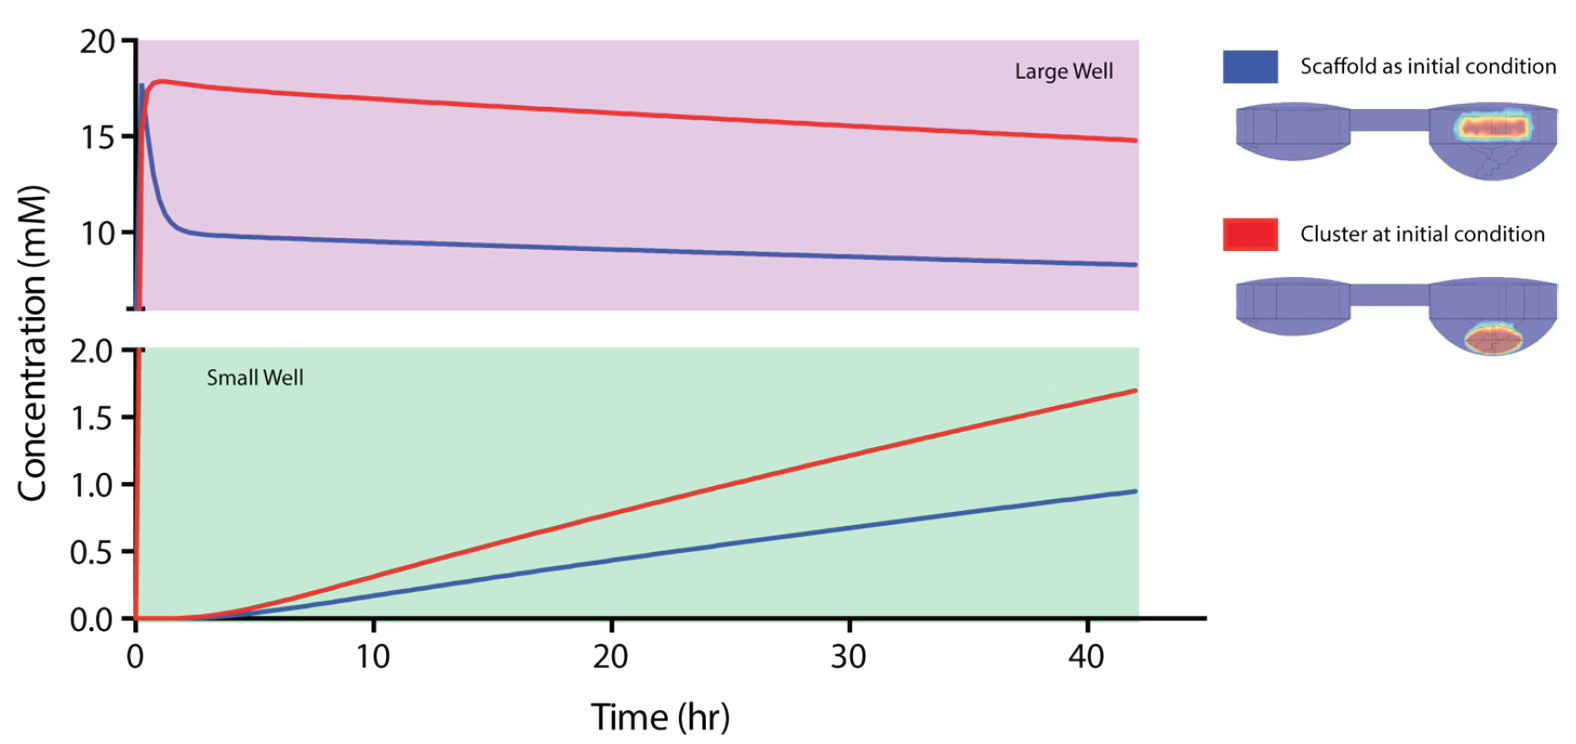
\includegraphics[width=4.5in]{/FigS3.png}
\caption{The average concentration in the bottom meniscus of each well following solute release in a modeled bone-like scaffold or cluster in the culture well.}
\label{figure:FigS3}
\end{figure}
% \chapter{Droplet Geometry}
\label{App:DropletGeometry}

There are many different ways to formulate the geometry of passive pumping between an input drop and an output drop. The aim of this appendix is to describe the droplet geometry in as many ways as possible so that it does not need to be significantly re-derived in the future. The following variables are used.

\begin{table}[htdp]
\caption{\textbf{Droplet geometry variable names and definitions}. The subscript $i$ denotes the number of the droplet/port/wetted area of interest.}
\centering
\begin{tabular}{ll}\toprule
Variable&Description\cr
\midrule
$a_{i}$&Radius of the port/wetted area\cr
$R_{i}$&Radius of curvature of the droplet\cr
$\R_{i}$&$R_{i}/a_{i}$ (dimensionless)\cr
$H_{i}$&Height of the droplet\cr
$\h_{i}$&$H_{i}/a_{i}$ (dimensionless)\cr
$C_{i}$&Vertical position of the center of the radius of curvature of the droplet\cr
$\C_{i}$&$C_{i}/a_{i}$ (dimensionless)\cr
$V_{i,hemi}$&$\frac{2}{3}\pi a_{i}^{3}$\cr
$V_{i}$&Volume of the droplet\cr
$\V_{i}$&$V_{i}/V_{i,hemi}$ (dimensionless)\cr
$\theta_{i}$&Contact angle of the droplet with the device\cr

\bottomrule
\end{tabular}
\end{table}%

First we define relationships between the various variables of interest.

\section{\texorpdfstring{Radius of Curvature, $R_{i}$ and $\R_{i}$}{Radius of Curvature, Ri and Ri}}%%%%%%%%%%%%%%

\begin{equation}
%\centering
\R_{i}=\frac{R_{i}}{a_{i}}
\end{equation}

\begin{equation}
%\centering
\R_{i}=\sin^{-1}(\theta_{i})
\end{equation}

\begin{equation}
%\centering
\R_{i}=\frac{\h_{i}^{2}+1}{2\h_{i}}
\end{equation}

\section{\texorpdfstring{Height, $H_{i}$ and $\h_{i}$}{Height, Hi and Hi}}%%%%%%%%%%%%%%%%%%%%

\begin{equation}
%\centering
\h_{i}=\frac{H_{i}}{a_{i}}
\end{equation}

\begin{equation}
%\centering
\h_{i}=\frac{1-cos(\theta_{i})}{sin(\theta_{i})}=tan\left(\frac{\theta_{i}}{2}\right)
\end{equation}

\begin{equation}
%\centering
\footnote{always produces result between 0 and $a$}\:
\h_{i}=\R_{i}\left(1-\sqrt{1-\frac{1}{\R_{i}^{2}}}\right)
\end{equation}

\begin{equation}
%\centering
\h_{i}=\left(\frac{1-\left(-2\V_{i}+\sqrt{1+4\V_{i}^{2}}\right)^{2/3}}{\left(-2\V_{i}+\sqrt{1+4\V_{i}^{2}}\right)^{1/3}}\right)
\end{equation}

\section{\texorpdfstring{Contact Angle, $\theta_{i}$}{Contact Angle, theta}}%%%%%%%%%%%%%%%%%%%%

\begin{equation}
%\centering
\footnote{always produces result between 0\Deg and 90\Deg}\:
\theta_{i}=\arcsin\left(\frac{1}{\R_{i}}\right)
\end{equation}

\begin{equation}
%\centering
\theta_{i}=2\arctan\left(\h_{i}\right)
\end{equation}

\begin{equation}
%\centering
\theta_{i}=2\arctan\left(\frac{1-\left(-2\V_{i}+\sqrt{1+4\V_{i}^{2}}\right)^{2/3}}{\left(-2\V_{i}+\sqrt{1+4\V_{i}^{2}}\right)^{1/3}}\right)
\end{equation}

\section{\texorpdfstring{Volume, $V_{i}$ and $\V_{i}$}{Volume, Vi and Vi}}%%%%%%%%%%%%%%%%%%%

\begin{equation}
%\centering
\V_{i}=\frac{V_{i}}{V_{i,hemi}}
\end{equation}

\begin{equation}
%\centering
\V_{i}=\frac{1}{4}\h_{i}(3+\h_{i}^2)
\end{equation}

\footnote{always results in a normalized volume between 0 and 1 (\ie , $0\le V\le V_{hemi}$ or $0$\Deg$\le\theta\le90$\Deg)\label{fn:Vol}}
\begin{equation}
%\centering
\V_{i}=\frac{1}{4}\R_{i}\left(1-\sqrt{1-\frac{1}{\R_{i}^{2}}}\right)\left(3+\R_{i}^{2}\left(1-\sqrt{1-\frac{1}{\R_{i}^{2}}}\right)^{2}\right)
\label{equ:VofR1}
\end{equation}

\footnote{always results in a normalized volume $> 1$ (\ie , $V_{i,hemi}\le V_{i}\le\infty$ or $90$\Deg$\le\theta_{i}\le180$\Deg)}
\begin{equation}
%\centering
\V_{i}=2\R_{i}^3 - \frac{1}{4}\R_{i}\left(1-\sqrt{1-\frac{1}{\R_{i}^{2}}}\right)\left(3+\R_{i}^{2}\left(1-\sqrt{1-\frac{1}{\R_{i}^{2}}}\right)^{2}\right)
\label{equ:VofR2}
\end{equation}

$^{\ref{fn:Vol}}$
\begin{equation}
%\centering
\V_{i}=\frac{V_{i}}{V_{i,hemi}}=\frac{1}{4}\tan\left(\frac{\arcsin\left(\frac{a_{i}}{R_{i}}\right)}{2}\right)\left(3+{\tan\left(\frac{\arcsin\left(\frac{a_{i}}{R_{i}}\right)}{2}\right)}^{2}\right)
\label{equ:VofR3}
\end{equation}

$^{\ref{fn:Vol}}$
\begin{equation}
%\centering
\V_{i}=\frac{1}{4}\tan\left(\frac{\theta_{i}}{2}\right)\left(3+{\tan\left(\frac{\theta_{i}}{2}\right)}^{2}\right)
\end{equation}

\begin{figure}[!ht]
\centering
\includegraphics[width=3.2in]{Theta.pdf}
\caption{\textbf{Dimensionless variable relationships in passive pumping}. Plot of $a/R$ and contact angle, $\theta$, with respect to normalized droplet volume, $\V$ (or $V_{i}/V_{i,hemi}$). Theta is measured at the contact point between the spherical drop and the horizontal surface extending toward the center of the port.}
\end{figure}

\section{\texorpdfstring{Location of Center of Radius of Curvature, $C_{i}$ and $\C_{i}$}{Location of Center of Radius of Curvature, Ci and Ci}}

\begin{equation}
%\centering
\C_{i}=\frac{C_{i}}{a_{i}}
\end{equation}

\begin{equation}
%\centering
\C_{i}=\h_{i}-\R_{i}
\end{equation}

\begin{equation}
%\centering
\C_{i}=-\R_{i}\sqrt{1-\frac{1}{\R_{i}^{2}}}
\end{equation}

\begin{equation}
%\centering
\C_{i}=-\R_{i}\cos\left(\theta_{i}\right)
\end{equation}



% \chapter{Diffusion Modeling}
\label{App:Diffusion}

\section{PDGF Modeling}
The PDGF signaling parameters are taken from an analysis performed by Lauffenburger \etal\ \cite{Lauffenburger:1989fy}. The threshold sensing concentration is based on the dissociation constant of PDGF given as, K$_{d}$ = 10$^{-10}$ - 10$^{-9}$ [mol/L]. The production rate, q$_{PDGF}$, is given as 10$^{-16}$ - 10$^{-15}$ [g/cell/min] which was cited as being taken from Leof \etal\ \cite{LEOF:1986uq}, a study using human foreskin fibroblasts. The molecular weight was estimated to be 30 [kDa]. Using the molecular weight we can convert the units of q$_{PDGF}$ to yield 5e-16/(30000*60) = 2.78e-22 [mol/cell/s]. The Einstein-Stokes equation gives $D$ = 79 [\textmu m$^{2}$/s] for the 30 [kDa] molecule.

\section{EGF Modeling}
EGF modeling was taken from work by Knauer \etal \cite{KNAUER:1984fj} and Starbuck \etal \cite{STARBUCK:1992kl}. This work is based on data obtained using human and mouse fibroblasts. The EGF complex internalization rate constant, k$_{eC}$, was measured to be  5.3e-3 [s$^{-1}$]. Half maximal response occurs at 0.15 [ng/mL] and 2000 surface complexes per cell. This means an internalization rate of 2000*5.3e-3 = 10.6 [molecules/cell/s]. The molecular weight of EGF and the EGF\slash EGF binding protein complex were cited as 6.4 and 74 [kDa] respectively. Converting units we get a 10.6/6.022e23 = 1.76e-23 [mol/cell/s] EGF uptake rate for fibroblast cells. Thus, $q_{max}$ = 2*1.76e-23 = 3.52e-23 [mol/cell/s]. Cellular affinity for EGF is about 4.69e-11 [mol/L] vs. a K$_{d}$ of 4.7e-9 [mol/L]. Again, using the Einstein-Stokes equation, a 6.4 [kDa] molecule gives a diffusion coefficient of D = 131 [\textmu m$^{2}$/s] and 58 [\textmu m$^{2}$/s] for a 74 [kDa] molecule. The latter is used to estimate the diffusing protein.

Factor uptake, q, is assumed to follow the Michaelis-Menten kinetics with respect to the concentration of a rate limiting factor (Eq \ref{App:Diffusion:equ:uptakeRate}). The value $q_{max}$ represents the maximum uptake rate per cell. $C_{cb}$ is the concentration of factor at the cell boundary and $C_{th}$ is the Monod or Michaelis-Menten constant. Per the definition of the Michaelis-Menten constant (Eq \ref{App:Diffusion:equ:uptakeRate}), when $C_{cb} = C_{th}$ then $q = q_{max}/2$. Thus, we use the threshold sensing concentration for the Michaelis-Menten constant. Therefore, when concentration at the cell boundary is 0, there is no uptake of factor, while at $C_{th}$, uptake is $q_{max}/2$.

\begin{equation}
\label{App:Diffusion:equ:uptakeRate}
q = \frac{q_{max}C_{cb}} {C_{th}+C_{cb}} = \frac{q_{max}} {1+\frac{C_{th}}{C_{cb}}}
\end{equation}

%\section{Basic geometries}
%\begin{figure}[!t]
%\centering
%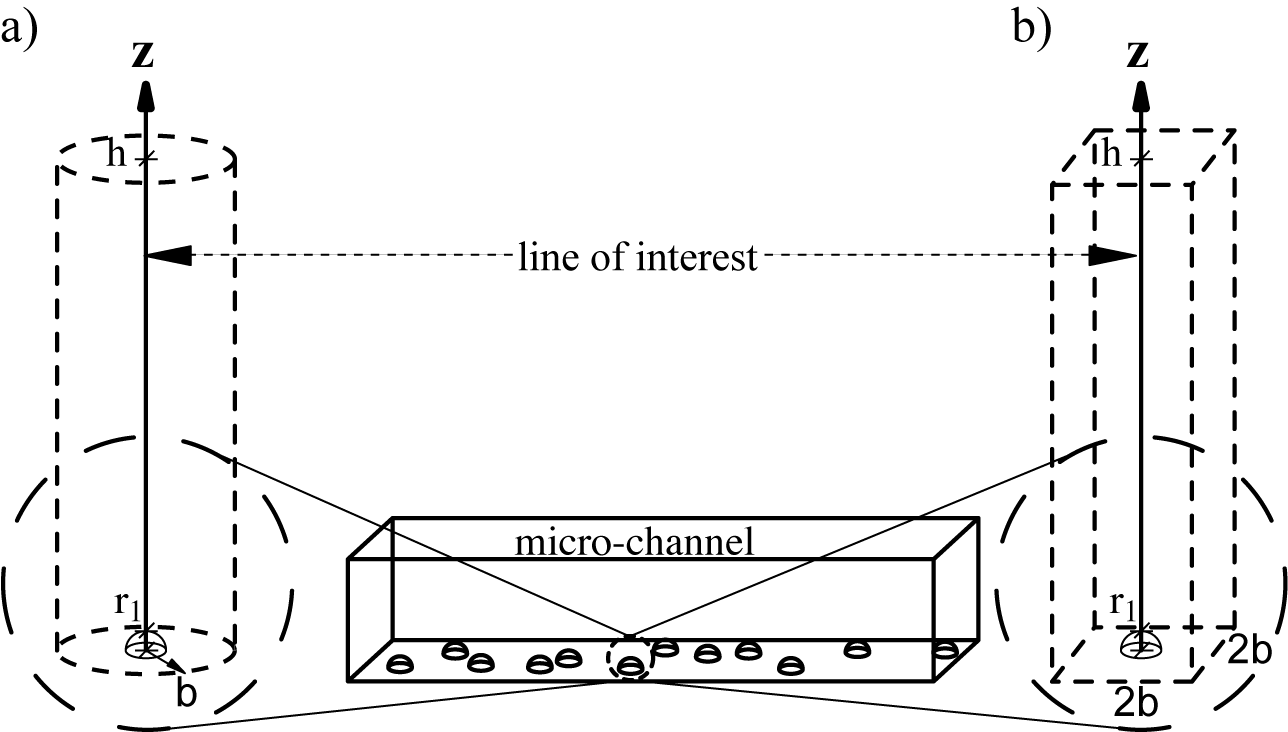
\includegraphics[width=3.5in]{Average_Geometries.pdf}
%\caption{Schematic representation of the cylindrical and rectangular geometry used to estimate the case of a single cell in culture with neighbors on a 2-D substrate. The area of the base of the unit-cylinder and unit-rectangle is equal to the area-per-cell on the substrate of the channel.}
%\label{App:Diffusion:diffusionGeom}
%\end{figure} 
%
%The line of interest labeled in Fig \ref{App:Diffusion:diffusionGeom} is the line on which a solution for the concentration will be approximated. The various ratios of the base dimension ($b$) to the height ($h$) and cell radius ($r_{1}$) will be accounted for in the boundary conditions of the one-dimensional approximation. The base dimension of the average volume is calculated from the average area per cell and the geometry. The cell is pictured as a hemisphere of radius $r_{1}$.  Items of interest emitted from or absorbed by the cell could include viruses, growth factors, cytokines, waste, or gas and have a wide range of diffusivities. The local environment of the cell has zero flux on all the walls where, on average, adjacent cells are assumed to be producing the same molecule at approximately the same rate.  An arbitrary boundary condition can be imposed at the top of the channel, $z=h$. However, we are restricted to a zero flux boundary condition at the bottom surrounding the cell, $z=0$.
%
%\section{Approximation Method}
%FE models of the average volume show that there appear to be two important regions of the model. The spherically shaped region closest to the cell and the very linear region extending far from the cell along the line of interest. These observations suggest it might be possible to add the solution of a spherical system that only depends on the radius, $r$, with a one-dimensional solution in Cartesian coordinates to obtain a total solution with sufficient accuracy to model the average cellular microenvironment (see Fig \ref{App:Diffusion:boundaries}). The idea of a linear combination to obtain the approximation is shown in Eq \ref{equ:linAdd} where $\alpha$ and $\beta$ represent the weighting of the terms in the total solution. As an addition note, other methods other than a simple linear addition were investigated, such as those that would transition between the solutions or vary the weighting with distance along the line of interest, yet they produced only slightly better results with the disadvantage of added complexity. Subscript $a$ refers to the approximation obtained from the one-dimensional solutions. Subscript $s$ refers to the one-dimensional spherical system and $c$ refers to the one-dimensional Cartesian system.
%
%\begin{figure}[!ht]
%\centering
%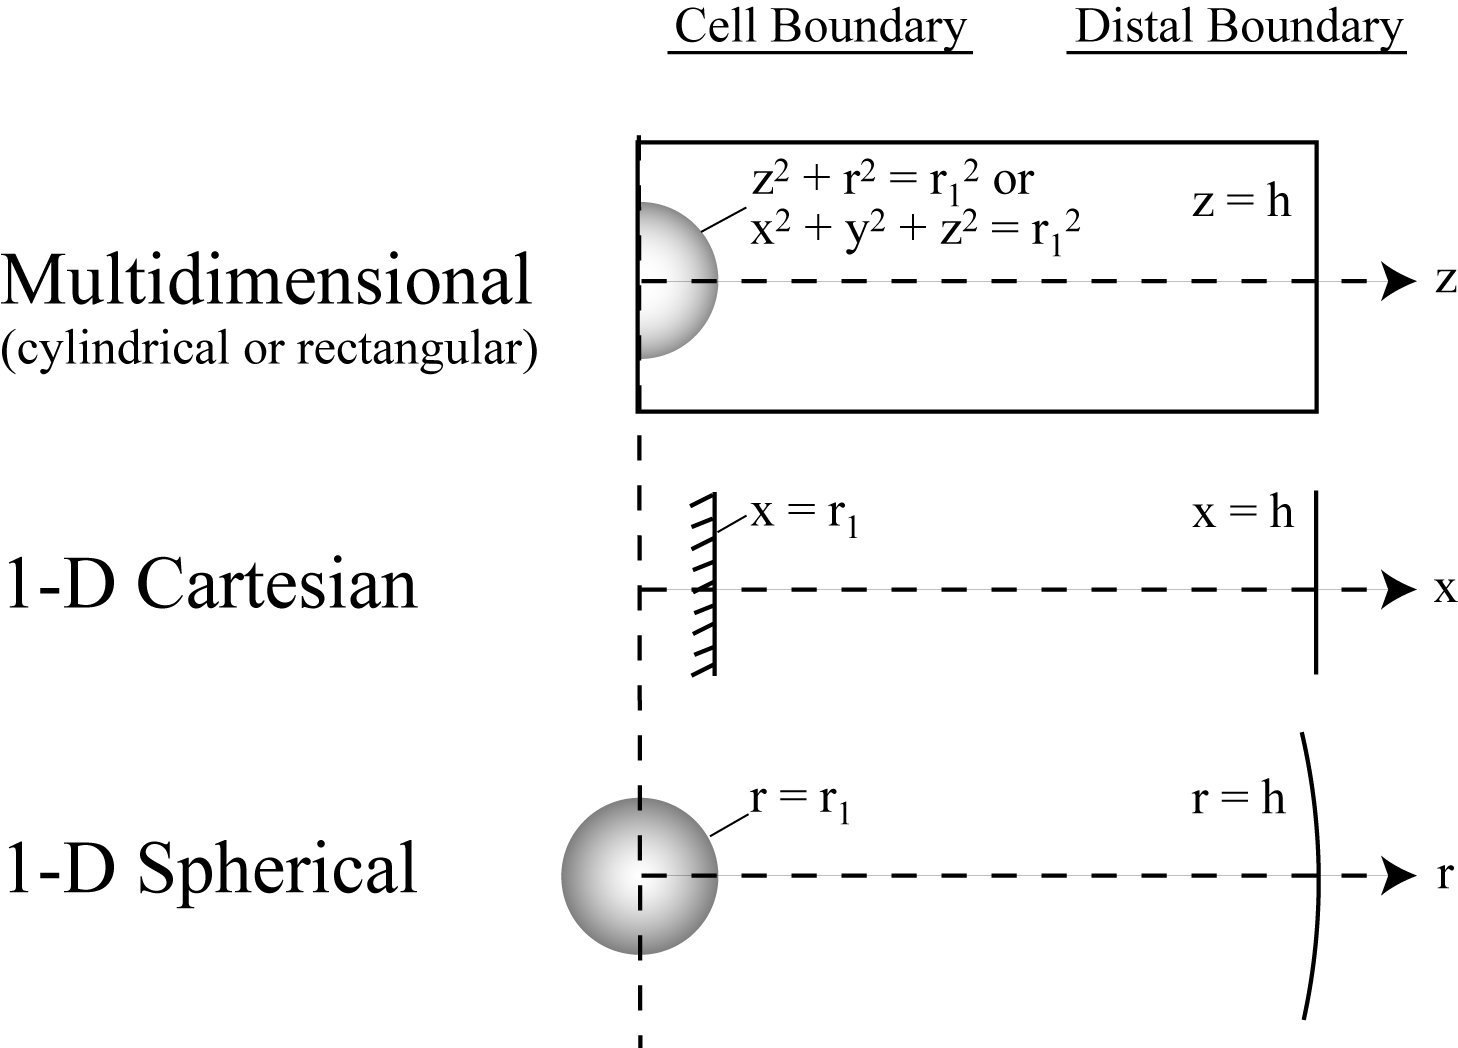
\includegraphics[width=3.5in]{Diffusion_Boundaries.pdf}
%\caption{Coordinate systems for the multidimensional models as well as the one-dimensional models.}
%\label{App:Diffusion:boundaries}
%\end{figure}
%
%
%\begin{equation}
%C_{a} = \alpha \, C_{s} + \beta \, C_{c}
%\label{equ:linAdd}
%\end{equation}
%
%Two conditions were imposed on the boundary conditions of the one-dimensional solutions to effectively determine $\alpha$ and $\beta$. The first condition was the conservation of mass. The change in average concentration with time for the volume must be the same between the multidimensional model and the approximation, as shown in Eq \ref{equ:balMass}. The second imposed condition is that the sum of the concentration gradients used in the one-dimensional system must equal the concentrations gradient perpendicular to cell boundary in the multidimensional model. The second condition is shown in Eq \ref{equ:balGrad} where $\overrightarrow{n}$ is the unit vector that points outward normal to the cell surface. Subscript $m$ refers to the multidimensional system in which all geometry is modeled precisely. 
%
%\begin{equation}
%\frac{d \overline{C}_{m}}{ d t} = \frac{ d \overline{C}_{s}}{ d t} + \frac{ d \overline{C}_{c}}{ d t}
%\label{equ:balMass}
%\end{equation}
%
%\begin{equation}
%\left( \frac{\partial C_{m}}{ \partial n} =  \frac{ \partial C_{s}}{ \partial r} + \frac{ \partial C_{c}}{ \partial x} \right) \Big |_{\textrm{\tiny cell boundary}}
%\label{equ:balGrad}
%\end{equation}
%
%By combining these conditions, the following equations for the flux boundary condition at a given time is as follows.
%
%\begin{equation}
%\label{equ:gradCart}
%\left(\frac{\partial{C_{c}}}{\partial{x}} = \frac{\partial C_{m}}{ \partial n}  \frac{ \mu-\eta}{\mu-\frac{1}{h-r_{1}}}\right) \Big |_{\textrm{\tiny cell boundary}}
%\end{equation}
%
%\begin{equation}
%\label{equ:mu}
%\mu=\frac{-3r_{1}^{2}}{h^{3}-r_{1}^{3}}
%\textrm{, and}
%\end{equation}
%
%\begin{equation}
%\label{equ:eta}
%\eta=\frac{-2\pi r_{1}^{2}}{\pi b^{2}h-\frac{2}{3}\pi r_{1}^{3}} \textrm{   (cylindrical)}
%\end{equation}
%
%\begin{equation}
%\label{equ:eta}
%\eta=\frac{-2\pi r_{1}^{2}}{4b^{2}h-\frac{2}{3}\pi r_{1}^{3}} \textrm{   (rectangular)}
%\end{equation}
%
%Eq \ref{equ:balGrad} is then used to calculate the flux boundary condition $\partial C_{s}/ \partial r$ at the cell boundary from the solution to Eq \ref{equ:gradCart}. Eq \ref{equ:gradCart} is used to create Fig \ref{App:Diffusion:ratio} where the ratio of the boundary conditions is between 0 and 1. If the ratio is $<0$ or $>1$, then the approximation method breaks down producing opposing boundary conditions. For the cylindrical geometry the ratio is 0 when $h/b= 3/ \sqrt{6}$ and where $h/b=\sqrt{6/ \pi}$ in the case of the rectangular geometry. Similarly, the ratio is 1 when $b=r_{1}\sqrt {-6h( 2r_{1}-3h}/(3h)$ and $b=r_{1}\sqrt {-6h\pi( 2r_{1}-3h)}/(6h)$ for the cylindrical and rectangular case respectively. The ratio is used to solve the one-dimensional problems over the distance $r=r_{1}\,...\,h$ with a diffusion coefficient, $D$, for the molecule of interest.
%
%\begin{figure}[!ht]
%\centering
%\includegraphics[width=2.5in]{Ratio_080207.pdf}
%\caption{Plot of $(\partial C_{c}/ \partial x)/(\partial C_{m}/ \partial n)$ for various ratios of $b/r_{1}$ and $h/r_{1}$ for the cylindrical geometry shown in Fig Xa.}
%\label{App:Diffusion:ratio}
%\end{figure}
%
%
%\section{Results and Discussion}
%\subsection{Constant flux boundary condition}
%The FE modeling software, COMSOL (PLACE), is used in conjunction with Matlab to produce all the transient diffusion results. The accuracy of the approximation is examined first using the simple case of a constant flux boundary condition on the cell. A simulation is performed for a cell with an average cell with a diameter of 10 $\mu$m producing glucose with a diffusion coefficient $D$ = 0.0016 mm$^{2}$/s at a rate of $R$ = 5.56$\times$10$^{-6}$ nmol/cell/s in a microchannel of height $h$ = 250 $\mu$m with 300 cells/mm$^{2}$. 
%%
%%\begin{figure}[!ht]
%%\centering
%%\includegraphics[width=2.5in]{box.jpg}
%%\caption{Plot of concentration vs. time for the cell boundary and ceiling of the microchannel for the multidimensional model, $C_{m}$, and the approximation, $C_{a}$, for the geometry shown in Fig Xb and parameters listed above.}
%%\label{App:Diffusion:graphCt}
%%\end{figure}
%
%Fig \ref{App:Diffusion:graphCt} shows how the approximation tracks with the 3-D COMSOL model. Notice that the difference between the approximation and multidimensional model grows until it stabilizes to a constant difference when the system stabilizes and uniformly raises in concentration over time according to Eq \ref{equ:balMass}. In order to present a comparison of the multidimensional model and approximation over a large range of geometric aspect ratios, the system is made dimensionless. Time is made dimensionless using Eq \ref{equ:tau}. Error will be reported as the percent difference between the multidimensional model and the approximation calculated at the cell boundary for $\tau$ = 1. The value of 1 is chosen for $\tau$ as it is indicative of the time it takes for a system to approach steady-state with constant flux boundary conditions. Error is plotted for various aspect ratios of the cylindrical geometry on a contour plot in Fig \ref{App:Diffusion:errorCyl}. The same is done for the rectangular geometry in Fig \ref{App:Diffusion:errorRect}.
%
%\begin{equation}
%\label{equ:tau}
%\tau = \frac{ \left( h - r_{1} \right) ^{2}}{2D}
%\end{equation}
%
%\begin{figure}[!ht]
%\centering
%\includegraphics[width=2.5in]{Cylindrical_080207.pdf}
%\caption{Error results for a constant flux boundary condition. Above is a plot of $100 \% \times (C_{m}-C_{a})/C_{m}$ for various ratios of $b/r_{1}$ and $h/r_{1}$ for the cylindrical geometry shown in Fig Xa.}
%\label{App:Diffusion:errorCyl}
%\end{figure}
%
%\begin{figure}[!ht]
%\centering
%\includegraphics[width=2.5in]{/Users/warrick/Documents/Videos_and_Images/box.jpg}
%\caption{Error results for a constant flux boundary condition. Above is a plot of $100 \% \times (C_{m}-C_{a})/C_{m}$ for various ratios of $b/r_{1}$ and $h/r_{1}$ for the rectangular geometry shown in Fig Xb.}
%\label{App:Diffusion:errorRect}
%\end{figure}
%
%Results from this section suggest that the method of approximation is valid and quite accurate for a large range of aspect ratios and cell densities. Figs \ref{App:Diffusion:errorCyl} and \ref{App:Diffusion:errorRect} indicate errors typically less than 10\% in magnitude within the applicable range of aspect ratios shown in Fig \ref{App:Diffusion:ratio}. Typical microchannel heights for cell culture are many multiples of the cell radius. If a cell is roughly 10 $\mu$m in diameter, and $h/r=30$, the microchannel height is approximately 150 $\mu$m and the approximation would be appropriate where cell density is $>57$ cells/mm$^{2}$. If $h/r=50$, then the channel height would be 250 $\mu$m and the approximation would be appropriate for cell densities $>20$ cells/mm$^{2}$. Thus, the approximation is valid for many typical cell culture parameters and can be applied as the cells proliferate and approach confluency.
%
%
%\subsection{Transient flux boundary condition}
%With positive results in the case of constant flux it is now necessary to address the situation of transient flux. The flux boundary condition is made to follow a Gaussian profile over time. A Gaussian profile is determined by the value for the mean ($\bar x$), standard deviation ($\sigma$), and maximum ($y_{max}$). The profile mean is at $\tau=1.\bar3$. $\sigma$ corresponds to $0.\bar3$ units of dimensionless time, $\tau$. Thus, at $\tau=0$ the flux is at $-4\sigma$ along the Gaussian profile. This situation might approximate the transient response of a cell to a stimulus. Typical results for the two methods using a cylindrical geometry are plotted in Fig \ref{App:Diffusion:errorTime} along with a normalized plot of the flux profile. The difference between the two methods increases during the rise in concentration and then approaches zero as the system stabalizes. The percent difference in cell boundary concentration at the peak of the flux (i.e. at $\tau=1.\bar3$) between the multidimensional model and the approximation using the cylindrical geometry is reported in Fig \ref{App:Diffusion:errorTime} for various aspect ratio as a contour plot. Results show good agreement with the multidimensional model again with similar errors as the case of a constant flux boundary condition.
%
%\begin{figure}[!ht]
%\centering
%\includegraphics[width=2.5in]{Cylindrical_Transient_080207.pdf}
%\caption{Error results for a transient flux boundary condition following a Gaussian profile. Above is a plot of $100 \% \times (C_{m}-C_{a})/C_{m}$ for various ratios of $b/r_{1}$ and $h/r_{1}$ for the cylindrical geometry shown in Fig Xa.}
%\label{App:Diffusion:errorTime}
%\end{figure}
%
%
%
%
%
%
%
%
%\subsection{Dynamics of diffusion and biology}
%One typical change during \textit{in-vitro} cell culture is the cell number. A major advantage of reducing the multidimensional diffusion problem to a one-dimensional problem is that changes in cell number (i.e. the spacing parameter $b$) can be accounted for using Eq \ref{equ:gradCart}. Thus, the approximation method can accommodate changes in cell density due to cell proliferation, death, or apoptosis by adjusting the flux boundary condition accordingly. There is no need to interrupt the model and incrementally re-mesh the geometry making the FE model impractical for many users. 
%
%Through simulation one can also identify when diffusion dynamics result in significant concentration differences within the system and could possibly affect cell behavior. One way to estimate the concentration distribution within the channel is to look at a steady-state system with constant flux at the cell. At steady-state, the difference, $\triangle C$, between the concentration at the cell boundary and at the ceiling of the channel for the approximation are given by the following equations.
%
%\begin{equation}
%\label{equ:steady}
%\triangle C=\frac{\alpha}{r_{1}-h}+\frac{\beta}{2}(r_{1}^{2}-h^{2}) + \frac{h-r_{1}}{2} \left(\frac{\partial C_{c}}{\partial x} \big |_{x=r_{1}}\right)
%\end{equation}
%
%\begin{equation}
%\label{equ:alpha_2}
%\alpha = -\beta r_{1}^{3}+ r_{1}^{2} \left(\frac{\partial C_{s}}{\partial r} \big |_{r=r_{1}}\right)
%\end{equation}
%
%\begin{equation}
%\label{equ:beta_2}
%\beta = -\frac{r_{1}^{2}}{h^{3}-r_{1}^{3}} \left(\frac{\partial C_{s}}{\partial r} \big |_{r=r_{1}}\right)
%\end{equation}
%
%$\triangle C$ is affected by the dimensions of the system and the rates of influx and efflux to and from the cell. Concentration differences increase with increasing dimensions and increasing rates of flux. $\triangle C$ can be compared to other important concentration parameters of the system. For example, if the initial concentration of nutrients within a microchannel, $C_{0}$ is $\gg \triangle C$ then the dynamics of diffusion will have little relative effect on concentrations. However, if $C_{0} \sim \triangle C$ or if nutrients are depleted to a point where the average concentration, $\overline{C}$, is on the order of $\triangle C$, then the dynamics of diffusion could play an important role in system behavior. Another consideration is the relative size of $\triangle C$ to threshold concentrations of the cell, $C_{t\_i}$. If $\triangle C \ll C_{t\_i}$, then diffusion dynamics will play little role in affecting concentrations near thresholds.
%
%The time scale and biological dynamics of the system can also be important when considering the role of diffusional effects. For example, if the time scale of the biological process is on the order of $\tau$, an estimate of the time it takes for diffusion to redistribute the soluble factor (see Eq \ref{equ:tau}), the dynamics of the biological process and diffusion will interact for unique system behavior. Alternatively, even if $\triangle C$ is relatively small and $\tau$ is much less that the time scale of the biological process, effects of the concentration distribution could be significant when integrated over a large time. For example, if a soluble factor played a critical role in exponential cell growth, over time, the effects of a small difference in concentration could be greatly magnified over time. Similarly, biological processes with tight thresholds or feedback loops could be very sensitive to subtle changes in microenvironmental concentrations due to diffusional dynamics.
%
%Some of the considerations that were just discussed can be seen in a simple model of cell growth in response to a rate limiting factor. Factor concentration and cell proliferation are dynamically modeled together using Matlab and a Crank-Nicolson method for modeling diffusion.
%
%Proliferation rate is assumed to follow the Michaelis-Menten kinetics with respect to the concentration of a rate limiting factor (Eq \ref{equ:prolRate}). $u_{max}$ represents the maximum proliferation rate of the cells. $C$ is the concentration of factor at the cell boundary and $K_{m}$ is the Monod or Michaelis-Menten constant, which is the concentration at which the proliferation is at $u_{max}/2$. Population kinetics are then modeled using Eq \ref{equ:pop} where N is the cell number. Many other terms could be included into Eq \ref{equ:prolRate} to more accurately model the system such as the possible negative effects of waste concentration or cell contact inhibition. As more soluble factors are added to the system, a separate, simultaneous model of diffusion is needed to keep track of each concentration. In the interest of simplicity, extra terms are neglected in this example. The result of the simulation (the dynamic model) will be compared to a model that assumes even and constant mixing of the microchannel (the evenly-mixed model). The hypothesis is that the distribution of soluble factors can play a significant role in the dynamics of the system as a whole.
%
%\begin{equation}
%\label{equ:prolRate}
%u = \frac{u_{max}C} {K_{m}+C}
%\end{equation}
%
%\begin{equation}
%\label{equ:pop}
%u = \frac{1}{N} \frac{dN}{dt}
%\end{equation}
%
%The cell number over time is plotted for the dynamic and evenly-mixed model are plotted over time to show the difference in the results. Tab X shows simulation results for a wide variety of parameters. In some cases, there is enough factor to double the population size while in other cases, the  factor is depleted and growth rate approaches $0$. If the population doubles, the time at which it doubles is reported as $t_{2N_{0}}$. If the population growth rate falls to one tenth of the maximum growth rate, the cell number and time, $t_{u_{max}/10}$, at which it occurs are recorded. The ratio  $(\partial C_{c}/ \partial x)/(\partial C_{m}/ \partial n$) is always between 0 and 1 in the simulations. Also $b/r$ is always $>1$. Corresponding values of $\triangle C$ and $\tau$ are given for later analysis and discussion. The time scale of the biological process is estimated here as the doubling time of the cell population when the proliferation rate is at a maximum and is referred to using $t_{bp}$.
% \chapter{Concentrator: Additional Information}
\label{App:Concentrator}

\section{Estimation of Cell Number Limit}

A lower limit of ~50,000 cells is calculated based on a seeding density of 250 cells/mm$^{2}$ for culture in a microchannel with a height of 250 \textmu m (\ie , a density of 1000 cells/\textmu L). It is also assumed that the original sample is centrifuged to a minimum volume of 50 \textmu L to avoid aspiration of any concentrated cells. The limit is specific to the application.

\section{Initial Design Approach for Concentrator Design}

The dimensions of the initial device design were chosen in order to produce a shear stress of roughly 0.1 dynes/cm$^{2}$ within the collection region and to give the cells a chance to settle to the substrate after entry into the collection region (i.e., t$_{set}/t_{res}$ $\approx$ 1). Transport channel dimensions were then varied to produce shear rates and residence times above and below these thresholds to explore the appropriate conditions for proper cell retention. Channel resistances were estimated using the Washburn Law and applied to an electrical circuit analog for fluid flow. Passive pumping pressures were estimated using Eq \ref{equ:laplace}.

Design II differs from Design I primarily in the dimensions of the collection region. The width was increased while the height was reduced based on the dimensional analysis described in the main text. Channel height does not affect t$_{set}/t_{res}$ but can affect shear. When channel width increases, t$_{set}/t_{res}$ decreases, thereby increasing the chance for cell capture. Thus Design II was viewed as an improvement to Design I.

\section{Cell Loss Modeling}

COMSOL Multiphyisics v3.4 (Burlington, MA) was used to obtain steady state solutions for fluid flow through Deisgn I and II. First a simulation of the whole device (using symmetry) was used to determine that the pressure drops across the transport channels (from center input to the outer ring) were within 0.55\% of one another (see Fig \ref{fig:evenPressure}). Because flow through each transport is nearly identical, the 3D model was simplified to include only one of the repeating sections of the collection region. This repeating section was then divided in half along its line of symmetry. This allowed a finer meshing of the region for more detailed analysis.

\begin{figure}[!b]
\centering
\includegraphics[width=3in]{EvenPressure_Composite.pdf}
\caption{\textbf{Plot of normalized pressure along device axis of symmetry}. The pressure at the input is defined as 1 whereas the pressure nearest the output port is defined as zero. The normalized pressure farthest from the output, at the intersection of the transport channel and outer ring, is then 0.0055.}
\label{fig:evenPressure}
\end{figure}

A threshold of 0.1 dynes/cm$^{2}$ was used to help determine cell loss (see Fig \ref{fig:shearStress}). If streamline calculations suggest that a cell settles to the surface before reaching the collection region exit, then the shear stress is calculated at that location. If the shear stress at that location is below the threshold of 0.1 dynes/cm$^{2}$, then the cells that follow that streamline are assumed to be captured. If the shear stress is too high, it is assumed the cells are lost. Only one half of the region depicted was simulated using a symmetry boundary condition along the center line. The results are reflected to better indicate the shape of the repeating portion of the collection region.

\begin{figure}[!b]
\centering
\includegraphics[width=3in]{ShearStress.pdf}
\caption{\textbf{Concentrator shear stress near the substrate}. Shear stress one cell radius (6.25 \textmu m) above the substrate for a total device flow rate of 5 \textmu L/min. The color legend indicates shear stresses between 0 and 0.1 dynes/cm$^{2}$. Simulations assume that cells are not collected in regions with a shear stress above 0.1 dynes/cm$^{2}$ (white areas near inlet and outlet). Flow velocities in the x-direction half way through the collection region are shown as a slice heat map.}
\label{fig:shearStress}
\end{figure}

Streamlines were modeled by assuming that the cell settles at a rate of 2.7 \textmu m/s, a value obtained using the Stokes drag of the particle. Streamlines were calculated using COMSOL starting at the entrance into the collection region (see Fig \ref{fig:streamlines}). The starting points form a grid in the entrance. The size of the cell prohibits the center of the cells from following streamlines that are less than a radius from the transport channel wall. Thus the grid of streamline start-points begin one radius in from the transport channel walls. The streamlines are followed until the ``cell'' exits the modeled space (\ie , the substrate or collection region exit).

\begin{figure}[!t]
\centering
\includegraphics[width=3in]{StreamlinePlot.pdf}
\caption{\textbf{Particle streamlines within the concentrator}. Example plot of streamlines used to calculate percent loss for a given flow condition and device design. Streamlines begin from a grid of locations at the entrance to the collection region. The streamlines are followed until they exit the collection region or intersect with the substrate of the device. These streamlines are calculated assuming the cell settles at a velocity of 2.7 \textmu m/s and used in further calculations to determine if the cell is captured or lost. A high density of streamlines is used to increase the precision of the simulated loss measurements.}
\label{fig:streamlines}
\end{figure}

By numerically integrating the inverse of the particle velocity along the length of a streamline, one can obtain the time it takes for the particle to reach a location along that streamline. The amount of fluid that has flowed along the streamline is equal to the flow rate at the starting point times the time that has been allowed to pass. The flow rate at the starting point of the streamline is dictated by the fluid velocity and the grid spacing for the streamlines. The information regarding the time for the particles to reach a location along the streamline can be converted to volume information using this flow rate. In other words, the data is transformed such that it represents how much volume must flow into the device to move the particles to a certain position along a streamline. The volume-position data for each streamline is then used to determine how many cells would be lost for a given streamline, cell suspension density, and volume that has been pumped at a predetermined average flow rate. This method simplifies pumping as a square wave instead of a natural passive pumping flow profile. The average flow rate used to calculate cell loss is determined by taking the volume-averaged flow rate of a passive pumping profile that matches the given experimental condition. The method described here does take into account fixed-volume effects as described in the main article. If not enough fluid has been put through the device to cause any cells to leave the collection region on a streamline, all the cells on that streamline are considered captured.

\section{Experimental Calculation of \texorpdfstring{{\boldmath$t_{set}/t_{res}$}}{tset tres}}

Passive pumping is a dynamic phenomena where pressure changes with the geometry of the droplet that drives fluid flow. In order to estimate a value for $Q$ from this dynamic process for use in Eq \ref{equ:ratio}, an `average' value must be chosen.  A volume-averaged flow rate is chosen instead of a time-averaged flow rate as we are interested in the average velocity that a particular unit volume sees within the collection region. The volume-averaged flow rate can be calculated from the volume-averaged pressure, $P$, and resistance, $Z$, given that $P=QZ$ for low Reynolds number flow. The volume-averaged pressure can be determined using the relationship between droplet geometry and pressure given by the Young-Laplace equation (Eq \ref{equ:laplace}). The resistance of the device was determined using experimental measurements of passive pumping times and droplet geometries, as measured using a goniometer. The data was matched with an analytical solution for passive pumping\cite{Berthier:2007mi} to determine the device resistance, $Z$, needed to produce the appropriate pumping time given the initial droplet geometry. This resistance, volume-averaged pressure, and device geometry ($A$) are then used to calculate an appropriate flow velocity, $v_{f}$, for estimating $t_{set}/t_{res}$. The cross sectional area, A, is calculated at the average radius of the device collection region, $r_{d}$ = 3.75 mm. 

Calculations of flow rate in Design II are summarized in Fig \ref{fig:pp}. Instead of plotting pressure \vs\ volume, device geometry and resistance are taken into account to plot flow rate \vs\ volume. Results for a 6 \textmu L and 15 \textmu L drop are shown as these are the two different sizes of drops used experimentally. Simulated cell trajectories are depicted in a cross-section view of the collection region and show how higher flow rates cause more cell streamlines to flow out of the collection region instead of reaching the substrate. The trajectories are simulated using steady-state conditions and are only shown for those along the centerline of the transport channels.

% \chapter{Oscillatory Flow}
\label{App:Oscillator}

Below is a table with the constants and variables used throughout this appendix with their definitions.

\begin{table}[!ht]
\caption{\textbf{Variables and constants of fluid flow and their definitions}.}
\centering
\begin{tabular}{cp{10.5cm}}\toprule
Variable/Constant & Description \cr \midrule
$p$ & pressure \cr
$\delta$ & constant pressure gradient amplitude \cr
$\delta_{o}$ & oscillating pressure gradient amplitude \cr
$\rho$ & fluid density \cr
$\mu$ & dynamic viscosity of the newtonian fluid \cr 
$\nu$ & kinematic viscosity, $=\mu/\rho$ \cr
$f$ & frequency of the oscillatory pressure gradient \cr
$\omega$ & radial frequency, $=2\pi f$ \cr 
$h$ & the full height of the channel \cr
$\lambda$ & penetration depth, $=\sqrt{2\nu/\omega}$ \cr 
$u$ & fluid velocity \cr
$\bar u$ & average fluid velocity \cr
$u_{max}$ & maximum fluid velocity \cr
$\tau_{wall}$ & fluid shear stress at the top and bottom surface of the channel \cr
$\tau_{wall, o}$ & fluid shear stress at the top and bottom surface of the channel due to the oscillatory component of flow\cr
$\gamma_{wall}$ & fluid shear rate at the top and bottom surface of the channel \cr
\bottomrule
\end{tabular}
\label{tab:}
\end{table}

We first present the solution to steady laminar flow between parallel plates as it will be references later in the context of oscillatory flow.

\section{Steady Laminar Flow Between Parallel Plates}
With the origin positioned half way between the plates (\ie , $y=0$) and the full height of the channel defined as $h$, the equation for $u$, the velocity in the x-direction is as follows.

\begin{equation}
\centering
u= \frac{1}{2\mu}\left[\frac{d}{dx}(p+\rho g z)\right]\left(\left(y-\frac{h}{2}\right)^{2}-\frac{h^{2}}{4}\right)
\label{equ:u}
\end{equation}
The flow rate through the cross section, where $b$ is the width that is $\gg h$ is as follows.
\begin{equation}
\centering
Q=-\frac{bh^{3}}{12\mu}\left[\frac{d}{dx}(p+\rho g z)\right]
\label{equ:Q}
\end{equation}
The average velocity of fluid between the plates is
\begin{equation}
\centering
\bar u = -\frac{h^{2}}{12\mu}\left[\frac{d}{dx}(p+\rho g z)\right] = \frac{Q}{bh} = \frac{2}{3}u_{max}.
\label{equ:ubar}
\end{equation}
The wall shear stress is given by the following.
\begin{equation}
\centering
\tau_{wall} = -\frac{h}{2} \left[\frac{d}{dx}(p+\rho g z)\right] = \frac{6\mu Q}{bh^{2}} = 2\mu \gamma_{wall}
\label{equ:tauWall}
\end{equation}

\section{Oscillatory, Non-Turbulent Flow Between Parallel Plates}

The mathematical analysis of oscillatory flow in a microchannel that can be approximated as a parallel plate flow chamber is presented here along with analysis of how much the surface tension at the ports of a tubeless microchannel influences flow. The following closed form solutions for oscillatory flow are reproduced from Bacabac \etal, 2005 \cite{Bacabac:2005ax} who compiled the information from Landau \etal, 1959 \cite{Landau:1959vh}. 

The equation for the velocity $u$ at vertical position $y$ in the channel at time $t$ where $y=0$ is half-way between the plates and h is the distance between the plates is given by Eq \ref{equ:uofyt} with subelements given by the equations that follow.

\begin{equation}
u(y,t)=C_{1}(y)+C_{2}(y)cos(\omega t)+C_{3}(y)sin(\omega t)
\label{equ:uofyt}
\end{equation}

\begin{equation}
C_{1}(y)=-\frac{\delta}{2\mu}\left(y^{2}-\frac{h^{2}}{4}\right)
\label{equ:C1}
\end{equation}

\begin{equation}
C_{2}(y)=\frac{\delta_{0}}{\rho\omega}\left[\frac{CC\left(\frac{-y+\frac{h}{2}}{\lambda},\frac{y+\frac{h}{2}}{\lambda}\right)+CC\left(\frac{y+\frac{h}{2}}{\lambda},\frac{-y+\frac{h}{2}}{\lambda}\right)}{cc_{+}\left(\frac{h}{\lambda}\right)}-1\right]
\label{equ:C2}
\end{equation}

\begin{equation}
\footnote{I believe that there is a typo in this equation of Bacabac \etal . The discrepancy is in the signs of the arguments of the second SS function. Otherwise, the results do not match the results in the paper or those obtained using COMSOL simulation as a secondary check.}C_{3}(y)=\frac{\delta_{0}}{\rho\omega}\left[\frac{SS\left(\frac{-y+\frac{h}{2}}{\lambda},\frac{y+\frac{h}{2}}{\lambda}\right)+SS\left(\frac{y+\frac{h}{2}}{\lambda},\frac{-y+\frac{h}{2}}{\lambda}\right)}{cc_{+}\left(\frac{h}{\lambda}\right)}\right] 
\label{equ:C3}
\end{equation}

\begin{equation}
\lambda = \sqrt{\frac{2\nu}{\omega}}
\label{equ:lambda}
\end{equation}


\begin{equation}
\begin{array}{r@{=}l}
SS(x_{1},x_{2})&\sin(x_{1})\sinh(x_{2}) \cr
CC(x_{1},x_{2})&\cos(x_{1})\cosh(x_{2}) \cr
ss_{\pm}(x)&\sin(x)\pm\sinh(x) \cr
cc_{\pm}(x)&\cos(x)\pm\cosh(x) \cr
\end{array}
\label{equ:C4}
\end{equation}

From these solutions, Bacabac \etal\ defined correction factors for the amplitude of the fluid flow rate and wall shear stress amplitude by normalizing results by the value predicted for static flow. Thus, when the correction factors are significantly different than 1, static solutions to the flow are no longer good approximations and dynamic effects are becoming significant. $T$ is the wall shear stress correction factor (when the flow rate is known) while $K$ is the correction factor for the amplitude of the flow rate, $q$ when the pressure gradient is known. Thus, if one is predicting shear when the pressure gradient is known, one must correct the flow rate using $K$ and plug the adjusted flow rate into the equation for shear which is then adjusted by $T$.

I was unable to successfully reproduce results given the Bacabac version of the equation for $K$ but was able to implement $T$ and the product $TK$, from which $K$ can be obtained through division. The following equations are used to predict flow and wall shear stress due to the oscillatory component of flow.

\begin{equation}
T(h/\lambda) = \frac{1}{3\sqrt{2}}  \frac{\frac{h}{\lambda}}{cc_{+}(\frac{h}{\lambda})}   \sqrt{\frac{(\sin(h/\lambda))^{2}+(\sinh(h/\lambda))^{2}}{1-\frac{2(\frac{\lambda}{h})ss_{+}(h/\lambda)}{cc_{+}(h/\lambda)}-\frac{2(\frac{\lambda}{h})^{2}cc_{-}(h/\lambda)}{cc_{+}(h/\lambda)}}}
\label{equ:T}
\end{equation}

\begin{equation}
T(h/\lambda)K(h/\lambda) = \frac{\sqrt{\left(ss_{-}(h/\lambda)\right)^{2}+\left(ss_{+}(h/\lambda)\right)^{2}}}{\frac{h}{\lambda}\;cc_{+}(h/\lambda)}
\label{equ:TK}
\end{equation}

\begin{equation}
q_{o}=\frac{bh^{3}\gamma_{o}}{12\mu}K(h/\lambda)
\label{equ:q}
\end{equation}

\begin{equation}
\tau_{wall, o}=\frac{6\mu q_{o}}{bh^{2}}T(h/\lambda)=\frac{h\gamma_{o}}{2}T(h/\lambda)K(h/\lambda)
\label{equ:tau}
\end{equation}

Bacabac \etal\ point out in their paper that $T$ does not vary significantly for $h/\lambda<2$ while $K$ does not vary significantly for $h/\lambda<1$. The thresholds are different because inertial effects on flow rate can be felt before the parabolic flow profile is significantly altered, at which point the shear stress for a given flow rate is altered. Therefore, the threshold of $h/\lambda<2$ is to be used as a predictor of quasi-parabolic flow whereas the threshold of  $h/\lambda<1$ should be used to determine when steady flow can be assumed to provide accurate predictions for a given instant in time.

Using the threshold of $h/\lambda<2$, one can predict the critical frequency, $f_{c}$, of a system using Eq \ref{equ:fcrit};

\begin{equation}
f_{c} = \frac{4\mu}{\rho\pi h^{2}}
\label{equ:fcrit}
\end{equation}

It should also be noted that Bacabac also cites Loudon \etal\ who empirically related the Womersley number (a number that characterized the balance of viscous and inertial forces in oscillatory flow) and the Reynolds number, $Re$ \cite{Loudon:1998sf}. Loudon \etal\ found that the Reynolds number was approximately 150-250 times the Womersley number in the blood vessels of dogs. Using this relation and assuming that the transition to turbulence occurs near $Re=2000$, we can predict that turbulence in the parallel plate flow chamber would occur at around $h/\lambda=8/\sqrt{2}\approx5.7$. Thus, we can also characterize the turbulence of the system using the same dimensionless quantity $h/\lambda$.


%(1/(sqrt(2)*3)) * (r/fun('cc+',r,0)) * (sqrt(((sin(r))^2+(sinh(r))^2)/(1-(2*(1/r)*fun('ss+',r,0))/(fun('cc+',r,0))-(2*(1/r)^2*fun('cc-',r,0))/(fun('cc+',r,0)))))

\section{Steady Flow in a Rectangular Duct}

A relatively simple expression that agrees with resistance in rectangular ducts is given by the Washburn law, taken from and reproduced here in Eq \ref{equ:Washburn} from \cite{Shah:1978fb}. Eq \ref{equ:Washburn} simplifies to the case of flow between parallel plates when the aspect ratio ($\lambda=$width/height$ = w/h$) of the rectangular duct is $>4.45$. The variable L is the length of the duct and $\mu$ is the dynamic viscosity of the fluid.

\begin{equation}
\centering
K=\frac{8\,\mu\,L\,g(\lambda)}{h^{3}\,w}
\label{equ:Washburn}
\end{equation}

\begin{displaymath}
\centering
g=\left\{\begin{array}{cl}\frac{3}{2}&\textrm{if }\lambda>4.45\cr\frac{(1+\lambda)^{2}}{\lambda^{2}}&\textrm{if }\lambda<4.45\cr\end{array}\right.
\end{displaymath}

The following correction factor for shear stress in a rectangular duct is taken from \cite{NATARAJA.NM:1973fk}.
\begin{equation}
\centering
\tau_{w}= \frac{6 \mu Q}{wh^{2}}\frac{m+1}{m} \textrm{, for $h/w < 0.33$}
\end{equation}

\begin{equation}
\centering
m = 1.7 + 0.5 \left(\frac{h}{w}\right)^{-1.4}
\end{equation}

\section{Shear Stress from Amplitude}

You don't need to use a correction factor to find shear stress for the center portion of a rectangular duct if you measure amplitude of a particle in motion. This is because in the center portion, the amplitude of the particle gives an accurate indication of the maximum velocity for the nearly parabolic flow in that region. If you measure the amplitude, $A$, where particle position is $Asin(2\pi ft)$ and know the frequency, $f$, you can use Eq \ref{equ:amp} to get the shear stress, $\tau_{w}$.

\begin{equation}
\centering
x=A \sin (2\pi f t)
\label{equ:amp}
\end{equation}

\begin{equation}
\centering
\frac{dx}{dt} = u = 2 \pi A f \cos (2\pi f t)
\label{equ:dxdt}
\end{equation}

\begin{equation}
\centering
u_{max} = 2 \pi A f
\label{equ:umax}
\end{equation}

Given,

\begin{equation}
\centering
\bar u = \frac{Q}{bh} = \frac{2}{3}u_{max}
\label{equ:ubar2}
\end{equation}

and

\begin{equation}
\centering
\tau_{wall} = \frac{6\mu Q}{bh^{2}}
\label{equ:tauWall2}
\end{equation}


then,

\begin{equation}
\centering
\tau_{wall} = \frac{Q}{bh}\frac{6\mu}{h} = \frac{2}{3}u_{max}\frac{6\mu}{h} = \frac{2}{3}2 \pi A f \frac{6\mu}{h} = \frac{8 \pi A f \mu}{h}
\label{equ:tauWall3}
\end{equation}

\begin{equation}
\centering
\tau_{w}= \frac{8 \pi A f \mu}{h}
\label{equ:tauWall4}
\end{equation}

In order to find the amplitude desired for a given geometry and shear stress, the equation is rearranged as follows.

\begin{equation}
\centering
A = \frac{h \tau_{w}}{8 \pi f \mu}
\end{equation}

For a channel height of 140 $\times$ $10^{-6}$ [m] and a viscosity of 0.00078 [kg/ms] the equation simplifies to the following.

\begin{equation}
\centering
A = 0.00714 \frac{\tau_{w}}{f} \textrm{ [Pa]}
\end{equation}

\section{Units and Conversions}

Water is 1 cP or 0.01 P.
\begin{equation}
\centering
1 \textrm{ Poise} = 1 \textrm{ g/cm\,s} = 0.1\textrm{ kg/m\,s}
\end{equation}

\begin{equation}
\centering
1 \textrm{ Pascal or kg\,m/s}^{2} = 10 \;\mathrm{ dynes/cm}^{2} \textrm{ or g/cm\,s}^{2}
\end{equation}

\begin{equation}
\centering
1 \;\mathrm{ Newton} = 100\,000 \;\mathrm{ dynes}
\end{equation}

\begin{equation}
\centering
1 \;\mathrm{ kg/m\,s} = 10 \textrm{ P or g/cm\,s}
\end{equation}

Therefore multiply $\partial v_{x}/\partial y$ of units [1/s] by $\mu$, 0.00078 [kg/ms] for DMEM with supplements, to get shear stress in Pa and then multiply the shear stress that is in [Pa] by 10 to get [dynes/cm$^{2}$].

\section{Matlab Code}

\begin{matlab}
\caption{Matlab code that defines the $C_{1}$, $C_{2}$, and $C_{3}$ of Eq \ref{equ:u}.}
\lstinputlisting{/Users/warrick/Documents/MMB_Lab/Papers_and_Chapters/Thesis_Materials/Prelim/appOscillatoryFlow/Materials/C.m}
\end{matlab}

\begin{matlab}
\caption{Matlab code that defines the functions of Eq \ref{equ:C4}.}
\lstinputlisting{/Users/warrick/Documents/MMB_Lab/Papers_and_Chapters/Thesis_Materials/Prelim/appOscillatoryFlow/Materials/fun.m}
\end{matlab}

\begin{matlab}
\caption{Matlab code that defines the shear corrections factor $T$ of Eq \ref{equ:T}.}
\lstinputlisting{/Users/warrick/Documents/MMB_Lab/Papers_and_Chapters/Thesis_Materials/Prelim/appOscillatoryFlow/Materials/T.m}
\end{matlab}

\begin{matlab}
\caption{Matlab code that defines the product of the shear and flow correction factors $T$ and $K$. The product is shown in Eq \ref{equ:TK}.}
\lstinputlisting{/Users/warrick/Documents/MMB_Lab/Papers_and_Chapters/Thesis_Materials/Prelim/appOscillatoryFlow/Materials/C.m}
\end{matlab}


%Oscillatory flow can be created in an tubeless microchannel via shaking. Shaking a microchannel induces an acceleration of the microchannel and thus a pressure gradient within the channel. Due to the typically viscous dominated character of fluid flow in microchannels, the flow is typically laminar and parabolic; however, frequencies and amplitudes of oscillation can be such that the fluid flow is dominated by inertia. Further, there is another category of oscillatory flow in a tubeless channel, which is dominated by surface tension considerations. The particulars of surface tension based pressures and droplet geometry are contained in App \ref{appSurfaceTension}. Equations of flow in a microchannel that is viscous dominated are contained here and are reproduced from Bacabac \etal, 2005 \cite{Bacabac:2005ax}.

%We hope to analyze the importance of surface tension when considering a microchannel that is oscillated. For this we will consider simple oscillatory flow in a rigid tube. First, we will model the system for low frequencies (i.e. the system is dominated by viscous forces and there is a 180$^{\circ}$ phase shift between pressure gradient and and parabolic fluid flow). This situation can be described with the following equations.
%\begin{equation}
%Q = \left(-\frac{\partial P}{\partial x}\right)\frac{\pi R^{4}}{8 \mu}
%\end{equation}
%\begin{equation}
%V_{max} = \left(\frac{\partial P}{\partial x}\right)\frac{R^{2}}{4 \mu}
%\end{equation}
%\begin{equation}
%V = V_{max}\left(1-\left(\frac{r}{R}\right)^{2}\right)
%\end{equation}
%\begin{equation}
%\tau =\left( -\frac{\partial P}{\partial x}_{max}\right)\frac{R}{2}
%\end{equation}

%For small oscillations in volume, the pressure gradient from surface tension can be approximated with a 'spring constant' that relates pressure to volumetric displacement. The maximum possible value of the spring constant, $\partial P/\partial V$, is shown in Eq \ref{equ:k}. 
%\begin{equation}
%\frac{\partial P}{\partial V} = \frac{8 \gamma}{\pi a^{3}}
%\label{equ:k}
%\end{equation}
%Because the inertial lag or phase shift in the system is negligible, the flow is an instantaneous indication of the pressure gradient. Thus, the total pressure gradient on the system is the linear addition of the pressure gradient arising from oscillation of the channel and the surface tension. These effects are $90^{\circ}$ out of phase and will be represented using sine and cosine functions. Eq \ref{equ:DeltaP} comes from the second derivative of a sinusoidal input to give acceleration. The acceleration is substituted into the equation for fluid pressure due to an acceleration field, $\Delta P = \rho \ddot{x} L$. 
%\begin{equation}
%\frac{\partial P}{\partial x} = -\frac{\Delta P_{osc}}{L}\sin(\omega t)  - \frac{Vol_{max}}{L} \frac{\partial P}{\partial V}\cos(\omega t)
%\label{equ:dPdx}
%\end{equation}
%\begin{equation}
%\Delta P_{osc} = A \omega^2 \rho L
%\label{equ:DeltaP}
%\end{equation}
%\begin{equation}
%Vol_{max} = \left| \int_{\omega t = \frac{\pi}{2}}^{\omega t = \pi} \left(-\frac{\partial P}{\partial x}\right)\frac{\pi R^{4}}{8 \mu} \partial t \right|
%\end{equation}

%The result is a circular definition for $\partial P/\partial x$. However, we can gain insight by calculating terms in succession. First we calculate the solution with only the first term in Eq \ref{equ:dPdx} (i.e. with no surface tension effects) to estimate a worst case displacement for $Vol_{max}$. It is a worst case because surface tension will generally work to reduce the displacment. We then substitute the result back into Eq \ref{equ:dPdx} to get Eq \ref{equ:dPdx_wc}, a worst case scenario for $\partial P/\partial x$. Notice that resonant frequencies are not of concern here in this viscous dominated system.
%\begin{displaymath}
%Vol_{max, wc} = \left| \int_{\omega t = \frac{\pi}{2}}^{\omega t = \pi} \left(\frac{\Delta P_{osc}}{L}\sin(\omega t)\right)\frac{\pi R^{4}}{8 \mu} \partial t \right|
%\end{displaymath}
%\begin{equation}
%Vol_{max, wc} = \frac{A \omega \rho\pi R^{4}}{8 \mu}
%\end{equation}
%\begin{equation}
%\frac{\partial P}{\partial x} \approx_{wc} \left(-A \omega^{2} \rho \right) \left(\sin(\omega t)  + \frac{R^{4} \gamma}{\omega a^{3} \mu L} \cos(\omega t) \right)
%\label{equ:dPdx_wc}
%\end{equation}

%So, we can see that if the coefficient of the cosine term (i.e. the ratio of the pressure gradients from oscillation and surface tension) is much less than 1, surface tension can be ignored in the solution of the system. To see this, let $A=500 \mu$m, $\omega = 20(2 \pi)$, $L=5$mm, and $a = R = 250 \mu$m. $\Delta P_{sin}/L$ has a magnitude of 7900 Pa/m. This results in $Vol_{max} = 1.54 \times 10^{-13}$ m$^{3}$ which, when multiplied by $\partial P/\partial V$ and divided by $L$, gives 229 Pa/m for the worst case pressure gradient due to surface tension. The coefficient of the cosine term is $\approx 0.029$. The flow rates of the solution with and without the cosine term is plotted in Fig \ref{fig:LoFreq}. Thus, the pressure gradient from surface tension and can be ignored. 

%\begin{figure}[!ht]
%\centering
%\includegraphics[width=2.5in]{OscPlot.pdf}
%\caption{Low frequency approximation to oscillatory flow in a microchannel. The solid line shows the system without surface tension perturbation while it is present in the red-dashed system.}
%\label{fig:LoFreq}
%\end{figure}

%It can be seen that very low frequencies are needed to make surface tension significant, especially for reasonably size ports. Ports are generally near the same radius as the channel. For the particular case shown in Fig \ref{fig:LoFreq}, the frequency would have to be reduce by a factor of 4 from a frequency of 20 Hz to 5 Hz. 

%The range of shear stresses that we are interested in is near 0.5 dynes/cm$^{2}$ per literature on sorting of cells in continuous shear flow. Preliminary vibration results with cells showed that frequencies somewhere in the range of 5-40 Hz are necessary to affect cell adhesion. However, at a frequency of 5 Hz, the estimated shear stress is 0.6 dynes/cm$^{2}$. Therefore, this might indicate that slightly higher shear is needed when using oscillation. This is quite speculative as the initial experimental setup was very undefined. The new setup has a defined acceleration and frequency.

%In conclusion, it appears that depending on what frequency is actually needed, surface may or may not need to be accounted for. If surface tension plays an important role, simulation will likely be the easiest route for estimating the shear environment of the cells.

%\section{Steady Flow Between Parallel Plates}
%With the origin positioned at the surface of the bottom plate (\ie , $y=0$) and the full height of the channel defined as $h$, the equation for $u$, the velocity in the x-direction is as follows.

%\begin{equation}
%\centering
%u= \frac{1}{2\mu}\left[\frac{d}{dx}(p+\rho g z)\right]\left(\left(y-\frac{h}{2}\right)^{2}-\frac{h^{2}}{4}\right)
%\label{equ:u}
%\end{equation}

%The flow rate through the cross section, where $b$ is the width that is $\gg h$ is as follows.

%\begin{equation}
%\centering
%Q=-\frac{bh^{3}}{12\mu}\left[\frac{d}{dx}(p+\rho g z)\right]
%\label{equ:Q}
%\end{equation}

%The average velocity of fluid between the plates is:

%\begin{equation}
%\centering
%\bar u = -\frac{h^{2}}{12\mu}\left[\frac{d}{dx}(p+\rho g z)\right] = \frac{2}{3}u_{max}
%\label{equ:Q}
%\end{equation}

%\begin{equation}
%\centering
%\tau_{wall} = -\frac{h}{2} \left[\frac{d}{dx}(p+\rho g z)\right]
%\label{equ:Q}
%\end{equation}

%\begin{equation}
%\centering
%\tau_{wall} = \frac{6\mu Q}{bh^{2}} = 2\mu \gamma_{wall}
%\label{equ:Q}
%\end{equation}

%\begin{equation}
%\centering
%\bar u = \frac{Q}{bh} = \frac{2}{3}u_{max}
%\label{equ:Q}
%\end{equation}


% \chapter{Diffusion Valve}
\label{App:DiffusionValve}

The diffusion valve is a channel in which the cross sectional area causes fluid flow velocities to increase relative to flow in any chambers connected by the diffusion valve. The increase in fluid flow results in a change in the Peclet number, shown in Eq \ref{appequ:peclet} where $L$ is the length of the diffusion valve, $v$ is the average velocity of the fluid, and $D$ is the diffusion coefficient of the solute of interest. 

\begin{equation}
\centering
\textrm{Pe} = \frac{Lv}{D}
\label{appequ:peclet}
\end{equation}

If the downstream chamber reaches a quasi-steady state in concentration, the diffusion of solute upstream is balanced by convective transport of the solute downstream. This balance can be used to solve for the concentration profile in the diffusion valve. Thus, the mass balance equation gives Eq\ref{appequ:massbalance}. If we assume a solution of exponential form for $C$, and a quasi-steady state concentration of $C_{0}$ in the downstream chamber we can arrive at a final solution of Eq \ref{appequ:diffusionvalve}, where $x$ is the distance upstream of the \emph{downstream} chamber.

\begin{equation}
\centering
C\,A\,v = D\,A\,\frac{\partial C}{\partial x}
\label{appequ:massbalance}
\end{equation}


\begin{equation}
\centering
C = C_{0}e^{\frac{-vx}{D}} = C_{0}\textrm{e}^{-\textrm{\footnotesize Pe}\frac{x}{L}}
\label{appequ:diffusionvalve}
\end{equation}

\begin{figure}[!ht]
\centering
\includegraphics[width=4.5in]{DiffusionValve.pdf}
\caption{\textbf{Diffusion valve concentration plot.} Plot of normalized version of Eq \ref{appequ:diffusionvalve} for various values of $x/L$}
\label{fig:diffusionvalve}
\end{figure}

Thus for a Pe of 10, the conentration in the diffusion valve nearest the upstream chamber is 0.000045$C_{0}$, virtually eliminating diffusive transport upstream.




% \chapter{Cardiac Disease}
\label{App:Cardiac}

\section{Outline of Background Information and Motivation}
Below is an outline which provides a more complete background to the adhesion studies using bone marrow mesenchymal stem cells with respect to the motivation behind the potential therapy and a role for a new tool to study adhesion. This background was provided by Eric Schmuck, the primary collaborator on this project.
\begin{outline}
\1 Heart disease is the leading cause of death in United States \cite{Heron:2009kx}
\1Including health services, medications and lost productivity, the estimated cost of Heart disease in 2010 was \$316.4 Billion \cite{Lloyd-Jones:2010vn}.
\1 Coronary Artery disease (CAD), which is a narrowing of vessels due to a build up of plaque (cholesterol deposits), is the main cause of myocardial infarction (MI).
\1 MI is defined as myocardial cell death due to prolonged ischaemia \cite{Thygesen:2007ys}.
\1 Myocardial cell death is not immediate following ischaemia, but takes approximately 6 hrs before the evidence of cardiomyocyte death can m be observed \cite{Thygesen:2007ys,Blankesteijn:2001zr}.
\1The length of ischaemia will generally correlate to size of the infarct, with complete necrosis of all “at risk” myocardial cells requiring between 2-4 hrs of occlusion \cite{Thygesen:2007ys}. But, there are many factors that go into determing the size of the infarct including presence of collateral circulation to the ischaemic zone, degree and continuity of blockage, sensitivity of the myocytes to ischaemia and the individual demand for oxygen and nutrients  \cite{Thygesen:2007ys,Alpert:2000ly}.
\1 Size of the infarct is important for determining the degree of post infarction cardiac remodeling, function and risk of developing heart failure \cite{Forrester:1976bh,McKay:1986ve,Pfeffer:1979qf}.
\1 Apoptosis is usually responsible for early cardiomyocyte death (6-8hr).  Necrosis (stressed induced swelling and lysing) is usually a secondary phenomenon occurring 12h to 4 days after MI \cite{Blankesteijn:2001zr}
\1There are 3-4 distinct phases of cardiac healing \cite{Cleutjens:1999fk,Frangogiannis:2008uq}
\2 Phase 1: Myocyte cell death (0-48 hrs)
\2 Phase 2: Acute Inflammation
\3 This phase is categorized by activation of the complement system and release of cytokines (IL-6, IL-8).  Within 6 hrs of the infarct, neutrophils migrate to the infarcted area with numbers peaking between 24-48 post MI to remove dead myocytes.  Lymphocytes, plasma cells and macrophages also migrate to the area to remove dead myocytes.
\2 Phase 3: Granulation tissue (3 days - 4 wks post MI)
\3 This phase is characterized by the deposition of new extracellular matrix proteins, first into the border zone between infarcted and non-infarcted tissue and later in the central area of the infarct.  The tissue becomes dense with cells (myofibroblasts, inflammatory cells, and highly vascularized)
\2 Phase 4: Remodeling and Repair (3 wks - 1 yr)
\3 This phase is characterized by accelerated ECM turnover and increased deposition in response to variation in wall stress.  Unique to heart healing is the persistence of fibroblasts in the scar area for long periods of time.  Fibroblasts have been found in the scar 17 yrs after infarct \cite{Willems:1994fk}.  After a scar is generated in skin, fibroblasts undergo apoptosis and the scar becomes devoid of cells.
\1 Due to a large number of the myocytes dying from Necrosis (which is messier than apoptosis), large amounts of cellular material are released into the extracellular space, triggering the inflammatory response \cite{Frangogiannis:2008uq}. 
This becomes important when attempting to treat an infarct with cellular reagents (stem cells). Nucleic acids and proteins can stick to the supporting extracellular matrix leaving a “dirty infarct” and potentially reduce the ability of stem cells to adhere in the infarcted area.
\2 As time progresses the immune response removes dead cells and debris.  Myofibroblasts make the granulation tissue by depositing copious amount of extracellular matrix proteins into damaged area.  This acts as strong patch for the remaining myocytes to pull against and resists bursting.
Due to the weakened state of the heart (mostly the inability of the heart to pump out all of the blood), pressure overload is common, this leads to changes in the non-infarcted tissue
\2 myocyte hypertrophy (within days of infarct), myocytes may increase there volume by more than 112\% \cite{Cleutjens:1999fk,Olivetti:1994kx}.
Endothelial cells proliferate to compensate for the increase in myocyte size
Increase in interstitial collagens to compensate for the increase in pressure load leads to stiffening of the heart
\2 To date, clinical trials utilizing stem cells have yield conflicting data with the best results showing modest improvements in cardiac function and the worst, no improvement \cite{Assmus:2010qf,Beitnes:2009vn,Erbs:2007ve,Meyer:2006ly,Meyer:2009zr,Schachinger:2006bh,Wollert:2004ys}.
\1 One of the many hurdles facing stem cell therapy for cardiac regeneration is low retention/engraftment of delivered cells.  Generally, less than 10\% of the cells delivered are retained in the heart, with many trials show less than a 1\% retention rate \cite{Freyman:2006nx,Ly:2009cr,Menasche:2010dq,Terrovitis:2009oq,Hofmann:2005tw}. 
\1 Fibroblasts are found in every tissue of the body, but the cells residing in those tissues are unique to that tissue \cite{Chang:2002ij,Fries:1994tg,Lekic:1997hc,Souders:2009kl}.  The ECMs they deposit are also unique to the tissue \cite{Chang:2002ij,Fries:1994tg,Lekic:1997hc,Souders:2009kl}.  For this reason, we have derived a 3-dimensional cardiac fibroblasts (CFB) derived matrix.  The matrix can be prepared to mimic either a recent infarct, that is the ECM proteins are contaminated with large amounts of intracellular proteins and nucleic acids, or a infarct in the granulation tissue phase, where much of the cellular debris has been removed large amounts of deposited extracellular matrix can be found.  The main components of the secreted ECM are Fibronectin, Collagen 1 and Collagen 3, with other minor ECM proteins.  Additionally, the matrix serves a repository for many cytokines and biologically active signaling molecules such as VEGF,VWF, EGF, TGFb, FGF, ILGF, HGFs to name a few \cite{Franitza:2000fu,Hynes:2009bs,Iyer:2008fv,Vaday:2000kl,Vaday:2000dz}.  These biologically active molecules could be important in directing binding and growth of cells on the matrix.  Recent data (as in yesterday) showed that BMSC (P1) cultured on a CFB derived matrix had proliferation rates more than double that of BMSC cultured at the same density on plastic (n=6/group).
\1 Cardiac Fibroblast (CFB) Isolation \cite{Baharvand:2005mi,Dubey:1997qa}:
\2 Male Lewis Rats (240-300g) are sacrificed by CO2 asphyxiation, hearts rapidly excised and atria removed and placed into ice cold PBS with 1\% penicillin/Streptomycin.  Hearts are finely minced then placed into 10mLs digestion media (DMEM, 73U/mL Collagenase 2, 12μg/mL Pancreatin (4x)) and incubated at 37°C with agitation for 35 minutes.  The digest mixture is centrifuged at 1000xg for 20 minutes at 4°C.  Resulting cell pellet is suspended in 10mLs of fresh digestion media and incubated at 37°C with agitation for 30 minutes.  The resulting digest is sieved through a 70μm cell strainer and digest solution diluted with 10mLs of Culture media (DMEM, 10\% FBS, 1\% Penicillin/Streptomycin).  The cell suspension is then centrifuged at 1000xg for 20 minutes at 4°C.  The cell pellet is suspended in 16mLs culture media and plated into 2 T75 culture flasks.  The cells are allowed to attach under standard culture conditions (37°C, 5\% CO2, 100\% humidity) for 2 hrs, then non-adherent cells removed by washing with PBS and culture media replaced. Primary CFB cultures are usually confluent in 4-7 days.
\1 Bone marrow mesenchymal stem cell isolation \cite{Baharvand:2005mi,Tropel:2004pi}:
\2 Male Lewis Rats (240-300g) are sacrificed by CO2 asphyxiation. Femurs and Tibias are bilaterally excised and soft tissue removed.  The bones are placed in ice cold PBS with 1\% penicillin/Streptomycin.  Ends of the bones are then removed and an 18 gauge needle and syringe used to flush the shafts of the bones with Culture media (DMEM, 10\% FBS, 1\% Penicillin/Streptomycin).  The resulting bone marrow is further dispersed by passage through a 21 gauge needle.  Cell suspension is then centrifuged at 1000xg for 10 minutes at 4°C and plated into a 100mm culture dish.  The cells are allowed to attach under standard culture conditions (37°C, 5\% CO2, 100\% humidity) for 24 hrs, then non-adherent cells removed by washing with PBS and culture media replaced.
\1 Components of the ECM are highly conserved among species.  Because of this they are well tolerated when grafted across species and do not tend to elicit an immune reaction \cite{Bernard:1983lh,Bernard:1983fu,Constantinou:1991ye,Exposito:1992qo,Gilbert:2006ff}.

\end{outline}

\section{Mass Spectrometry Data}
The following tables are preliminary 2-D mass spectrometry (MS) results provided by Eric Schmuck.  The technique uses a strong cation exchange column to elude off 7 fractions, which are each run through the MS column separately. Separating peptides based on charge first gives better resolution, however these results are only preliminary. The matches provided by the computer need to be verified. The computer program estimates there may be a 50\% false discovery rate based on the number of reversed proteins found.

\begin{table}[!ht]
\centering
\caption{\textbf{Mass spectrometry data table}.}
\includegraphics[width=5in]{MassSpecPage1.pdf}\\
\includegraphics[width=5in]{MassSpecPage2.pdf}\\
\end{table}

\begin{table}[!ht]
\centering
\caption{\textbf{Mass spectrometry summary table}.}
\includegraphics[width=5in]{MassSpecSummary.pdf}\\
\end{table}





% \chapter{Real-Time Conditioned Media Assay}
\label{App:RealTimeCM}

\section{Passive Methods for Producing Slow Flow in Microchannels} \label{chap:slowFlow}

Perfusion culture is a major form of culture in microfluidic devices. However, perfusion typically requires active pumping methods such as the use of syringe pumps to produce the flow. Use of such technology often requires microfluidic devices to be multiplexed where the flow in multiple culture chambers is driven by a single pump, reducing the ability to compartmentalize culture experiments. The devices designed and implemented in this set of experiments are aimed at producing slow perfusion rates (\ie , nL/hr). The rates of perfusion we intend to use are interesting for multiple reasons. The flow rate is on the order of diffusion rates. Using only changes in channel geometry, the \me\ of the cell can be transformed from being dominated by convection to being dominated by diffusion. This affords us the ability to create \me s in which we can replenish media without creating significant gradients in concentrations. Further, we can utilize the convection dominant environments to bias signaling between two culture chambers, opening the door to new assays in which we can easily modulate the soluble factor signaling between different cell types.

The fact that these slow perfusion devices do not require tubes means that each perfusion assay can remain independent, instead of be linked or multiplexed. Keeping the assays independent allows for easier transition into higher throughput experimentation, a long-term goal for our platform. The devices can also be operated using a standard micro-pipette, which helps to increase the accessibility of the method and encourages development new experimental designs.

There are two significantly different methods by which we propose to produce slow flow, via evaporation and via manipulation of surface tension using surfactants. Preliminary data has been collected for evaporation driven flow and has been successfully implemented but would benefit from refinement. The devices developed in this section will be evaluated for their repeatability and ease of use. One of the designs will be selected for advancement into the next two sets of experiments. \emph{Since a proof-of-concept has been validated using evaporation driven flow, there is at least one viable option as we move forward and begin performing perfusion culture experiments.}

\subsection{Device Designs}\label{sec:deviceDesign}
\subsubsection{Evaporation}\label{sec:deviceDesignEvap}
The basic device design consists of a port at which evaporation is allowed to drive volume loss that is connected to possibly many other ports where evaporation is kept to a minimum. Therefore, the flow that occurs through the device is dictated by the volume loss at the evaporation port. Furthermore, the control of that flow rate depends upon controlling the rate of evaporation. The rate of evaporation is generally controlled by manipulating the relative humidity over the evaporation port. There are many ways to control relative humidity, some of which are pursued here and diagramed in Fig \ref{fig:evaporationDevices}.

\begin{figure}[!ht]
\centering
a) 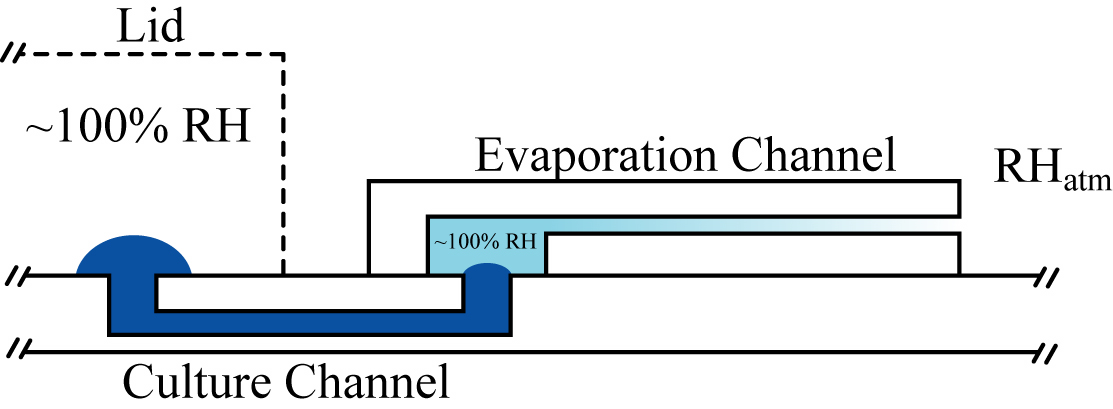
\includegraphics[width=4.5in]{EvaporationChannel.jpg}


\vspace{0.5cm}


b) 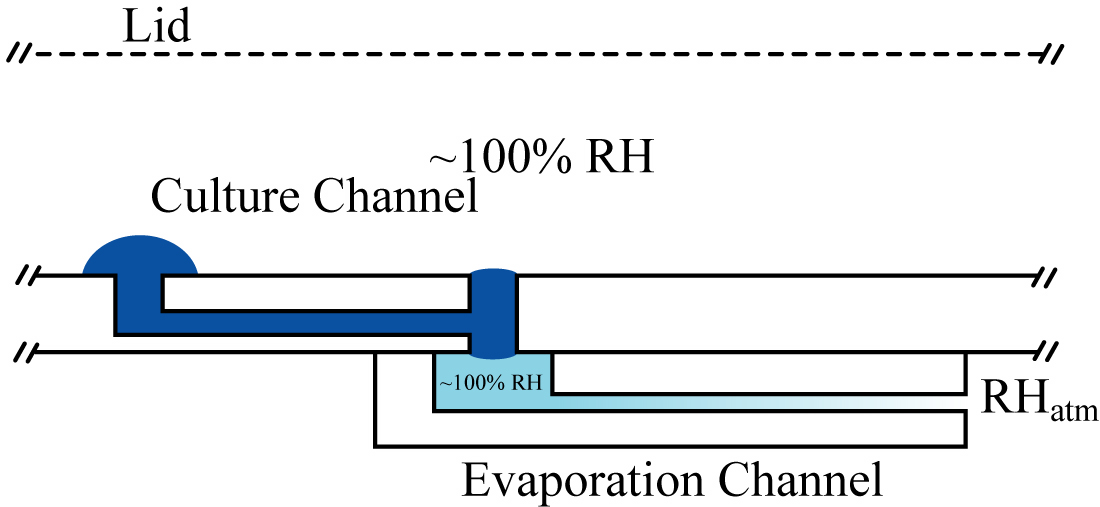
\includegraphics[width=4.5in]{EvaporationChannel2.jpg}
\caption{\textbf{Schematic representation of two different methods for controlling humidity to drive slow flow via evaporation}. The device design minimizes evaporation at non-evaporation ports (\ie , the port on the left) while the evaporation channel is an empty microchannel that resists evaporation at a rate proportional to the ratio of length to cross-sectional area. Varying the length of the evaporation channel linearly varies the evaporation rate and thus the flow through the device. a) Method 1 - Top-Side Evaporation Channel:  Both ports of the device are on the top-side of the substrate. b) Method 2 - Bottom-Side Evaporation Channel:  The evaporation channel is situated on the bottom-side of the substrate by creating a hole through the substrate. Preliminary results suggest the bottom-side design has advantages with respect to sterilization procedures, ease of use, and compatibility with PDMS and a material for making the microchannels.}
%Method 1) Two chamber design with variable sacrificial fluid. The inner chamber attempts to minimize evaporation from the non-evaporation ports while the exterior chamber controls evaporation through an appropriate amount and placement of sacrificial fluid (empirically determined) [CITE JAY/ERWIN].
\label{fig:evaporationDevices}
\end{figure}

The two designs implement the use of an evaporation vent. The evaporation vent is a microchannel that is left unfilled. One end of the channel has a port that encloses the evaporation port of the perfusion device. Vapor that is diffusing away from the evaporation port must diffuse through the evaporation vent. Therefore, the flux of vapor from the evaporation vent can be controlled by designing the cross-sectional area and length of the channel resist evaporation appropriately for the external humidity conditions. The resistance of the evaporation vent to vapor diffusion is proportional to the ratio of its length to its cross-sectional area. Silica beads will be used to control the external humidity at the underside of the device. 

%The major advantage using the evaporation vent is that the humidity external to the device does not need to be controlled such as with the use of a standard cell culture incubator. This makes the device much more portable and robust to external changes in humidity. If the evaporation vent is designed for dry external environments, then the device will better suited for the environments typical of microscopes or culture hoods, also it could eliminate the requirement for a humidified culture incubator. 

As this method is intended for use in cell culture, one obstacle to the implementation of an evaporation driven method for flow is the accumulation of solute near the evaporation port. Over the time-course of evaporation, increased osmolarity or high concentrations of toxic factors, if allowed to reach the culture region of the device, could adversely effect results. A diffusion valve that was developed in previous work with Erwin Berthier and used in previous work by lab members \cite{Frisk:2008pi} will be used to keep accumulation of solute from diffusing into regions used for cell culture. The diffusion valve is a microchannel with cross-sectional area to length ratio such that when a predetermined flow rate exists through the valve, solute, including small molecules such as ions, cannot diffuse significantly upstream. Thus, given two chambers connected by a diffusion valve, the upstream chamber is diffusionally isolated from the downstream chamber. 

Fig \ref{fig:pecletFlow} shows a plot of normalized concentration versus normalized length within the diffusion valve region given flows of various characteristic Peclet numbers. The Peclet number describes the balance between convective and diffusive transport given a fluid velocity, characteristic length, and diffusion coefficient (Pe = $L\,v/D$). The characteristic length that is appropriate for the diffusion valve is the valve length, as we are interested in transport along the length of the channel. Peclet numbers of ~3.0 suggest that, at stead-state, the upstream chamber is at 5\% the concentration of the downstream chamber. Some similar calculations include $\sim$4.6 $\rightarrow$ 1\%, $\sim$10 $\rightarrow$ 0.004\%, and $\sim$15 $\rightarrow$ 0.00003\%. It may seem extreme to look at such high values of the Peclet but many soluble factors can illicit cellular responses over many orders of magnitude of concentration. However, the calculations suggest that the upstream chamber can be effectively isolated from the downstream chambers.

A more detailed treatment of the diffusion valve including governing equations is contained in the Appendix.

\begin{figure}[!ht]
\centering
\includegraphics[width=3.5in]{DiffusionValve.pdf}
\caption{\textbf{Diffusion valve operation}. Plot of normalized concentration ratio (concentration at position $x/L$ divided by concentration at inlet of the downstream chamber) for various values of the Peclet number for the diffusion valve. $x/L=0$ is at the downstream chamber and $x/L=1$ is at the upstream chamber.}
\label{fig:pecletFlow}
\end{figure}

Another important consideration in the design of slow flow methods such as this is the range of appropriate flow rates for any attached culture chambers. The goal of future work is to create slow perfusion flow without significantly affecting the diffusive transport of factors locally within each culture chamber. Just as the diffusion analysis of Fig \ref{fig:pecletFlow} applies to the diffusion valve, it also applies to the culture chambers. Therefore, a desirable situation would be to keep the Peclet number below a value of 1 in the culture chamber, thereby attempting to minimize the gradient of factors that exist in the culture chamber. The diffusion valve is aimed at isolating small molecules while the culture chambers are aimed at evenly distributing large molecules. This disparity is accounted for in the designing of the relative lengths and widths of the culture chambers and diffusion valves. If the Peclet number is too high in the culture chamber, the cross-sectional area of the culture chamber can be increased or the chamber length can be reduced or, if it easier to modify the diffusion valve, the diffusion valve could be reduced in cross-sectional area or lengthened. These changes in dimensions allow the user to design chambers and valves to the particular flow or media exchange rate that is desired for culture chamber. Thus, fluid exchange rates can be adjusted to increase or decrease overall levels of accumulating factor and still maintain relatively even distributions of factor within the chamber.

The design parameters of the evaporation-based device are listed in Tab \ref{tab:evaporation}.

\begin{table}[!ht]
\centering
\begin{tabular}{ll} \toprule
Parameter & Decription \cr \midrule
$D_{d}$ & {\underline D}iffusion coefficient of solute of interest in the {\underline d}iffusion valve \cr
$D_{c}$ & {\underline D}iffusion coefficient of solute of interest in the {\underline c}ulture chamber \cr
$L_{d}$ & {\underline L}ength of the {\underline d}iffusion valve \cr
$L_{c}$ & {\underline L}ength of the {\underline c}ulture chamber \cr
$L_{e}$ & {\underline L}ength of the {\underline e}vaporation vent \cr
$A_{d}$ & Cross-sectional {\underline a}rea of the {\underline d}iffusion valve \cr
$A_{c}$ & Cross-sectional {\underline a}rea of the {\underline c}ulture chamber \cr
$A_{e}$ & Cross-sectional {\underline a}rea of the {\underline e}vaporation vent \cr
$RH$ & The {\underline r}elative {\underline h}umidity external to the device \cr \bottomrule
\end{tabular}
\caption{\textbf{Table of design parameters for evaporation mediated slow flow device}.}
\label{tab:evaporation}
\end{table}

\subsubsection{Surfactant Mediated Flow}\label{sec:deviceDesignSurf}
Just as surface tension plays the dominant role in producing flow via traditional \pp , surface tension can be modified to produce flow without any addition of fluid. In this device, surfactant is delivered to the output port of the device to cause a change in surface tension resulting in a pressure change that then causes flow in the perfusion device. Our chosen method of surfactant delivery is diffusion through a microchannel. Therefore, the time-scales of the flow are limited by diffusion and can be many hours, as dictated by the geometry of the delivery channel and reservoirs. The total volume pumped via this method is limited by the volumes of the input and output drop of the channel that is being influenced. The fluid velocity within the channel will be a result of the diffusion kinetics, the droplet sizes, and finally the channel geometry. One advantage of this design is that the volumes pumped are small and the fluid flow rate is limited by diffusion, therefore, very slow flow rates can be achieved in a controlled manner. A schematic of the device is shown in Fig \ref{fig:surfactantDevices}.

\begin{figure}[!ht]
\centering
\includegraphics[width=5in]{SurfactantFlowDiagram.pdf}
\caption{\textbf{Slow flow via surfactant diffusion}. Schematic representation of slow perfusion device mediated by controlled delivery of surfactants. Diffusion of surfactant reduces surface tension at the affected output drop. The reduced surface tension causes fluid to flow towards the affected output drop from other input ports in amounts related to the input port radii. Inputs with larger radii will be larger sources of flow. The diffusion valve can be designed to isolate the surfactant from upstream culture areas.}
\label{fig:surfactantDevices}
\end{figure}

The slow flow device shown in Fig \ref{fig:surfactantDevices}, is designed to validate the surfactant-based slow flow method and is not intended for culture. One or multiple culture chambers and their associated ports can be included upstream of the diffusion valve, which is in place to isolate surfactant from the culture components. As mentioned earlier, the diffusion valve is very effective at minimizing diffusion upstream for flows with a Peclet number significantly greater than 1. The output port is connected to a surfactant delivery channel and port. When very small volume of containing a high concentration of surfactant is placed at the surfactant delivery port, negligible flow will occur from \pp\ as the surfactant delivery port has a very small radius. The surfactant will then diffuse through the surfactant delivery channel to affect the output drop. Surfactant diffusing into the output drop will cause a reduction in surface tension and pressure. The loss of pressure causes flow towards the output drop, thereby producing flow for the diffusion valve to isolate surfactant from any upstream culture components.

%Specific dimensions were chosen via simulation of the device in Matlab using 1D simplified models of diffusion in the microchannel. The model assumes even mixing in the output port and a linear relationship between surfactant concentration and surface tension. The model was simulated for a range of surface tensions that would produce a $\sim$70\% reduction in surface tension at the output port (see Appendix). 

Initial simulations suggest that the diffusion process can be made to last hours or days with appropriate geometries. Over those time-courses, input and output volumes can be chosen to result in flow rates that would result in exchange of culture chamber media from fractions per day up to many times per day suggesting that it would be an appropriate method for slow perfusion microchannel culture.

Design parameters of the device, when used to perfuse fluid through a culture chamber are very similar to the evaporation based device with slight differences as shown in Tab \ref{tab:surfactant}.

\begin{table}[!ht]
\centering
\begin{tabular}{ll} \toprule
Parameter & Decription \cr \midrule
$D_{d}$ & {\underline D}iffusion coefficient of solute of interest in the {\underline d}iffusion valve \cr
$D_{c}$ & {\underline D}iffusion coefficient of solute of interest in the {\underline c}ulture chamber \cr
$D_{s}$ & {\underline D}iffusion coefficient of {\underline s}urfactant \cr
$L_{d}$ & {\underline L}ength of the {\underline d}iffusion valve \cr
$L_{c}$ & {\underline L}ength of the {\underline c}ulture chamber \cr
$L_{s}$ & {\underline L}ength of the {\underline s}urfactant delivery channel \cr
$A_{d}$ & Cross-sectional {\underline a}rea of the {\underline d}iffusion valve \cr
$A_{c}$ & Cross-sectional {\underline a}rea of the {\underline c}ulture chamber \cr
$A_{s}$ & Cross-sectional {\underline a}rea of the {\underline s}urfactant delivery channel \cr
$S$ & The type of {\underline s}urfactant delivered \cr \bottomrule
\end{tabular}
\caption{\textbf{Table of design parameters for surfactant mediated slow flow device}.}
\label{tab:surfactant}
\end{table}

One important unknown aspect of the design suggested by the parameter $S$ in Tab \ref{tab:surfactant} is the identity of the surfactant and the effectiveness of the surfactant to reduce surface tension in the media. A preliminary experiment will be performed using a goniometer to determine the surface tension profile of different concentrations of surfactant and media. The profile will influence the flow rate progression over time and will be important to evaluating the ability of this method to produce consistent flow over long intervals. One surfactant of interest is bovine serum albumin (BSA).

\subsection{Methods}

Methods common to many pieces of the work proposed here are described in the Appendix such as device manufacture and modeling of diffusion, signaling, and response.

\subsubsection{Device Characterization}
The device designs will be characterized by measuring total flow over time and observing the quasi-steady-state convection-diffusion of dye or fluorescently labeled molecules at different times. In the case of the evaporation-based slow flow device, flow will be measured as the total volume loss over time compared to a `no evaporation' control, whereas in the case of the surfactant mediated flow device, droplet profile will be measured at the input port to infer volume at various time-points and will also be compared to a `no evaporation' control.

\subsection{Preliminary Results} \label{sec:prelimCCResults}

Some preliminary testing has already been accomplished with respect to slow-perfusion via evaporation. However, the results were obtained in the context of work towards a `one-way co-culture' device and thus diagrams show devices that have two chambers instead of one as suggested in section \ref{sec:deviceDesignEvap}. Fig \ref{fig:oneWayDye}a shows images of a slow-perfusion device with two culture chambers. Each image shows a different scenario. The bright-field image is intended to show the shape of the device. The balloons labeled with the word `add' indicate that fluorescent dye was added to the chamber prior to flow. The images with the square chambers are simulation results false colored like the dye. In each case, the dye in the experiment and simulation are confined to be at or below the chamber to which it was added over the course of 24 hours. Thus, evaporation was successfully implemented to direct a slow flow that transports fluid at similar rates to diffusion in the culture chambers and the diffusion valves were effective barriers to diffusion upstream. The fluid velocity simulation diagram of Fig \ref{fig:oneWayDye} indicates the relative flow rates that exist in the diffusion valves versus the chambers.

\begin{figure}[!ht]
\begin{center}
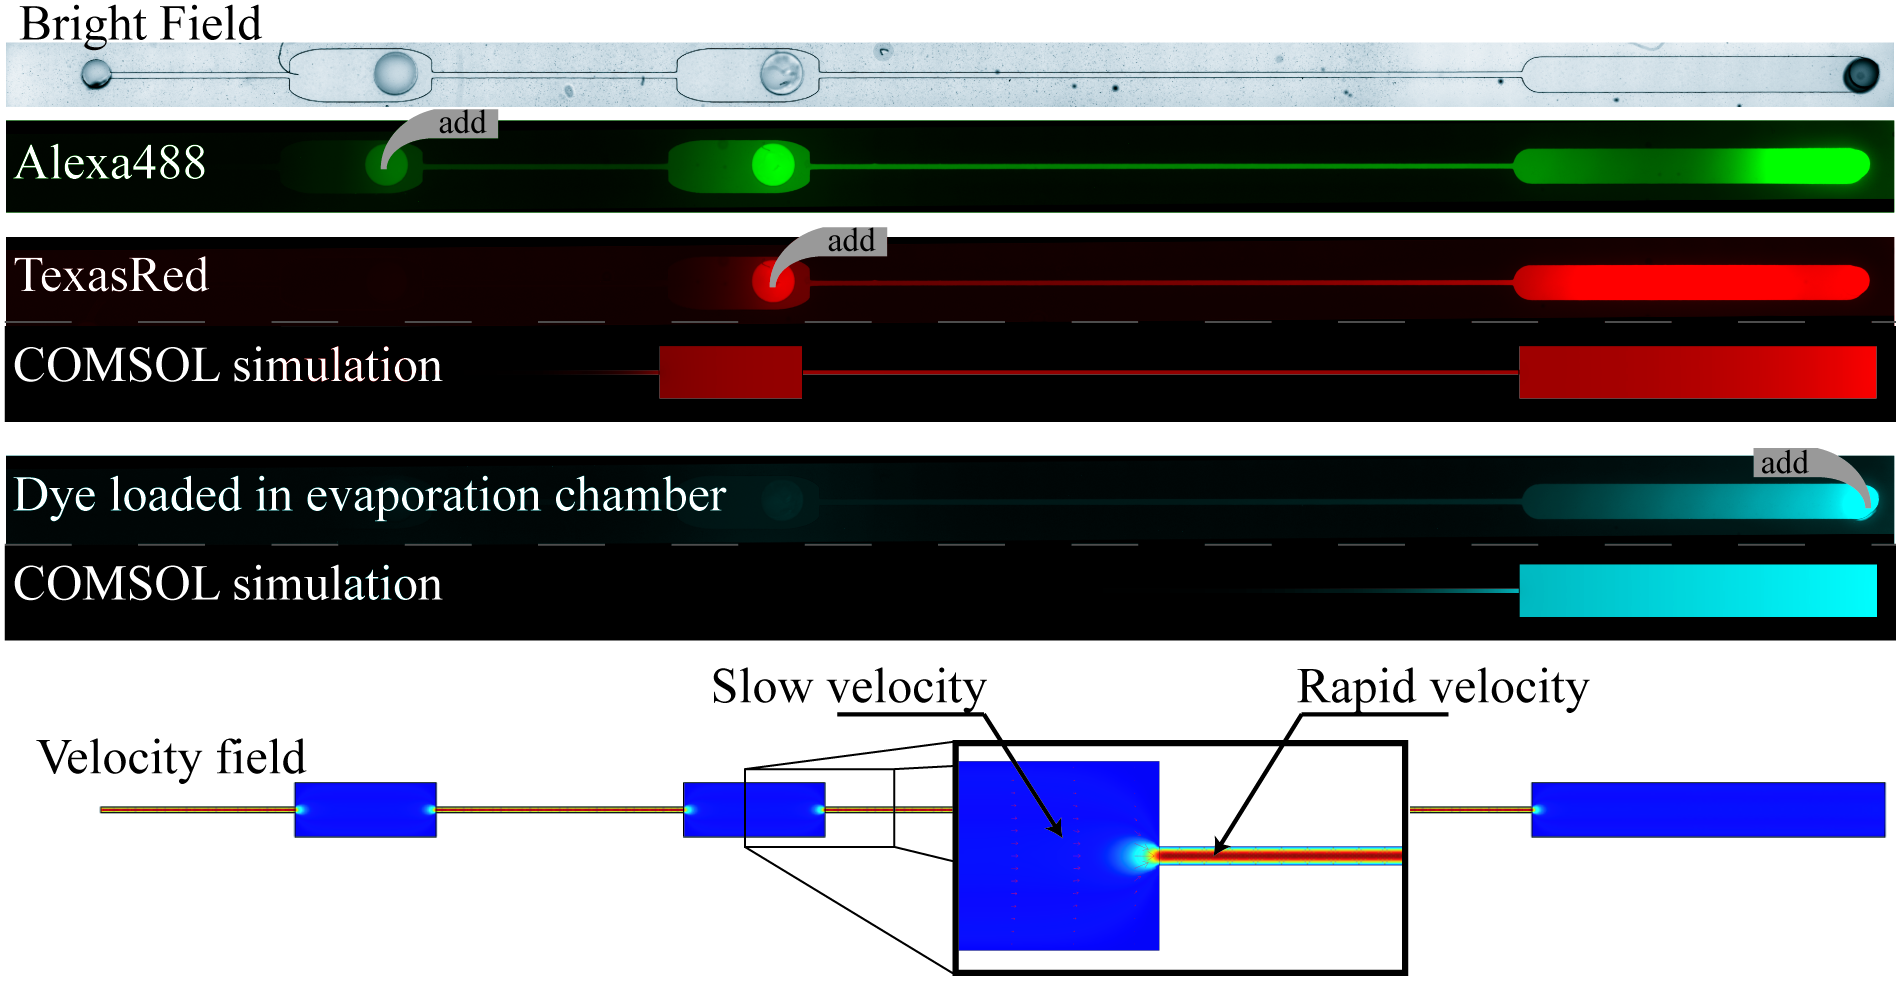
\includegraphics[width=6.5in]{OneWay_Illustration_figure.png}
\caption{\textbf{Preliminary validation of real-time conditioned media assay device operation}. Microscope images demonstrating the function of the diffusion valve. Different dyes (Alexa488 and TexasRed bound to Dextran 10kD) were loaded in the chambers destined for cell culture and imaged after 24 hours. The profiles show the presence of dyes downstream of diffusion valves but not upstream. COMSOL simulations were performed by supposing constant production of dye in the chamber after 20 hours. The velocity fields obtained are displayed.}
\label{fig:oneWayDye}
\end{center}
\end{figure}

\subsection{Expected Challenges}
Preliminary results suggest that there will be some challenges with respect to the technical implementation. One of the evaporation designs requires cutting through the polystyrene substrate, which can be a challenge. However, we have just purchased a CO$_{2}$ laser cutting system which has the capability to cut holes through polystyrene with sufficient accuracy. Processing parameters for optimal hole manufacture are still undetermined but is the focus of a hired undergraduate over the semester.

Further, the evaporation device that requires laser cutting will also need a method to create a dry environment on the bottom side of the device. Preliminary tests have shown that we can either use a sealed lid and a dry incubator or a non-sealed lid and a sealed chamber under the channel in which humidity is depleted using silica beads. The latter appears to have the most advantages as it allows for a more free gas exchange with the gas controlled incubator. However, the capacity of the silica beads to maintain a dry environment has not been thoroughly investigated but first indications are that they are quite sufficient.

\paragraph{Side note for future work:}Just as silica beads can be used to create an atmosphere depleted of water vapor at the underside of the evaporation device, other materials exist that can deplete or supply other gaseous molecules such as oxygen. In this way, different concentrations of gaseous molecules could be maintained at each end of a microchannel to create gradients. The work proposed here represents a first step towards such gradient devices that could be a way to readily examine the effects of microenvironmental parameters such as oxygen tension.

\section{Cross Flow in the Diffusion Region}
The following fluidic device can be analyzed using an electrical analogy (see Fig \ref{App:PerfusionCulture:fig:device}). The electric circuit analogy can be split into an analogous circuit in which there are two voltage sources. Now the problem can be solved using superposition. When using superposition, one voltage source is disconnected and the circuit is solved. The same is done using the other as the sole voltage source. This solutions are then added to obtain total voltages and currents which should match the results of the original circuit. 

\begin{figure}[!ht]
\centering
a) \includegraphics[height=2in]{Device.pdf}     b) \includegraphics[height=2in]{Original.pdf}
\caption{\textbf{Perfusion co-culture}. Perfusion co-culture device in which flow ratios will be estimated and its electric circuit analog.}
\label{App:PerfusionCulture:fig:device}
\end{figure}

Fig \ref{fig:circuit} shows two circuits, that when solved and their solutions added together, give the solution to the original circuit shown in Fig \ref{App:PerfusionCulture:fig:device}.

\begin{figure}[!ht]
\centering
\includegraphics[height=2in]{Analog.pdf}
\caption{\textbf{Perfusion co-culture circuit analog}. Diagrams of circuits that when added together, are equivalent to the original circuit of Fig \ref{App:PerfusionCulture:fig:device}. The circuits shown here are easier to solve and are used in the math that follows to find the ratios of currents or fluid flows through the device as compared to the total flow through the device.}
\label{fig:circuit}
\end{figure}

The left-hand and right-hand circuit have the following equivalent resistances.

\begin{equation}
R_{LH} = R_{1} + \frac{1}{\frac{1}{R_{4}} + \frac{1}{C_{LH}}}\textrm{, where } C_{LH} = R_{3} + \frac{1}{\frac{1}{R_{5}} + \frac{1}{R_{2}}}
\end{equation}
\begin{equation}
R_{RH} = R_{2} + \frac{1}{\frac{1}{R_{5}} + \frac{1}{C_{RH}}} \textrm{, where } C_{RH} = R_{3} + \frac{1}{\frac{1}{R_{4}} + \frac{1}{R_{1}}}
\end{equation}

Therefore the ratio $I_{1}/I_{2}$ is equal to the ratio $R_{RH}/R_{LH}$. Now if we solve for $I_{3}$ in each circuit, we can use the information to indicate the proporation of total current through the circuit that is devoted to pass through $R_{3}$ (\ie , the fluid flow through the diffusion valve).

In the left-hand circuit, 
\begin{equation}
I_{2}^{LH} =\frac{V}{R_{LH}}
\end{equation}
\begin{equation}
I_{3}^{LH} =\frac{I_{1}^{LH}}{1+ \frac{C_{LH}}{R4}}
\label{equ:LHI3}
\end{equation}
\begin{equation}
I_{2}^{LH} =\frac{I_{3}^{LH}}{1+\frac{R_{2}}{R_{5}}}
\end{equation}
and in the right-hand circuit
\begin{equation}
I_{1}^{RH} =\frac{V}{R_{RH}}
\end{equation}
\begin{equation}
I_{3}^{RH} =\frac{I_{1}^{RH}}{1+ \frac{C_{RH}}{R5}}
\label{equ:LHI3b}
\end{equation}
\begin{equation}
I_{1}^{RH} =\frac{I_{3}^{RH}}{1+\frac{R_{1}}{R_{4}}}
\end{equation}
and by superposition,
\begin{equation}
I_{3} = I_{3}^{LH} - I_{3}^{RH}
\label{equ:I3}
\end{equation}
\begin{equation}
I_{1} = I_{1}^{LH} - I_{1}^{RH}
\label{equ:I1}
\end{equation}
\begin{equation}
I_{2} = I_{2}^{RH} - I_{2}^{LH}
\label{equ:I2}
\end{equation}

The minus sign is to indicate that the $I_{1}$, $I_{2}$, and $I_{3}$ currents are in opposite directions in the RH and LH circuits. This then allows us to write the proportion of total current that flows through the diffusion region as the following.

\begin{equation}
\textrm{Cross Flow Ratio} = \frac{I_{3, tot}}{I_{1} + I_{2}}
\end{equation}

Using the above equations Fig \ref{fig:crossFlow} was created to observe the influence of unbalanced resistance on the rate of cross flow through the bridge relative to the total flow through the device. This is done by varying only the resistance of $R_{5}$.

\begin{figure}[!ht]
\centering
\includegraphics[width=3.5in]{CrossFlowPlot.pdf}
\caption{\textbf{Cross-flow during perfusion co-culture}. Calculations of relative cross flow rate using electrical analog equations for different output resistance ratios.}
\label{fig:crossFlow}
\end{figure}

\section{Peclet Ratio}

Diffusive flux in a rectangular duct with 1D diffusion is proportional to the following expression, $J \propto D\,A/L$ where $D$ is the diffusion coefficient describing the solvent and solute, $A$ is the cross-sectional area of the duct, and $L$ is the length of the duct. Therefore, to maximize the flux through the diffusion region we would like to maximize $A$ and minimize $L$.

In order to maximize diffusive flux in the parallel perfusion co-culture device the diffusion region length, $h_{d}$, will likely be the same height as the culture region, $h_{c}$, and the length roughly 1/10$^{th}$ the culture chamber length (\ie , $h_{d}/h_{c} \approx 1$, and $L_{d}/L_{c} \approx 0.1$). A significant width for the diffusion region might also be roughly the width of the culture chambers (\ie , $w_{d}/w_{c} \approx 1$).

The Peclet number of a flow is given by $Pe = L\,v/D$ which can also be written in terms of the flow rate for a duct as $Pe = L\, Q \, w \, h/D$. Further, if we estimate the flow rate in each culture chamber as being half of the total flow for a reasonably balanced system, we can write an expression for the ratio of Peclet numbers for the culture chambers versus the diffusion region between the chambers ($Pe_{c}/Pe_{d}$, culture chamber over diffusion region).

\begin{equation}
Pe_{c}/Pe_{d} = \frac{L_{c}Q_{c}w_{c}h_{c}}{L_{d}Q_{d}w_{d}h_{d}}
\end{equation}

Using conclusions from the previous section and assuming the flow in each culture chamber is about half of the total flow through the device, we can estimate the flow rate ratios, $Q_{c}/Q_{d} \approx 0.04$. We have already suggested that $h_{c}/h_{d} \approx 1$, $w_{d}/w_{c} \approx 1$, and $L_{c}/L_{d} \approx 0.1$. Therefore, it is expected that the ratio of the diffusion region Peclet number and culture chamber peclet number will be roughly $0.04 \times 1 \times 1 \times 0.1 \approx 0.004$. Since the aim of the coculture device is to keep the Peclet number in the culture chamber close to 1, the Peclet number in the diffusion region will be $\ll 1$ ensuring relatively unbiased communication between the two chambers.


%Now if we assume the following,
%\begin{equation}
%R1/R2 = \alpha
%\end{equation}
%\begin{equation}
%R4/R5 = \beta
%\end{equation}
%then each of the above equations can be collapsed to the following.

%\begin{equation}
%R_{LH} = \alpha R_{2} + \frac{1}{\frac{1}{\beta R_{5}} + \frac{1}{C_{LH}}}\textrm{, where } C_{LH} = R_{3} + \frac{1}{\frac{1}{R_{5}} + \frac{1}{R_{2}}}
%\end{equation}
%\begin{equation}
%R_{RH} = R_{2} + \frac{1}{\frac{1}{R_{5}} + \frac{1}{C_{RH}}} \textrm{, where } C_{RH} = R_{3} + \frac{1}{\frac{1}{\beta R_{5}} + \frac{1}{\alpha R_{2}}}
%\end{equation}



%		Clh = (R3 + (1/((1/R5) + (1/R2))));
%		System.out.println("Clh: " + Clh);
%		Crh = (R3 + (1/((1/R4) + (1/R1))));
%		System.out.println("Crh: " + Crh);
%		
%		Rlh = R1 + 1/((1/R4) + (1/Clh));
%		System.out.println("Rlh: " + Rlh);
%		Rrh = R2 + 1/((1/R5) + (1/Crh));
%		System.out.println("Rrh: " + Rrh);
%		
%		I1lh = 1/Rlh;
%		System.out.println("I1lh: " + I1lh);
%		I3lh = I1lh/(1+(Clh/R4));
%		System.out.println("I3lh: " + I3lh);
%		I2lh = I3lh/(1+(R2/R5));
%		System.out.println("I2lh: " + I2lh);
%		
%		I2rh = 1/Rrh;
%		System.out.println("I2rh: " + I2rh);
%		I3rh = I2rh/(1+(Crh/R5));
%		System.out.println("I3rh: " + I3rh);
%		I1rh = I3rh/(1+(R1/R4));
%		System.out.println("I1rh: " + I1rh);










% \bibliographystyle{abbrvnat}
% \begin{singlespacing}
% \bibliography{./Bibliography/bib}
\bibliography{mendeley.bib}
% \end{singlespacing}

\printbibliography

\end{document}






















































































